
\documentclass[12pt,letterpaper]{report}
% \usepackage{natbib}
\usepackage[style=nature, citestyle=authoryear, refsegment=chapter]{biblatex}
\usepackage{geometry}
%\usepackage{fancyheadings} fancyheadings is obsolete: replaced by fancyhdr. JL
\usepackage{fancyhdr}
\usepackage{afterpage}
\usepackage{graphicx}
\usepackage{amsmath,amssymb,amsbsy}
\usepackage{dcolumn,array}
\usepackage{tocloft}
\usepackage{asudis}
%adam's packages
% \usepackage{hyperref}
\usepackage{url}
\usepackage{graphicx}
\usepackage{tikz}
\usepackage{wrapfig}
\usepackage{booktabs}
\usepackage{tabularx}
\usepackage{multirow}
\usepackage{minted}
\usepackage{textcase}
% \usepackage{caption}


% \DeclareCaptionLabelFormat{cont}{#1~#2\alph{ContinuedFloat}}
% \captionsetup[ContinuedFloat]{labelformat=cont}


\addglobalbib{ch1/ch1.bib}
\addglobalbib{ch2/ch2.bib}
\addglobalbib{ch3/ch3.bib}
\addglobalbib{ch4/ch4.bib}	
\addglobalbib{ch5/ch5.bib}
\addglobalbib{ch6/ch6.bib}
\setcounter{biburlnumpenalty}{9000}
\setcounter{biburlucpenalty}{9100}
\appto{\bibsetup}{\sloppy}

\renewcommand{\tabularxcolumn}[1]{m{#1}}
\newcommand{\titlecaption}[2]{\caption[#1]{\textbf{#1 \textbar\,} #2}}
\newcommand{\protectedref}[1]{\ref{#1}}
\newcommand{\phylogenomicref}{\ref{ch:phylogenomic}}
\newcommand{\kbbqref}{\ref{ch:kbbq}}
\newcommand{\structuredref}{\ref{ch:structured}}
\newcommand{\evaluatingref}{\ref{ch:evaluating}}
\newcommand{\includetwo}[2]{\begin{minipage}{.475\textwidth}%
\includegraphics[width = \textwidth]{#1}%
\end{minipage}\hfill\begin{minipage}{.475\textwidth}%
\includegraphics[width = \textwidth]{#2}%
\end{minipage}}



\begin{document}
%-----------------------front matter
\pagenumbering{roman}
\title{Methods for Detecting Mutations in Non-model Organisms}
\author{Adam James Orr}
\degreeName{Doctor of Philosophy}
\defensemonth{November}
\gradmonth{December}
\gradyear{2020}
\chair{Reed Cartwright, Chair \\ Melissa Wilson\\ Kenro Kusumi\\ Jay Taylor\\ Susanne Pfeifer}		
\maketitle
\doublespace
\begin{abstract}
Next-generation sequencing is a powerful tool for detecting genetic variation. However, it is also error-prone, with error rates that are much larger than mutation rates. This can make mutation detection difficult; and while increasing sequencing depth can often help, sequence-specific errors and other non-random biases cannot be detected by increased depth. The problem of accurate genotyping is exacerbated when there is not a reference genome or other auxiliary information available.

I explore several methods for sensitively detecting mutations in non-model organisms using an example \textit{Eucalyptus melliodora} individual. I use the structure of the tree to find bounds on its somatic mutation rate and evaluate several algorithms for variant calling. I find that conventional methods are suitable if the genome of a close relative can be adapted to the study organism. However, with structured data, a likelihood framework that is aware of this structure is more accurate. I use the techniques developed here to evaluate a reference-free variant calling algorithm.

I also use this data to evaluate a k-mer based base quality score recalibrator (KBBQ), a tool I developed to recalibrate base quality scores attached to sequencing data. Base quality scores can help detect errors in sequencing reads, but are often inaccurate. The most popular method for correcting this issue requires a known set of variant sites, which is unavailable in most cases. I simulate data and show that errors in this set of variant sites can cause calibration errors. I then show that KBBQ accurately recalibrates base quality scores while requiring no reference or other information and performs as well as other methods.

Finally, I use the \textit{Eucalyptus} data to investigate the impact of quality score calibration on the quality of output variant calls and show that improved base quality score calibration increases the sensitivity and reduces the false positive rate of a variant calling algorithm.

\end{abstract}

\dedicationpage{For my family. They taught me to be curious, tenacious, and persistent; to believe in myself, do my best, and never give up.}

\begin{acknowledgements}
Thanks to my advisor, whose input helped substantially improve this work and for giving me the space and support I needed to work and grow.
Thanks to my committee, whose input substantially improved this dissertation and the work described herein.
Thanks to the members of my lab past and present, who created a cordial, pleasant, and intellectually stimulating environment to work in and provided helpful feedback.
Thanks to the Arizona State University School of Life Sciences and College of Liberal Arts and Sciences for the Spring 2020 Completion Fellowship, which greatly improved this dissertation.
Thanks to the National Science Foundation, National Institutes of Health, and U.S.-Israel Binational Science Foundation  which funded parts of this work.

\end{acknowledgements}
\tableofcontents
% This puts the word "Page" right justified above everything else.
\addtocontents{toc}{~\hfill Page\par}
% Asking LaTeX for a new page here guarantees that the LOF is on a separate page
% after the TOC ends.
\newpage
% Making the LOT and LOF "parts" rather than chapters gets them indented at
% level -1 according to the chart: top of page 4 of the document at
% ftp://tug.ctan.org/pub/tex-archive/macros/latex/contrib/tocloft/tocloft.pdf

% This gets the headers for the LOT right on the first page.  Subsequent pages
% are handled by the fancyhdr code in the asudis.sty file.
\addcontentsline{toc}{part}{LIST OF TABLES}
\listoftables
\addtocontents{lot}{Table~\hfill Page \par}
\newpage
\addcontentsline{toc}{part}{LIST OF FIGURES}
\addtocontents{toc}{CHAPTER \par}
\listoffigures
\addtocontents{lof}{Figure~\hfill Page \par}
\newpage

% This gets the headers for the LOF right on the first page.  Subsequent pages
% are handled by the fancyhdr code in the asudis.sty file.

\graphicspath{{ch2/figures/}{ch3/figures/}{ch4/figures/}{ch5/figures/}{defense/figures/}}

%-----------------------body
\doublespace
\pagenumbering{arabic}
\chapter{Introduction}

%A brief introduction that introduces topics like DNA sequencing and variant calling. Also introduces the \textit{E. melliodora} dataset used in the 2nd, 3rd, and 5th chapters.

%TODO: MANY CITES ! These things are all gonna need citations.
%TODO: maybe more background info?

Next-generation sequencing is a powerful technology with numerous applications. It has enabled data collection and hypothesis testing at an unprecedented scale, with an enormous amount of sequencing data generated daily \parencite{kodama_sequence_2012}. The high-throughput nature of modern sequencing technologies makes it cheap and efficient to genotype one or more samples. Additionally, next-generation sequencing serves as the basis of a variety of methods for interrogating a wide array of molecular functions and epigenetic states including RNA-seq \parencite{nagalakshmi_transcriptional_2008}, ChIP-seq \parencite{johnson_genome-wide_2007}, DNase-seq \parencite{boyle_high-resolution_2008}, MNAse-seq \parencite{schones_dynamic_2008}, ATAC-seq \parencite{buenrostro_atac-seq_2015}, bisfulfite sequencing \parencite{frommer_genomic_1992}, and many more. As a testament to how powerful and useful the technology is for understanding the natural world, it has achieved such widespread use despite being highly error-prone \parencite{nakamura_sequence-specific_2011, meacham_identification_2011, fox_accuracy_2014}. DNA sequencing technology continues to improve; increasing read length and reduced substitution, insertion, and deletion errors are seemingly inevitable as new methods develop and the technology is refined \parencite{branton_potential_2008, eid_real-time_2009, fox_accuracy_2014}. Yet even the most sophisticated and accurate sequencing platforms will require analysis with sound statistical methods to turn raw data into interesting and useful insights about the natural world.

In this dissertation, I explore and develop methods for gaining insight from noisy next-generation sequencing data in challenging contexts. In particular, I focus on genotyping and detecting mutations in non-model organisms. While there has been an explosion in the amount of sequencing data generated since the advent of the technology, most species on the planet have still not been sequenced; even fewer have complete and accurate reference genomes \parencite{lewin_earth_2018}. Yet, funding available specifically for the generation and refinement of new reference genomes is difficult to acquire \parencite{richards_its_2015}. Model organisms are immensely useful for generating knowledge and are vital to gaining understanding of the world; however, it is clear that model organisms do not hold the answers to every interesting question. As such, it is important and necessary to develop methods for data analysis that work well even with limited \textit{a priori} knowledge.

In the second chapter, I present collaborative work on sensitively detecting somatic mutations in the non-model eucalypt, \textit{Eucalyptus melliodora}. This work was previously published in \textit{Proceedings of the Royal Society B} and documents my and my coauthors' efforts to estimate the somatic mutation rate of an individual eucalypt. As a control, I used a conventional variant calling algorithm paired with custom filters to investigate whether the physical tree structure of the organism also gives it a tree-like genetic structure, as one may predict based on how trees grow and mature. I also investigate the limits of this approach and find bounds on the estimates of several population genetic parameters we are able to estimate from the data.

The sequencing data and calls made in the second chapter are used throughout this dissertation as a basis of comparison for many of the techniques I use. The third chapter details my investigation of base quality score recalibration, a technique used to fix inaccurate quality measurements attached to sequencing data. I introduce an efficient software program \texttt{kbbq} to perform base quality score recalibration on whole genome sequencing reads without a reference genome or other \textit{a priori} knowledge and show it performs just as well as the most common method for base quality score recalibration.

Errors are common relative to mutations in sequencing data, \parencite{fox_accuracy_2014, wu_estimating_2017} and since correlated errors are by definition non-independent, such errors cannot be detected by increased sequencing depth alone \parencite{meacham_identification_2011, taub_overcoming_2010}. Correcting quality score calibration issues in sequencing reads could in principle improve the ability of a variant caller to distinguish between true variation and noise in a way that increased depth cannot. While there is some evidence that it does help increase sensitivity \parencite{ni_improvement_2016}, it is an open question whether the benefits of base quality score recalibration outweigh the time, computational cost, and risk of introducing additional error. While the process has long been a part of the GATK Best Practices pipeline, it has recently fallen out of favor \parencite{van_der_auwera_geraldine_2020_b}. In the fourth chapter, I investigate the effect of base quality score recalibration on variant caller sensitivity and specificity.

%TODO: make this not suck
All together, this work explores many avenues for detecting variants in non-model organisms. 
There are many ways to do so, and many more that aren't discussed here.
Each has strengths and weaknesses, but understanding what these are is critical to success.
While choosing the correct method can be a challenging and daunting task, with careful preparation and rigorous examination of the available methods, any researcher can achieve satisfactory results.

\printbibliography[segment=\therefsegment]{}

\chapter{A phylogenomic approach reveals a low somatic mutation rate in a long-lived plant}
\label{ch:phylogenomic}

\parindent0pt by Adam J. Orr\textsuperscript{\dagger}, Amanda Padovan\textsuperscript{\dagger}, David Kainer\textsuperscript{\dagger}, Carsten Külheim, Lindell Bromham, Carlos Bustos-Segura, William Foley, Tonya Haff, Ji-Fan Hsieh, Alejandro Morales-Suarez, Reed A. Cartwright, and Robert Lanfear
\\
\hspace*{\fill}\textit{\dagger Equal contribution.}

\vspace{\baselineskip}

\textit{This chapter was originally published as an article in} Proceedings of the Royal Society B \textit{with }\texttt{doi:10.1098/rspb.2019.2364}\textit{. It is available under the CC-BY-4.0 license }\texttt{https://creativecommons.org/licenses/by/4.0/}\textit{ and is included with permission of the authors (see Appendix \ref{ch:permission}).}

\section{Abstract}
Somatic mutations can have important effects on the life history, ecology, and evolution of plants, but the rate at which they accumulate is poorly understood and difficult to measure directly. Here, we develop a method to measure somatic mutations in individual plants and use it to estimate the somatic mutation rate in a large, long-lived, phenotypically mosaic \textit{Eucalyptus melliodora} tree. Despite being 100 times larger than \textit{Arabidopsis}, this tree has a per-generation mutation rate only ten times greater, which suggests that this species may have evolved mechanisms to reduce the mutation rate per unit of growth. This adds to a growing body of evidence that illuminates the correlated evolutionary shifts in mutation rate and life history in plants.

\section{Background}

Trees grow from multiple meristems which contain stem cells that divide to produce the somatic and reproductive tissues. A mutation occurring in a meristematic cell will be passed on to all resulting tissues, potentially causing an entire branch including leaves, stems, flowers, seeds, and pollen to have a genotype different from the rest of the plant \parencite{plomion_oak_2018, schmid-siegert_low_2017}. These different genotypes may lead to phenotypic changes, potentially with important consequences for plant ecology and evolution \parencite{whitham_evolution_1981, buss_evolution_1983, walbot_life_1985, sutherland_somatic_1986, klekowski_ageing_1989, ally_aging_2010}. For example, somatic mutations could explain how long-lived plants adapt to changing ecological conditions \parencite{gill_genetic_1995}, and are thought to influence long-term variation in the rates of evolution and speciation among plant lineages \parencite{lanfear_taller_2013}. Somatic mutations can degrade genetic stocks used in agriculture and forestry \parencite{khoury_trends_2010, schoen_deleterious_1998}, confer herbicide resistance to weed species, \parencite{michel_somatic_2004} and have been linked to declining plant fitness in polluted areas \parencite{klekowski_petroleum_1994}. However, despite the importance of somatic mutations and recent progress in understanding them \parencite{plomion_oak_2018, schmid-siegert_low_2017, hanlon_somatic_2019, wang_architecture_2019, schultz_mutation_2009, bobiwash_somatic_2013}, there remain significant analytical challenged in inferring somatic mutation rates from sequencing data in plants.

We present a solution to the challenges of measuring the somatic mutation rate that leverages the phylogeny-like structure of the plant itself to estimate the genome-wide somatic mutation rate of the individual. Our strategy has three key features. First, we sequence the full genome of three biological replicates of eight branch tips. Using three biological replicates per branch tip significantly reduces the false-positive rate, because many types of error (e.g. sequencing error or mutations induced during DNA extraction or library preparation) are very unlikely to appear at the same position in all three replicates, making it easy to distinguish these errors from biological signal. Second, our strategy includes an inbuilt positive control, because we can ask whether the phylogenetic tree we reconstruct from the set of putative somatic mutations across the eight branch tips reflects the known physical structure of the tree (i.e. whether phylogeny correctly reconstructs ontogeny, as is expected for plant development in most cases, but see below). Third, the approach allows us to estimate the false-negative rate and the false-discovery rate of our inferences directly from the replicate samples (see below).

We applied this approach to a long-lived yellow box (\textit{Eucalyptus melliodora}) tree, notable for its phenotypic mosaicism: a single large branch in this individual is resistant to defoliation by Christmas beetles (\textit{Anoplognathus} spp Coleoptera: Scarabaeidae) due to stable differences in leaf chemistry and gene expression \parencite{padovan_differences_2013, edwards_mosaic_1990}. We find that the rate of somatic mutation per generation is relatively high, but the rate per metre of growth is surprisingly low in comparison to other species. We suggest potential proximate and ultimate reasons for the wide variation in somatic mutation rates across plants.


\section{Materials and methods}

\subsection{Field sampling}

We used a known mosaic \textit{E. melliodora} (yellow box). This tree is found near Yeoval, NSW, Australia (-32.75°, 148.65°). We collected the ends of eight branches in the canopy (figure \ref{fig:emel_1}). Branches were collected using an elevated platform mounted on a truck and were placed into labelled and sealed polyethylene bags which were immediately buried in dry ice in the field. Within the 24 h of collection, the samples were transferred to -80°C until DNA extraction. Simultaneously, we used a thin rope to trace each branch from the tip to the main stem. These rope lengths were measured to determine the lengths of the physical branches of the tree. 

\begin{figure}
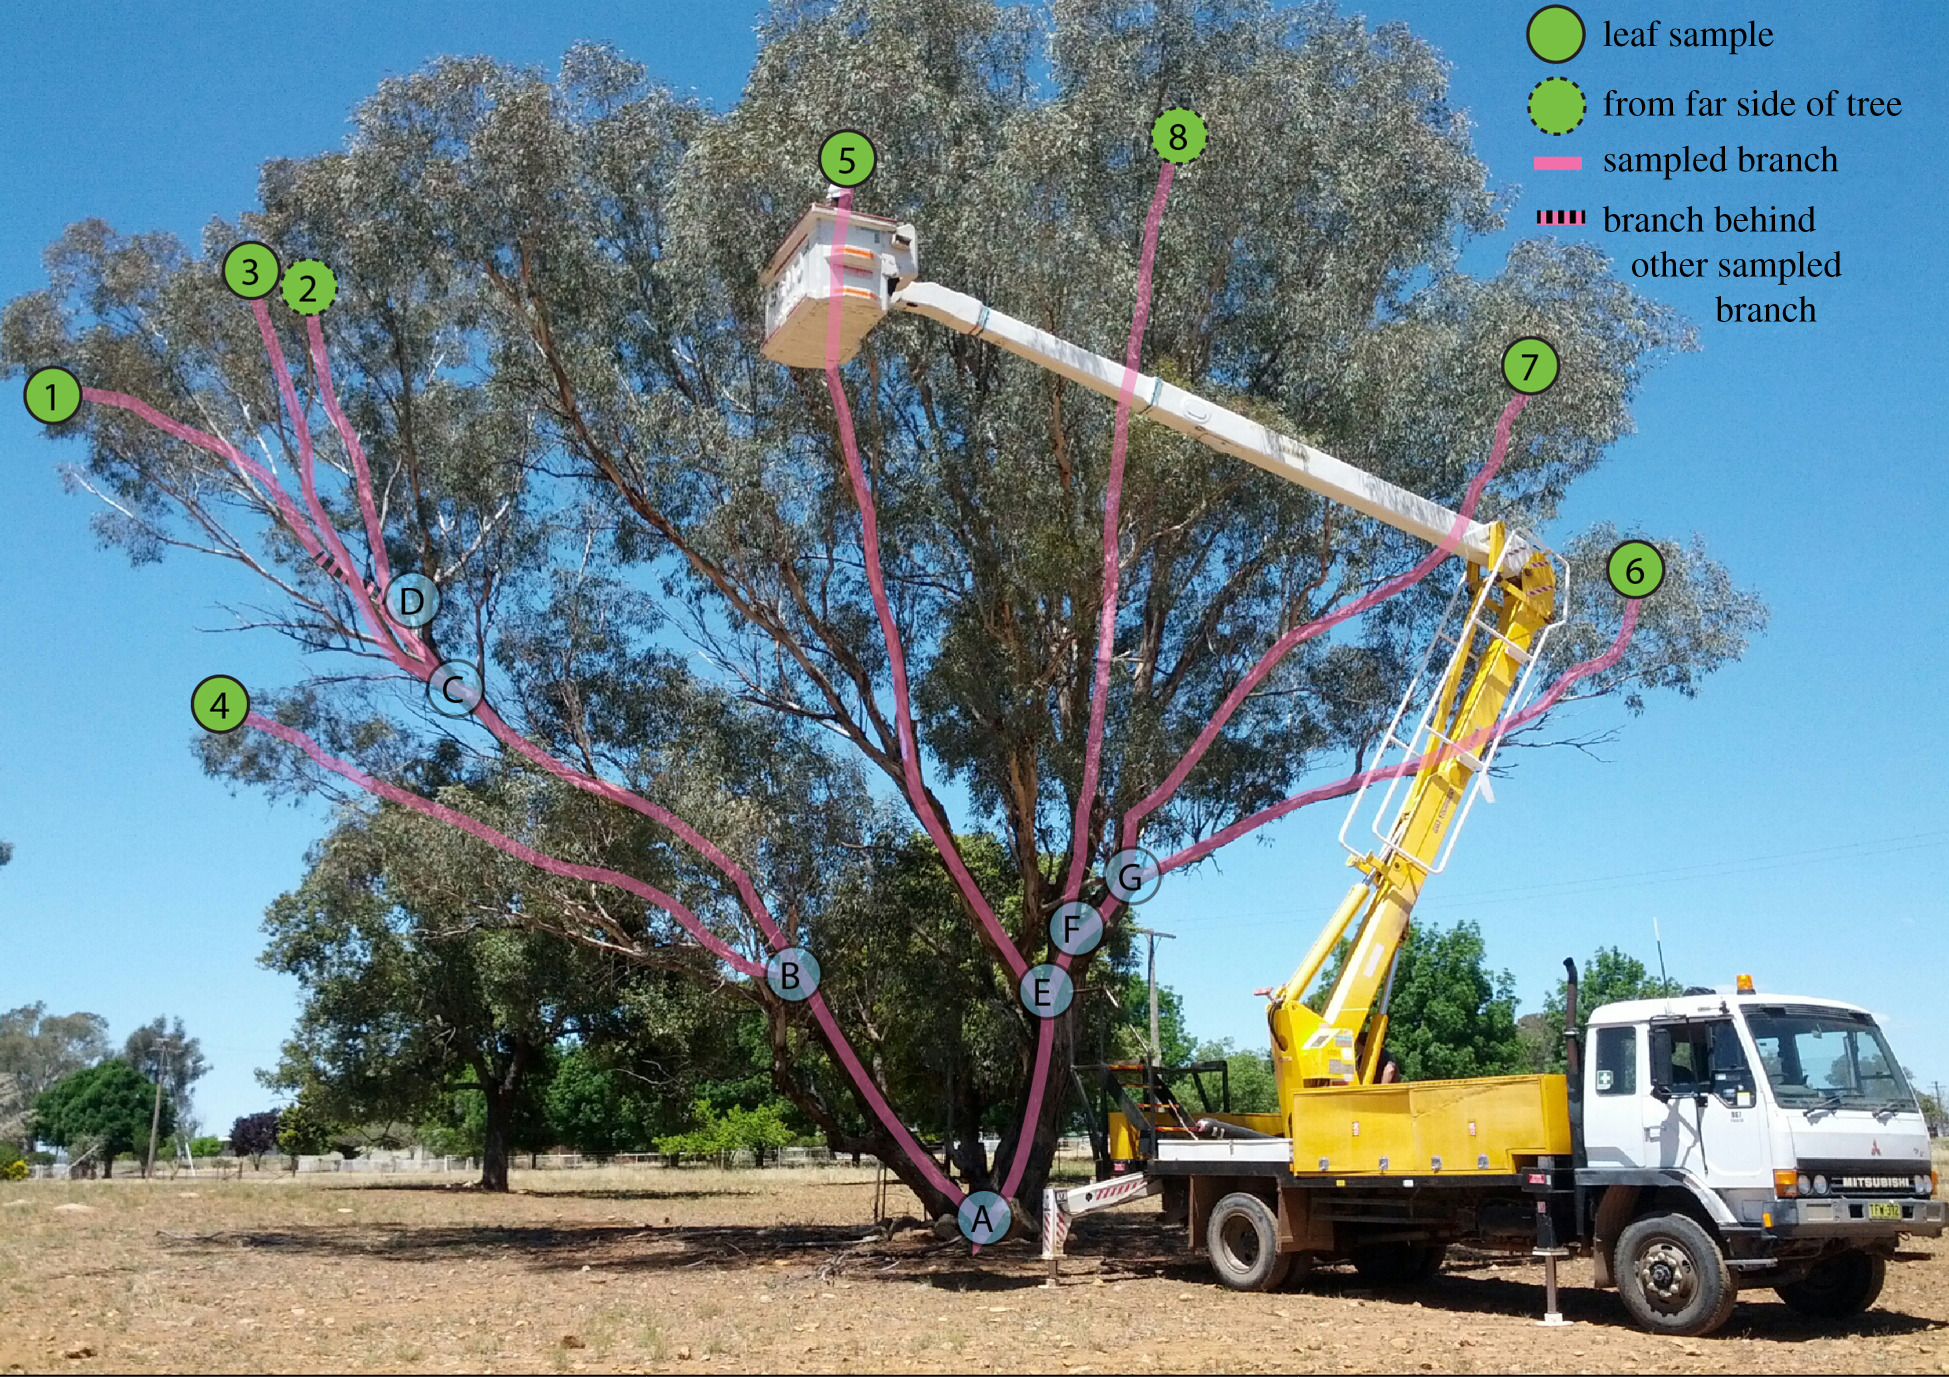
\includegraphics[width=\linewidth]{emel_1.jpg}
\titlecaption{The \textit{Eucalyptus melliodora} individual sequenced in this study}{The eight branch tips sampled are shown by numbered green circles with internal nodes of the tree shown as letters in blue circles. Circles with dashed outlines are from the far side of the tree. Pink lines trace the physical branches that connect the sampled tips. The herbivore-resistant branch comprises samples 1–3.}
\label{fig:emel_1}
\end{figure}

\subsection{DNA extraction, library preparation, and sequencing}

The branches were maintained below -80°C on dry ice and in liquid nitrogen while sub-sampled in the laboratory. From each branch, we selected a branch tip which had at least three consecutive leaves still attached to the stem. From this branch tip, we independently sub-sampled roughly 100 mg of leaf from the ‘tip-side' of the mid-vein on three consecutive leaves using a single hole punch into a labelled microcentrifuge tube containing two 3.5 mm tungsten carbide beads. The sealed tube was submerged in liquid nitrogen before the leaf material was ground in a Qiagen TissueLyser (Qiagen, Venlo, Netherlands) at 30 Hz in 30 s intervals before being submerged in liquid nitrogen again. This was repeated until the leaf tissue was a consistent powder, up to a total of 3.5 min grinding time.

DNA was extracted from this leaf powder using the Qiagen DNeasy Plant Mini Kit (Qiagen, Venlo, The Netherlands), following the manufacturer's instructions. DNA was eluted in 100 µl of elution buffer. DNA quality was assessed by gel electrophoresis (1\% agarose in 1 × TAE containing ethidium bromide), and quantity was determined by Qubit Fluorometry (Invitrogen, California, USA) following manufacturer's instructions.

We used a Bioruptor (Diagnode, Seraing (Ougrée), Belgium) to fragment 1 μg of DNA to an average size of 300 bp (35 s on ‘High', 30 s off for 35 cycles at 4°C). The fragmented DNA was purified using 1.6 × SeraMag Magnetic Beads (GE LifeSciences, Illinois, USA) following the manufacturer's instructions. We used Illumina TruSeq DNA Sample Preparation kit (Illumina Inc., California, USA) following the manufacturer's instructions to generate paired-end libraries for sequencing. These libraries were sequenced on an Illumina HiSeq 2500 (Illumina Inc., California, USA) at the Biomolecular Resource Facility at the Australian National University, Canberra.

\subsection{Creation of a pseudo-reference genome}

Since there is no available reference genome for E. melliodora, we created a pseudo-reference genome by iterative mapping and consensus calling. To do this, we first mapped all of our reads to version 2.1 of the E. grandis reference genome \parencite{bartholome_high-resolution_2015} using NGM \parencite{sedlazeck_nextgenmap_2013} and then updated the E. grandis reference genome using bcftools consensus \parencite{li_statistical_2011}. We iteratively repeated this procedure until we saw only marginal improvement in the number of unmapped reads and reads that mapped with a mapping quality of zero. The alignment originally contained 67 M unmapped reads and 311 M reads that mapped with zero mapping quality, out of a total of 1792 M reads. After the first iteration, the alignment contained 61 M unmapped reads and 349 M reads that mapped with zero mapping quality. After the last iteration, the alignment contained 59 M unmapped reads and 311 M reads that mapped with zero mapping quality. The consensus of this alignment served as the reference for all further downstream analyses.

\subsection{Variant calling for positive control}

To call variants for the positive control, we mapped each replicate of each branch tip (24 samples in total) to the final pseudo-reference genome using NGM and called genotypes using GATK 4 according to the GATK best practices workflow \parencite{auwera_fastq_2013}. This resulted in a full genome alignment of all 24 samples (three replicates of eight branches) and produced an initial set of 9,679,544 potential variable sites, a number which includes all heterozygous sites in the genome.

We then filtered variants to minimize the false-positive rate by retaining only those sites in which: (i) genotype calls were identical within all three replicates of each branch tip (see also electronic supplementary material, §1); (ii) at least one branch tip had a different genotype than the other branch tips; (iii) the site is biallelic, since multiple somatic mutations are likely to be extremely rare; (iv) the total depth across all samples is less than or equal to 500 (i.e. roughly twice the expected depth of 240×), since excessive depth is a signal of alignment issues; (v) the ExcessHet annotation was less than or equal to 40, since excessive heterozygosity at a site is a sign of genotyping errors, particularly in a site that is actually uniformly heterozygous throughout the tree but at which genotyping errors have caused a mutation to be called; and (vi) the site is not in a repetitive region determined by a lift-over of the E. grandis RepeatMasker annotation, as variation in repeat regions is often due to alignment error. This filtering produced a set of 99 high-confidence sites containing putative somatic mutations. The number of mutations that remained after the application of each filter is described in §5 of the electronic supplementary material.

\subsection{Positive control}

Using the set of 99 high-confidence putative somatic mutations, we use the Phangorn package in R \parencite{schliep_phangorn_2011} to calculate the parsimony score of all 10,395 possible phylogenetic trees of eight taxa. This estimates the number of somatic mutations that would be required to explain each of the 10,395 phylogenetic trees, using the Fitch algorithm implemented in the Phangorn package. Of these trees, three had the maximum-parsimony score of 78. One of these three trees matched the topology of the physical tree (figure \ref{fig:emel_2}). 

\begin{figure}
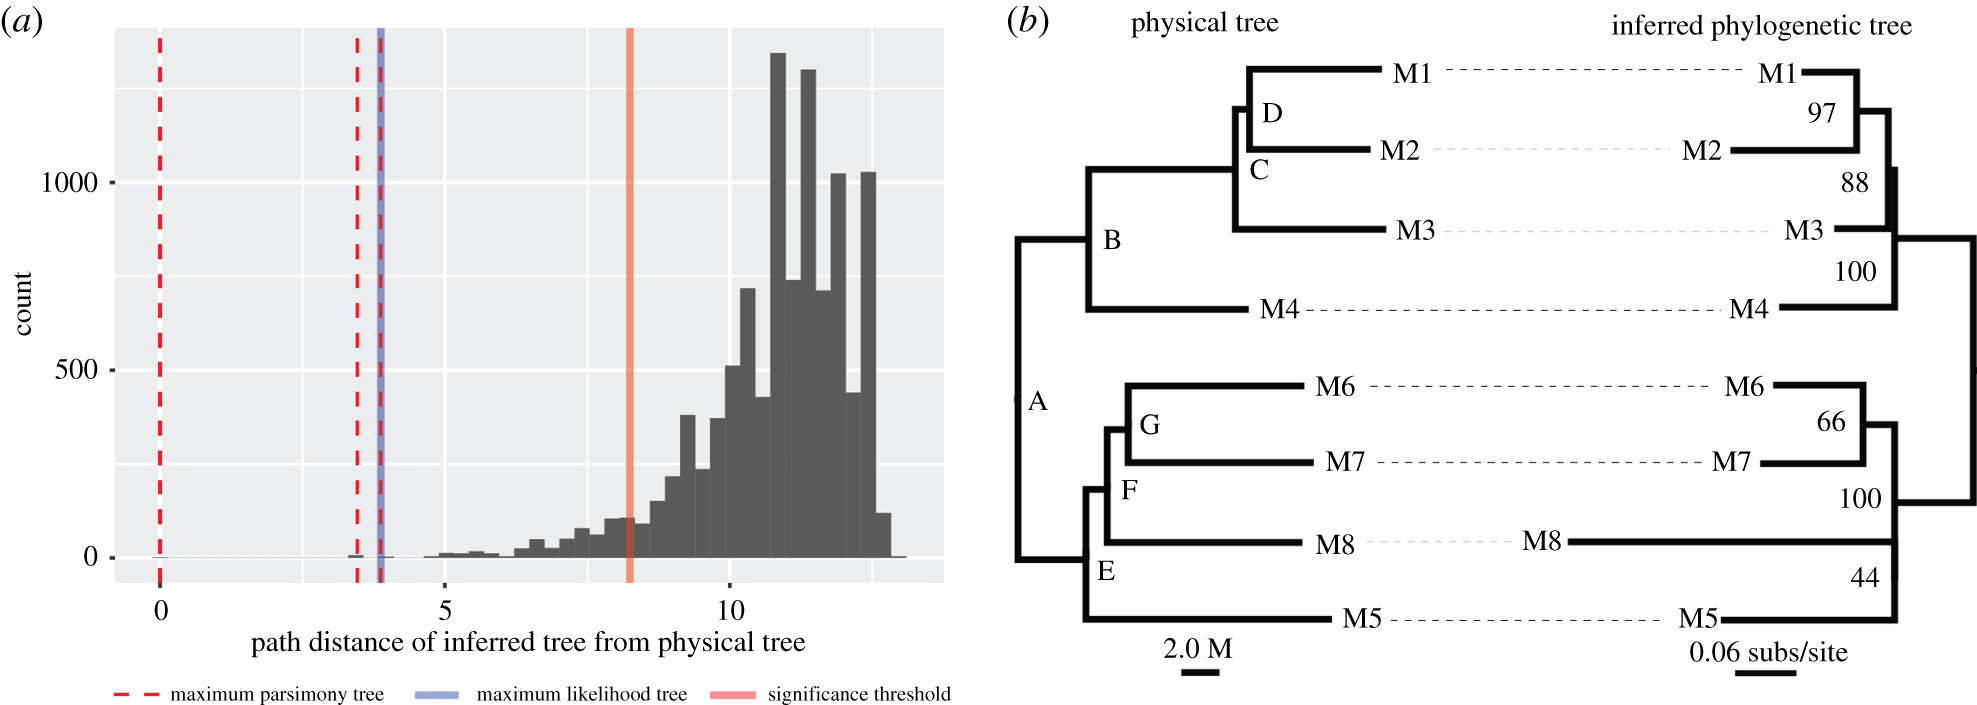
\includegraphics[width=\linewidth]{emel_2.jpg}
\titlecaption{Phylogenetic trees reconstructed from somatic mutations resemble the physical structure of the tree more closely than expected by chance}{(a) The PD between the physical tree (figure \ref{fig:emel_1}) and all 10,395 possible phylogenetic trees of eight taxa is shown as a histogram. A tree with the same topology as the physical tree will have a PD of 0. The solid red line represents the boundary of the smallest 5\% of the distribution of PDs, such that a tree with a PD lower than this line is more similar to the physical tree than expected by chance. All of the maximum-parsimony trees (dashed red lines) and the one maximum-likelihood tree (solid blue line) are more similar to the physical tree than expected by chance. (b) A side-by-side comparison of the physical tree (left, branch lengths in metres) and the maximum-likelihood tree (right, branch lengths in substitutions per site) inferred with the JC model. Letters on the nodes of the physical tree (left) correspond to the same letters of internal nodes in figure 1. Numbers on the maximum-likelihood tree (right) are bootstrap percentages. There is a single difference between the two trees: the inferred tree groups samples M8 and M5 together with low bootstrap support (44\%), which is a grouping that does not occur in the physical tree.}
\label{fig:emel_2}
\end{figure}

Next, we calculated the path difference (PD) between all 10,395 trees and the physical tree topology. The PD measures differences between two phylogenetic tree topologies \parencite{steel_distributions_1993} by comparing the differences between the path lengths of all pairs of taxa. Here we use the variant of the PD that treats all branch lengths as equal, because we are interested only in topological differences between trees, not branch length differences. Comparing all 10,395 trees to the physical tree topology provides a null distribution of PDs between all trees and the physical tree topology, which we can use to ask whether each of the three maximum-parsimony trees is more similar to the physical tree topology than would be expected by chance. To do this, we simply ask whether the PD of each of the three observed maximum-parsimony trees falls within the lower 5\% of the distribution of PDs from all 10,395 trees. This was the case for all three maximum-parsimony trees (p < 0.001 in all cases; figure \ref{fig:emel_2}), suggesting that our data contain biological signal which render the phylogenetic trees reconstructed from somatic mutations more similar than would be expected by chance to the physical tree.

\subsection{Variant calling for estimating the rate and spectrum of somatic mutations}

Using the physical tree topology to define the relationship between samples, we called somatic mutations using DeNovoGear's dng-call method \parencite{ramu_denovogear_2013} compiled from \texttt{https://github.com/denovogear/denovogear/tree/3ae70ba}. Model parameters were estimated from 3-fold degenerate sites in our NGM alignment, via VCFs generated by bcftools mpileup and bcftools call with--pval-threshold = 0. We estimated maximum-likelihood parameters using the Nelder–Mead numerical optimization algorithm implemented in the R package dfoptim (\texttt{https://cran.r-project.org/package=dfoptim}). We then called genotypes using the GATK best practices workflow as above, but with the standard-min-confidence-threshold-for-calling argument set to 0, causing the output VCF to contain every potentially variable site in the alignment. Thus, we used GATK to generate high-quality pileups from our alignments. These pileups were then analysed by dng-call to identify (i) heterozygous sites and (ii) de novo somatic mutations. Since successful haplotype construction in a region indicates a high-quality alignment, we used Whatshap 0.16 \parencite{martin_whatshap_2016} to generate haplotype blocks from the heterozygous sites.

Next, we filtered our de novo variant set to remove potential false positives. We removed variants that (i) were on a haplotype block with a size less than 500 nucleotides (among other things, this filter will remove many putative variants that fall in long repeat regions); (ii) were within 1000 nucleotides of another de novo variant (indicative of alignment issues such as might occur in repeats and other regions); (iii) had an log likelihood of the data (LLD) score less than -5 (indicative of poor model fit); and (iv) had a de novo mutation probability (DNP) score less than 0.99999 (retaining only the highest confidence variants). This produced a final variant set of 90 variants.

\subsection{Estimation of the false-negative rate}

To estimate the number of mutations that we were likely to have filtered out in our variant calling pipeline, we used the method of \cite{ness_estimate_2012}, adapted to the current phylogenetic framework. Specifically, we randomly selected 14,000 sites from the first 11 scaffolds of the pseudo-reference genome and randomly assigned 1000 of these sites to each of the 14 branches on the tree. For each of these sites, we induced \textit{in silico} mutations into the raw reads with a three-step procedure. We first estimated the observed genotype at the root using DeNovoGear call at each site. We then chose a mutant genotype by mutating one of the alleles to a randomly chosen different base using a transition/transversion ratio of 2, reflecting the observed transition/transversion ratio of eucalypts. We edited the raw reads as follows: for each mutation, we defined the samples to be mutated as all of those samples that descend from the branch on which the \textit{in silico} mutation occurred. For example, an \textit{in silico} mutation occurring on branch B → C in figure \ref{fig:emel_1} would affect all three replicates of samples 1, 2 and 3. We then edited the reads that align to the site in question to reflect the new mutation, depending on whether the reference genotype was homozygous or heterozygous. For homozygous sites, we selected the number of reads to mutate by generating a binomially distributed random number with a probability of 0.5 and a number of observations equal to the number of reads with the reference genotype. We then randomly selected that the number of reads with the reference allele to mutate to the mutant allele and edited the raw reads accordingly. For a heterozygous site, we edited the reads to replace all occurrences of the reference allele to mutant allele. The result of this procedure is the generation of a new set of raw fastq files, which now contain information on 1000 \textit{in silico} mutations for every branch in the physical tree.

\subsection{Estimation of the false-discovery rate}

To determine the false-discovery rate of the variant calling pipeline, we simulated random trees of our samples (where each of the eight branches is represented by three tips that denote the three replicates of that branch) by shuffling the tip labels until the tree had a maximal Robinson-Foulds distance from the original tree. This 24-taxon tree shares no splits with the original 24-taxon tree, so any phylogenetic information should be removed. We simulated 100 such trees and called variants using the pipeline above, but assuming that these trees were the physical tree, and ignoring any sites we had previously called as variable. Thus, any variants called by the pipeline must be false positives. We recovered 11 false positive calls over 100 simulations (i.e. 0.11 false-positive mutations per simulation), indicating our false-discovery rate is approximately 0.12\%. We calculated the false-discovery rate only once, after the details of the pipeline were finalized, to avoid overfitting our pipeline to artefactually reduce the false-discovery rate.

\section{Results and discussion}

\subsection{Field sampling and sequencing}

We selected eight branch tips that maximized the intervening physical branch length on the tree (figure \ref{fig:emel_1}), reasoning that this would increase our power by maximizing the number of sampled cell divisions and thus somatic mutations. We performed independent DNA extractions from three leaves from each branch tip, prepared three independent libraries for Illumina sequencing and sequenced each library to 10× coverage (assuming a roughly 500 Mbp genome size, as is commonly observed in \textit{Eucalyptus} species \parencite{grattapaglia_progress_2012}) using 100 bp paired-end sequencing on an Illumina HiSeq 2500. Quality control of the sequence data verified that each sample was sequenced to approximately 10× coverage and that each branch tip was therefore sequenced to approximately 30× coverage.

\subsection{Positive control analysis}

We first performed a positive control to confirm that the phylogeny of a set of high-confidence somatic variants matches the physical structure of the tree. This approach relies on being able to infer the ontogeny of the tree with sufficient accuracy that a valid comparison can be made between the ontogeny of the tree and a phylogeny generated from that tree's somatic variants. Documenting a plant's ontogeny with sufficient accuracy may not be possible for all plant species or individuals. Nevertheless, the physical structure of the tree we studied was clear (figure \ref{fig:emel_1}), and although \textit{Eucalyptus} trees are known to frequently lose branches, branch loss and regrowth should not affect the correlation between ontogeny and phylogeny provided that sufficient mutations accumulate during cell replication. To perform the phylogenetic positive control, we created a pseudo-reference genome using our data to update the genome of \textit{E. grandis} (see methods). We then called variants using GATK \parencite{mckenna_genome_2010} in all three replicates of all eight branch tips and used a set of strict filters (see methods and supplementary information) designed to avoid false-positive mutations in order to arrive at an alignment of 99 high-confidence somatic variants. To find the phylogenetic trees that best explain this alignment, we calculated the alignment's parsimony score on all 10,395 possible phylogenetic trees of eight samples. Parsimony is an appropriate method here because we do not expect more than one mutation to occur at any single site on any single branch of the \textit{E. melliodora} tree. We then asked whether the three phylogenetic trees with the most parsimonious scores were more similar to the physical structure of the tree than would be expected by chance. To do this, we calculated the PD between the structure of the physical tree and each of the three most parsimonious trees. We then compared these differences to the null distribution of PDs generated by comparing the structure of the physical tree to all possible 10,395 trees of eight samples (figure \ref{fig:emel_2}a). All three maximum-parsimony trees were significantly more similar to the physical tree than would be expected by chance (p < 0.001 in all cases; figure \ref{fig:emel_2}a, dashed red lines). Furthermore, one of the most parsimonious trees is identical to the structure of the physical tree, and a maximum-likelihood tree calculated from the same data shows just one topological difference compared to the structure of the physical tree, in which sample 8 is incorrectly placed as sister to sample 5, but with low bootstrap support of 44\% (figure \ref{fig:emel_2}a, blue line; figure \ref{fig:emel_2}b). As would be expected if plants accumulate somatic mutations as they grow, there is a significant correlation between the branch lengths of the physical tree measured in metres and the branch lengths of the maximum-parsimony tree of the same topology measured in number of somatic mutations (linear model forced through the origin: R2 = 0.82, p < 0.001; see also electronic supplementary material, §4). Notably, while various factors such as the difficulty of correctly inferring plant ontogeny may limit the utility of a phylogenetic positive control such as we present here (i.e. may produce false-negative results in which the structure of the tree appears, erroneously, to differ from the phylogeny of the sequenced genomes), it is unlikely that these factors would erroneously cause a close match between the physical structure of the tree and a phylogeny generated from the genomes of eight branches of that tree (i.e. a false positive). We therefore conclude that these analyses demonstrate that the phylogeny recovered from the genomic data matches the physical structure of the tree and confirm that there is a strong biological signal in our data.

\subsection{Estimation of the somatic mutation rate}

We next developed a full maximum-likelihood framework that extends the existing models in DeNovoGear \parencite{ramu_denovogear_2013} to detect somatic mutations in a phylogenetic context and used this framework to estimate the full rate and spectrum of somatic mutations in the individual \textit{E. melliodora} (see Material and methods). This method improves on the approach we used in our positive control, above, because it increases our power to detect true somatic mutations and avoid false positives by assuming that the phylogenetic structure of the samples follows the physical structure of the tree, an assumption that is validated by the analyses above. It also makes better use of the replicate sampling design than the method we use for our positive control, above, by directly modelling the expected variation in sequencing data across our three biological replicates under the expectation that all three replicates were sequenced from a single underlying genotype (see methods and electronic supplementary material). Using this framework, we identified 90 high-confidence somatic variants.

Of the 90 high-confidence variants we identified, 20 were in genes. Of these, six were in coding regions, with five non-synonymous mutations and one synonymous mutation. The small sample size of synonymous and non-synonymous mutations means that we cannot provide a meaningful estimate of the ratio of non-synonymous to synonymous somatic mutations, although such an estimate would help to understand the extent to which somatic mutations may be under selection. We detected seven mutations on the branch that separates the herbivore-resistant samples from the other samples (branch B → C, figure \ref{fig:emel_1}). Although we lack the functional evidence to determine whether any of these mutations are directly involved in the resistance phenotype, two of the mutations occur near genes that are plausible candidates for further investigation. One mutation occurs near Eucgr.C00081, which is a zinc-binding CCHC-type protein belonging to a small protein family known to bind RNA or ssDNA in \textit{Arabidopsis thaliana} and thus potentially involved in gene expression regulation. Another mutation occurs near Eucgr.I01302, an acid phosphatase that may have as a substrate phosphoenol pyruvate, and therefore may be involved in pathways associated with the production of various secondary metabolites, including those identified in a recent GWAS study in a closely related eucalypt \parencite{kainer_high_2019}.

We used the replicate sampling design of our analysis to estimate the false-negative rate and the false-discovery rate of our approach. It is necessary to estimate both the number of false-negative mutations and the number of false-positive mutations in order to estimate a somatic mutation rate. The former allows one to correct for the number of somatic mutations which a pipeline has failed to detect, while the latter allows one to correct for the number of somatic mutations which a pipeline has erroneously inferred. We estimated the false-negative rate by creating 14,000 \textit{in silico} somatic mutations in the raw reads \parencite{keightley_estimation_2014}, comprising 1000 \textit{in silico} mutations for each of the 14 branches of the physical tree, and measuring the recovery rate of these \textit{in silico} mutations using our maximum-likelihood approach. We were able to recover 4193 of the \textit{in silico} mutations, suggesting that our recovery rate is 29.95\%, and thus our false-negative rate is 70.05\%. This false-negative rate was similar across all of the 14 branches in the tree (see electronic supplementary material, §2). Our ability to recover mutations differs substantially between repeat regions and non-repeat regions: we recover 40\% of the simulated mutations in non-repeat regions, but just 13\% of the simulated mutations in repeat regions (which make up roughly 40\% of the genome). This difference is explained primarily by the stringent filters we use, that lead us to screen out many putative somatic mutations in repeat regions. We then estimated the number of false-positive mutations in our data, and hence the false-discovery rate (the percentage of the observed mutations that are false positives) by repeating our detection pipeline after permuting the labels of samples and replicates to remove all phylogenetic information in the data, and only considering sites that we had not previously identified as variable (see methods). By removing phylogenetic information and previously identified variable sites, we can be sure that any mutations detected by this pipeline are false positives. Across 100 such permutations, we detected 11 false-positive mutations in total, suggesting that our pipeline generates 0.11 false-positive variant calls per experiment, and that the false-discovery rate for our analysis is 0.12\%.

Based on these analyses, we can estimate the mutation rate per metre of physical growth and per year. We estimate that the true number of somatic mutations in our samples is 300 (calculated as: (90 high-confidence mutations minus 0.11 false-positive mutations)/the recovery rate of 0.2995)). Since we sampled a total of 90.1 m of physical branch length, this equates to 3.3 somatic mutations per diploid genome per metre of branch length, or $2.75 \times 10^{-9}$ somatic mutations per base per metre of physical branch length. Although the exact age of this individual is unknown and difficult to estimate---it lives in a temperate climate and does not produce growth rings---its age is nevertheless almost certainly between 50 and 200 years old. Given that the physical branch length connecting each sampled branch tip to the ground varies between 8.4 m and 20.3 m, we estimate that the mutation rate per base per year for a single apical meristem lies in the range $1.16 \times 10^{-10}$ to $1.12 \times 10^{-9}$ (i.e. $8.4 \times 2.75 \times 10^{-9}/200$ to $20.3 \times 2.75 \times 10^{-9}/50$). It is important to note that it remains unclear whether mutations in growing plants accumulate linearly with the amount of physical growth. Indeed, evidence is accumulating that in at least some (and perhaps most) species, mutations may accumulate primarily at branching events rather than during elongation of individual branches \parencite{watson_germline_2016,burian_patterns_2016}. If this is the case, then the correlation we observe between the physical branch length and the number of inferred somatic mutations (see above, and electronic supplementary material, §4) may be due to a correlation between the physical length of a branch and the number of branching events that occurred along that branch during the plant's development. It is not possible to directly estimate the number of branching events along each branch in the individual tree we used in this study, because we expect that the tree will have regularly lost branches throughout its life, leaving no accurate record of the number of branching events.

\subsection{What drives differences in somatic mutation rates among species?}

With some additional assumptions, it is also possible to estimate the mutation rate per generation and to compare this to estimates from other plants. The average height of an adult \textit{E. melliodora} individual is between 15 m and 30 m \parencite{boland_forest_2006}, so if we assume that all somatic mutations are potentially heritable (about which there is limited evidence \parencite{plomion_oak_2018} and ongoing discussion \parencite{lanfear_plants_2018}), we can estimate the per-generation mutation rate. To do this, we assume that a typical seed will be produced from a branch that has experienced 15–30 m of linear growth from the seed \parencite{boland_forest_2006}, and that mutations will have accumulated along that branch at $2.75 \times 10^{-9}$ somatic mutations per base per metre of physical branch length, estimated above. We therefore estimate that the heritable somatic mutation rate per generation is between $4.13 \times 10^{-8}$ and $8.25 \times 10^{-8}$ mutations per base. For comparison the roughly 20 cm tall \textit{Arabidopsis thaliana} has a per-generation mutation rate of $7.1 \times 10^{-9}$ mutations per base \parencite{ossowski_rate_2010}. To the extent that such a comparison is accurate, which will be somewhat limited because the former estimate considers only somatic mutations and the latter considers all heritable mutations including those caused during meiosis, we can then compare these estimates. Comparing the estimates suggests that despite being roughly 100 times taller than \textit{Arabidopsis thaliana}, the per-generation mutation rate of \textit{E. melliodora} is just approximately 10 times higher, which is achieved by a roughly fifteen-fold reduction in the mutation rate per physical metre of plant growth.

Our work adds to a growing body of evidence that low somatic mutation rates per unit of growth are a general feature of many large plant species \parencite{plomion_oak_2018, schmid-siegert_low_2017, hanlon_somatic_2019, wang_architecture_2019, bobiwash_somatic_2013}. For example, a recent study of the Sitka spruce estimated a per-generation somatic mutation rate of $2.7 \times 10^{-8}$, with confidence intervals that overlap ours \parencite{hanlon_somatic_2019}. While this per-generation rate is very similar to the one we estimate here, the rate of somatic mutation per metre of growth is around an order of magnitude lower in the Sitka spruce than our estimate for \textit{E. melliodora} ($2.75 \times 10^{-9}$ somatic mutations per base pair per metre of growth for \textit{E. melliodora} estimated here, versus $3.5 \times 10^{-10}$ somatic mutations per base pair per metre of growth for Sitka spruce, estimated by dividing the per-generation mutation rate of $2.7 \times 10^{-8}$ mutations per base by the average height of studied individuals of 76 m \parencite{hanlon_somatic_2019}, an appropriate calculation because the somatic mutation rate was estimated from paired samples taken from the base and the top of a collection of individual trees). Lower somatic mutation rates per unit of growth in larger plants may be the result of selection for reduced somatic mutation rates in response to the accumulation of increased genetic load in larger individuals \parencite{plomion_oak_2018, schmid-siegert_low_2017, lanfear_taller_2013, hanlon_somatic_2019, zhong_two_2014, klekowski_mutation_1988, scofield_definitive_2014}. This pattern could also explain why larger plants tend to have lower average rates of molecular evolution than their smaller relatives \parencite{lanfear_taller_2013, smith_rates_2008}.

Several possible mechanisms might account for a reduction in accumulation of mutations per unit of growth in larger plants. Selection may favour reduction in the mutation rate per cell division through enhanced DNA repair to reduce the lifetime mutation risk. Alternatively, it may be that the reduction in the mutation rate is due to slower cell division. For example, plant meristems contain a slowly dividing population of cells in the central zone of the apical meristem, and these cells are known to divide more slowly in trees than in smaller plants \parencite{romberger_plant_1993}. Indeed, the rate of cell division in the central zone is so low that one estimate put the total number of cell divisions per generation in large trees as low as one hundred \parencite{romberger_plant_1993}. Regardless of the underlying mechanism, the surprisingly low rates of somatic mutation in large plants reported here and elsewhere suggest an emerging picture in which there is a strong link between the somatic mutation rates and life history across the plant kingdom. Longevity and size are two aspects of plant life history likely to be of central importance to the evolution of somatic mutation rates. Larger plants may suffer from a higher accumulation of somatic mutations because of the necessity for additional cell divisions. Plants that live longer may suffer from a higher accumulation of somatic mutations because of the accumulation of DNA damage over time and/or increased cell turnover in long-lived tissues. The relative importance of these two factors may differ among clades, species, and individual tissues and is likely to also depend on the balance between DNA damage and repair between cell divisions \parencite{gao_interpreting_2016}, the accuracy of DNA replication, cell size, and the rate of cell division. We hope that the approach we describe here will help in further understanding how these and other factors contribute to the accumulation or avoidance of somatic mutations in plants.

\section{Data accessibility}

All of the bioinformatic workflows we describe here are provided in full detail in the GitHub repository available at \texttt{https://github.com/adamjorr/somatic-variation}. The raw short-read data are available online at \texttt{https://www.ncbi.nlm.nih.gov/bioproject/553104}.

\section{Authors' contributions}

R.L. conceived the study; D.K., A.P., C.K., L.B., W.F., T.H. and R.L. planned the study; A.J.O., D.K., A.M.-S., R.A.C. and R.L. involved in bioinformatic analysis; A.J.O., D.K. and R.A.C. involved in bioinformatic methods development; A.P. helped in laboratory work; A.P., D.K., C.B.-S., T.H. and J.-F.H. involved in fieldwork; R.L.wrote the paper; all authors discussed and interpreted results; All authors edited many drafts of the paper.

\section{Competing interests}

We declare we have no competing interests.

\section{Funding}

This work was supported by a Hermon-Slade grant to R.L. and an Australian Research Council Future Fellowship to R.L.

\section{Footnotes}

Electronic supplementary material is available online at \texttt{https://doi.org/10.6084/m9.figshare.c.4869747}.

© 2020 The Authors.

Published by the Royal Society under the terms of the Creative Commons Attribution License \texttt{http://creativecommons.org/licenses/by/4.0/}, which permits unrestricted use, provided the original author and source are credited.

\printbibliography{}

\chapter{Using structured data to evaluate methods of reference-free variant calling}
\label{ch:structured}

Genotyping a sample given a set of next generation sequencing reads is a common task in biology. However, genotyping accurately and sensitively is difficult due to errors in sequencing reads. This problem is exacerbated when genotyping non-model organisms because they may lack a polished annotated genome and other prior information that is sometimes used in genotyping pipelines. Once obtained, these genotypes can be used for many things; detecting selection in a population, discovering genes and alleles that affect a particular phenotype, or comparing them to another population to attempt to understand their evolutionary history.

While accurate genotype calls are important for all these uses, accurate detection of variation is difficult even with plenty of time, money, and other auxilliary resources available. Without a high-quality genome and a large number of reads, the task becomes much harder. However, several methods have been developed to call variants directly from sequencing reads, with no additional information necessary. These methods use de bruijn graphs or similar structures to create contiguous sequences representing the genome, much like assembly. They also keep track of which samples the sequences in the graph came from. Once the graph is completed, it can be traversed to find bubble-like structures in the graph. These are locations where the sequences specific to different samples diverge briefly, then come back together. This indicates the presence of a single nucleotide polymorphism (SNP) or short insertion-deletion in one of the samples. Then, the sequences that differ can be extracted from the graph and aligned to a reference, if one exists.

There are a variety of software packages that implement reference-free variant calling in this manner. One of the first developed is an extension of the Cortex assembler and is called cortex\_var. A more recent method called DiscoSNP++ was developed which doesn't require as much RAM or CPU and allows direct VCF output after mapping the predicted variants to a genome. DiscoSNP++ has recently been updated to include a tool specifically for use with RAD-seq data. Reference-free methods do not necessarily need to use de-bruijn graphs, however. The recently developed method, Kestrel, attempts to find variants without a graph and solely considers k-mer counts. %EBWT??

I previously called genotypes in the non-model organism \textit{Eucalyptus melliodora} using both out-of-the-box and custom methods to genotype leaves sampled across the tree \parencite{orr_phylogenomic_2020}. I leveraged the sample structure to estimate false positive rates for each step in the pipeline I used. When I began that work, the available reference-free methods were not sufficiently developed to call variants with the necessary accuracy I wanted to be confident in the results. Since then, the methods have undergone more development, so I was interested in whether they would work for the same data. In this chapter, I use the reference-free variant caller DiscoSNP++ and, as before, use the structure of the data to estimate the false positive rate. I also compare the output of the caller with the set of confident variants detected using the maximum likelihood approach described in \parencite{orr_phylogenomic_2020} and implemented with DeNovoGear. %todo: cite

\section{Methods}

%adapted from /storage/2017-03-15-eucalyptus/2019-12-16-supplement/filter_steps/false-positive-rate
%scripts are in /storage/2017-03-15-eucalyptus/2020-10-05-disco
To obtain variants to compare to the variant set obtained in \cite{orr_phylogenomic_2020}, I ran the DiscoSNP++ program on the raw sequencing reads. DiscoSNP++ was run with the included run\_discoSnp++.sh shell script with the -G, -T, and -R flags set along with the pseudo-reference genome from \cite{orr_phylogenomic_2020}. This enables alignment of the detected variants to the reference and creation of a VCF from the aligned haplotypes.

DiscoSNP++ was chosen as the reference-free caller to use because it was the only one that was able to be successfully installed and run on the system I used to analyze the data. Cortex uses a custom installation script that failed to properly compile the program; it could not properly link the submodules Cortex uses. Installation of Kestrel was standardized and simple, but required too much memory for this dataset. It was run with the default 4G of memory, 8G, 64G, and 256G, but crashed each time, complaining of insufficient memory. The manual gives no advice for setting this parameter.

To understand how each filtering step previously applied to this data affected the number of variants in this set, I applied 7 of 8 of these filters to the set of variants. Prior to these filters, however, I used BCFTools to remove any site which included a "." genotype, since every sample is diploid; "./." genotypes were permitted until the second to last step. The first filter only permits variants that appear on the first 11 scaffolds of the genome; these represent the chromosomes of \textit{E. melliodora}. Variants with depth > 500 were then excluded, as higher than expected depth is a signal of alignment problems. The ExcessHet annotation could not be used for filtering, as this filter is specific to GATK. I then filtered out variants within 50bp of an indel, another indicator of alignment issues. I then removed any variant that was not a biallelic SNP, as these are more likely to be errors than true mutations. Note that this makes it impossible for this pipeline to detect heterozygous to heterozygous mutations. I then removed variants that were in repetitive regions determined by a liftover of the \textit{E. grandis} RepeatMasker annotation to the pseudo-reference. Finally, I removed all sites where any set of three replicates did not have the same genotype. I then included only sites that included a mutation (\textit{ie.} not all heterozygous) to get the final set of variants.

To visualize how each filtering step affected the overall quality of the called variants, I concatenated the variants found in each step to create a FASTA alignment of sites and used RaxML with the -f a option to search for the best-scoring maximum likelihood tree, the -m ASC\_GTRGAMMA model to use a GTR mixture model with gamma distributed rate heterogeneity and correct for ascertainment bias, and the --asc-corr lewis option to use Paul Lewis' correction for ascertainment bias. Variant concatenation is not the optimal way to infer accurate phylogenies; however, for the purposes of a visual summary of the data it is sufficient.

	% false positive and false negative calls, I estimated the number of each type of variant at each step in the filtering process and evaluated how each filter affected the resulting phylogenies constructed using the obtained set of genotypes.
To evaluate the performance of this pipeline, I estimated the number of false positives and true positives were present in the reads. Since this is an empirical dataset and the the truth is not known, I had to estimate the number of true positives and false positives. To estimate the number of false positives, I randomized 100 trees that were maximally distant from the true tree and identified the number of mutations where the variants called matched the randomized replicate structure at each filtering step. This is similar to applying the second-to-last and last set of variant filters, but using the randomized tree instead of the true tree topology. Since a real mutation should follow the true structure of the tree but are unlikely to match the structure of the randomized trees, these variants are false positives. I then assumed a similar number of false positives appear when using the true tree structure, and infer the false positive rate of the calls is equal to the false positive rate calculated using the random trees.  %Since the randomized trees are all maximally distant from the true tree, a mutation called in a randomized tree should never be present in the true tree. Assuming a true mutation is consistent with only the true tree topology, I conclude that such mutations must therefore be false positives.

True positives are difficult to estimate, and the structure of the data does little to assist in identifying true variants. I therefore use the confident set of mutation calls made in \cite{orr_phylogenomic_2020} and treat them as the set of true positives. Any calls that overlap this set are therefore classified as true positives, and the number of calls that are not present in the set are classified as false negatives. Note that, as found in \cite{orr_phylogenomic_2020}, this set has an approximate false negative rate of 30\%, so it's possible that true mutations are not classified as such under this classification scheme.


\section{Results}

DiscoSnp++ emitted a total of of 1,114,434 potential variants; however, only 951,924 of these mapped to one of the first 11 scaffolds. After applying all filters, only 4 variants were ultimately detected (see Table \ref{ev_num_variants}). Before filtering, 27 of the 90 possible confident set variants were detected; after filtering, none were. Interestingly, the estimated number of false positives are very low, with an estimated 14.55 before filtering and only 2.8 after.

\begin{table}
\begin{tabularx}{\textwidth}{>{\hsize=1.5\hsize\linewidth=\hsize}X >{\hsize=.7\hsize\linewidth=\hsize}X >{\hsize=.9\hsize\linewidth=\hsize}X >{\hsize=.9\hsize\linewidth=\hsize}X}
\toprule
\textbf{Description} & \textbf{Num} & \textbf{Estimated} & \textbf{True}\\
& \textbf{Variants} & \textbf{False Positives} & \textbf{Positives} \\
\midrule
Appears in first 11 scaffolds & 951924 & 14.55 & 27\\
Total depth <= 500 & 910361 & 5.96 & 27\\
Not within 50bp of an indel & 893535 & 5.9 & 26\\
Biallelic SNPs & 815925 & 5.68 & 26\\
Outside repeat regions & 432414 & 2.8 & 20\\
All 3 replicates match & 2150 & - & 0\\
Only variable sites & 4 & - & 0\\
\bottomrule
\end{tabularx}
\titlecaption{Number of Detected Variants After Each Filtering Step}{The number of variants detected at each filtering step. Each row introduces a new filter that applies in addition to all the filters in the above rows. A description of each filter, the number of variants remaining after the filter has been applied, the estimated number of false positives present at that point in filtering, and the number of variants that overlaps the previously estimated confident set of variants. Since the last two steps include filtering based on replicate agreement, the method for estimating the number of false positives is not applicable; in the worst case, they are identical to the number of estimated false positives in step 6. True positives were estimated using the number of variants ultimately detected in the confident set described in \cite{orr_phylogenomic_2020}, which contains 90 variants.}
\label{tbl:ev_num_variants}
\end{table}

The trees inferred from the set of variants detected at each site are shown in Figure \ref{fig:ev_filtertrees}. The second to last filtering step where variants only pass filtering if they are consistent in all three replicates and the last filtering step where variants only pass filtering if there is a mutation (\textit{ie.} not all heterozygous sites of the same genotype) both yielded the same tree, as the nonvariable sites are removed in the tree construction pipeline. Each tree structure differs significantly from the true tree, and there are few examples of all three replicates neighboring one another.

	%TODO: add RF distances from each tree to the real tree ?

\begin{figure}
\centering
\begin{tabularx}{\textwidth}{ >{\hsize=.5\hsize\linewidth=\hsize}X >{\hsize=1.5\hsize\linewidth=\hsize}X | >{\hsize=.5\hsize\linewidth=\hsize}X >{\hsize=1.5\hsize\linewidth=\hsize}X }
\toprule
Filtering Step & Tree & Filtering Step & Tree \\
\midrule
First 11 Scaffolds & 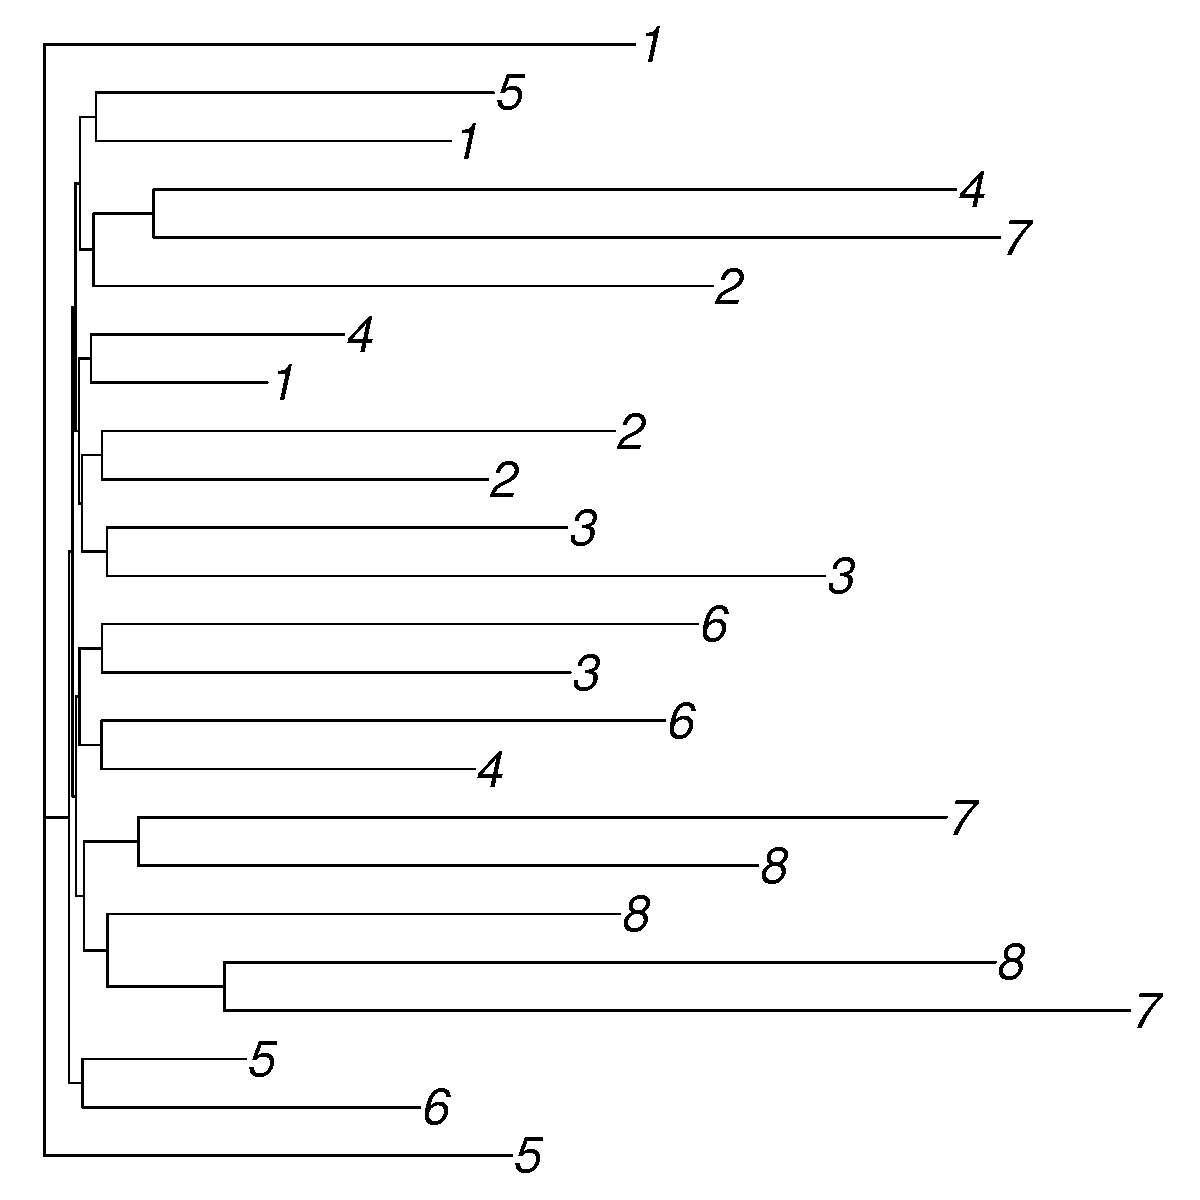
\includegraphics[width=\linewidth]{01-first-11-scaffolds.pdf} &
Depth <= 500 & 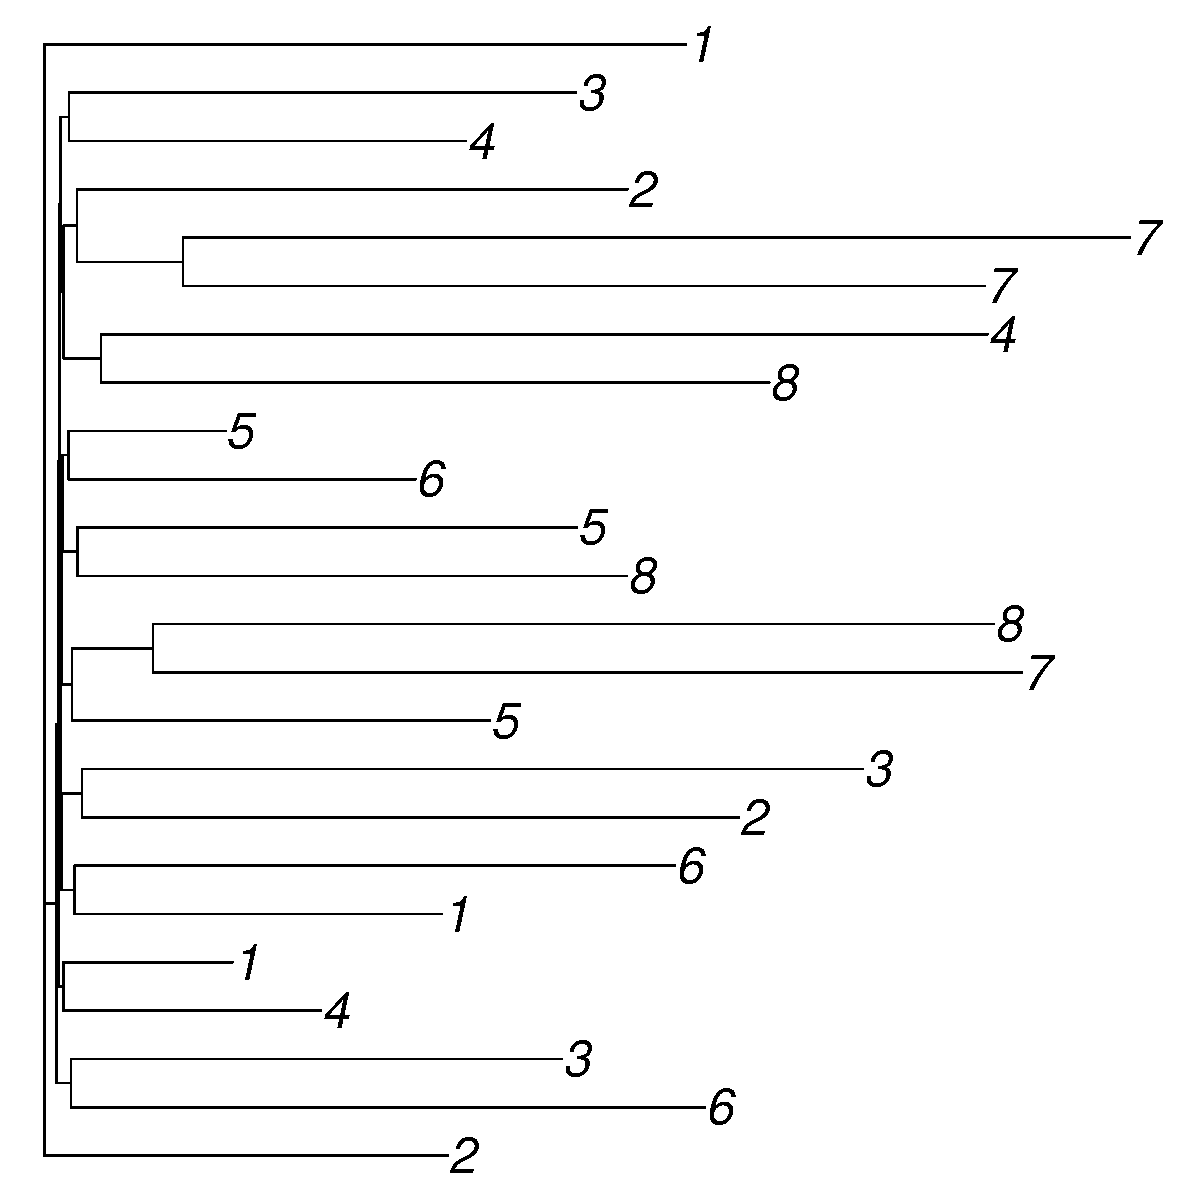
\includegraphics[width=\linewidth]{02-depth.pdf} \\
Not within 50bp of an indel & 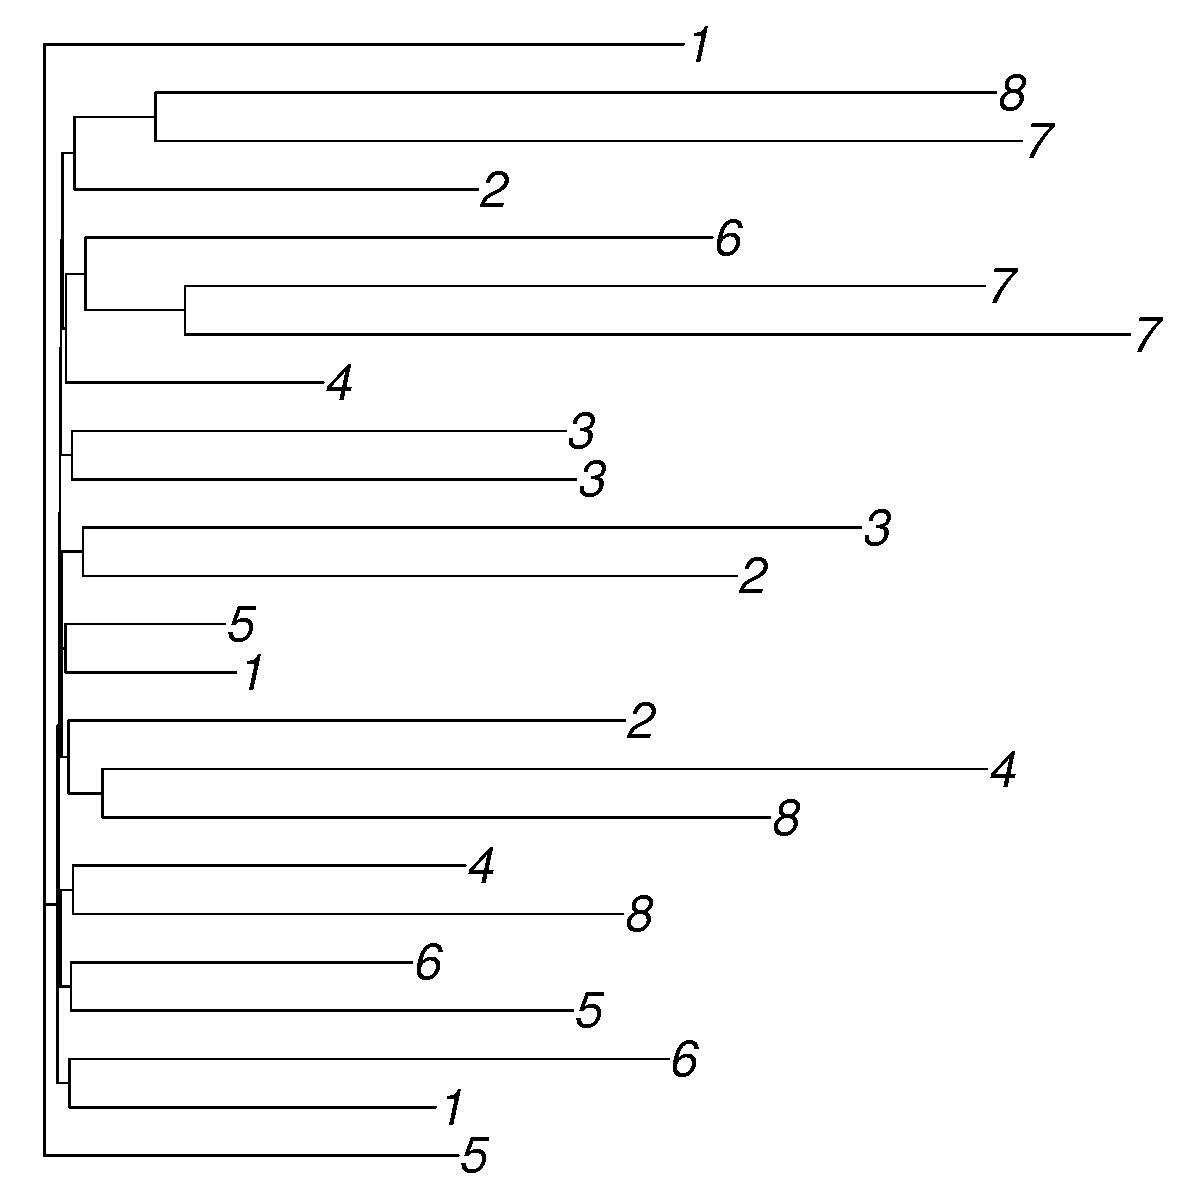
\includegraphics[width=\linewidth]{04-near-indel.pdf} &
Biallelic SNPs & 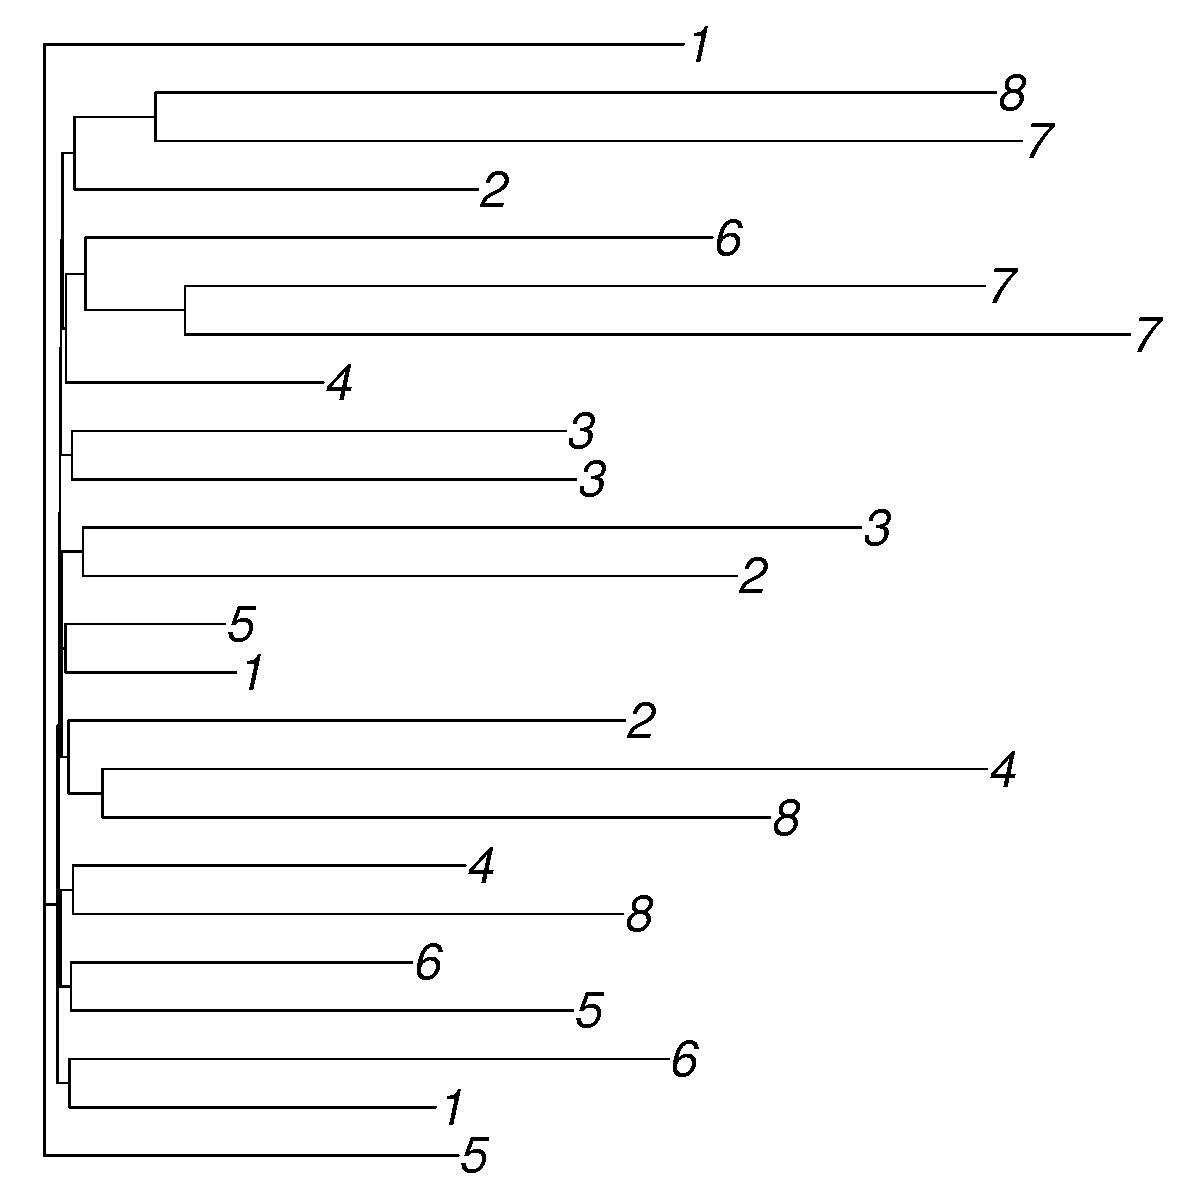
\includegraphics[width=\linewidth]{05-biallelic.pdf}\\
Outside repeat regions & 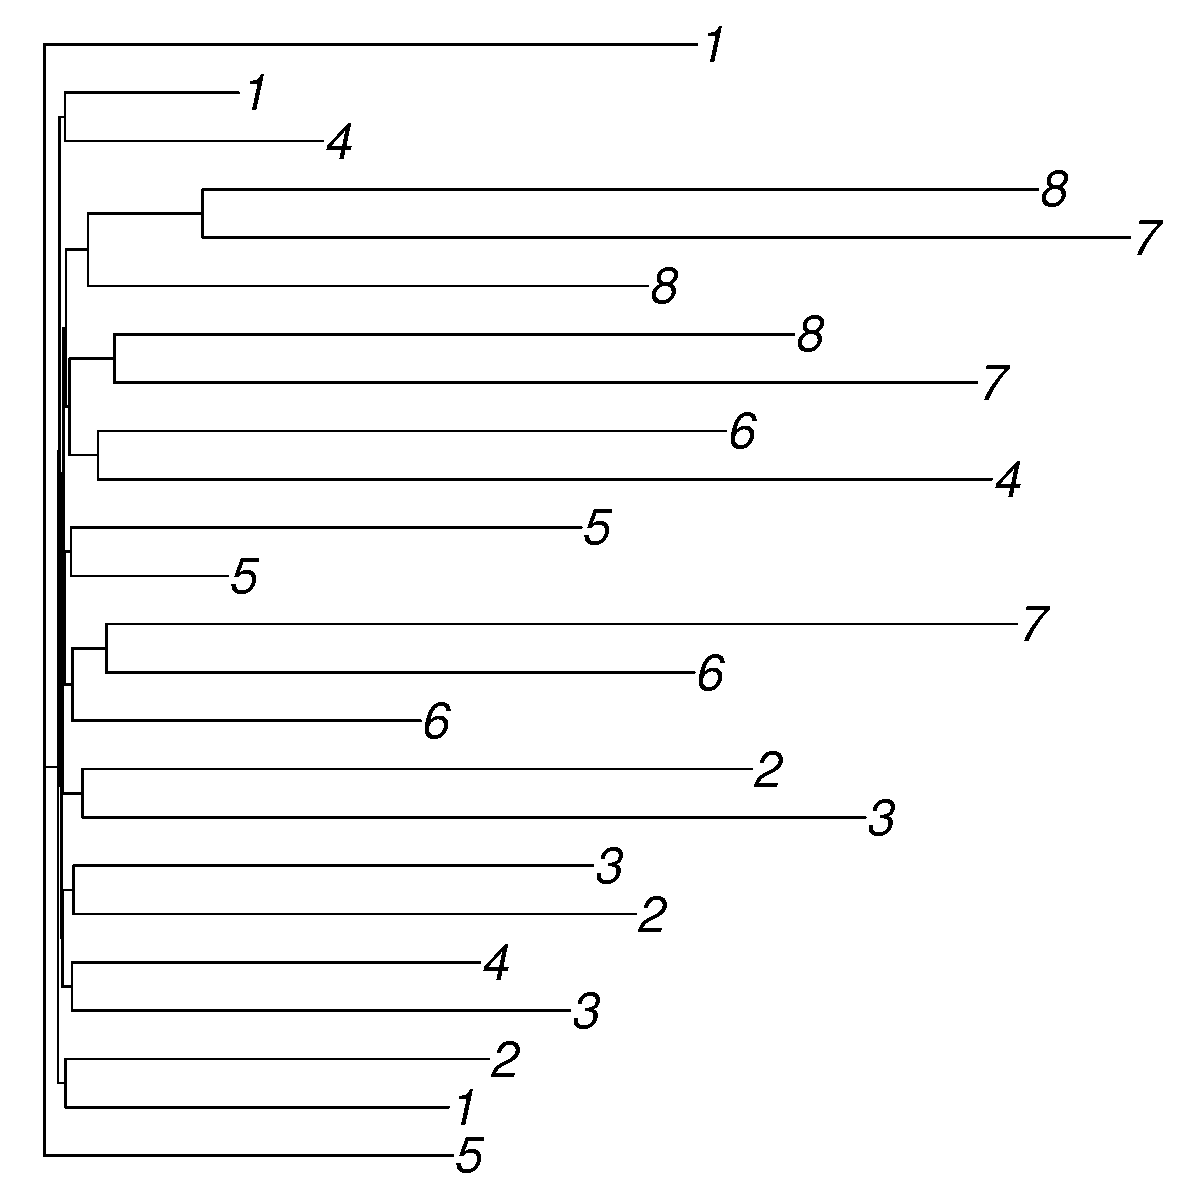
\includegraphics[width=\linewidth]{06-repeat.pdf} &
All 3 replicates match and Only variable sites & 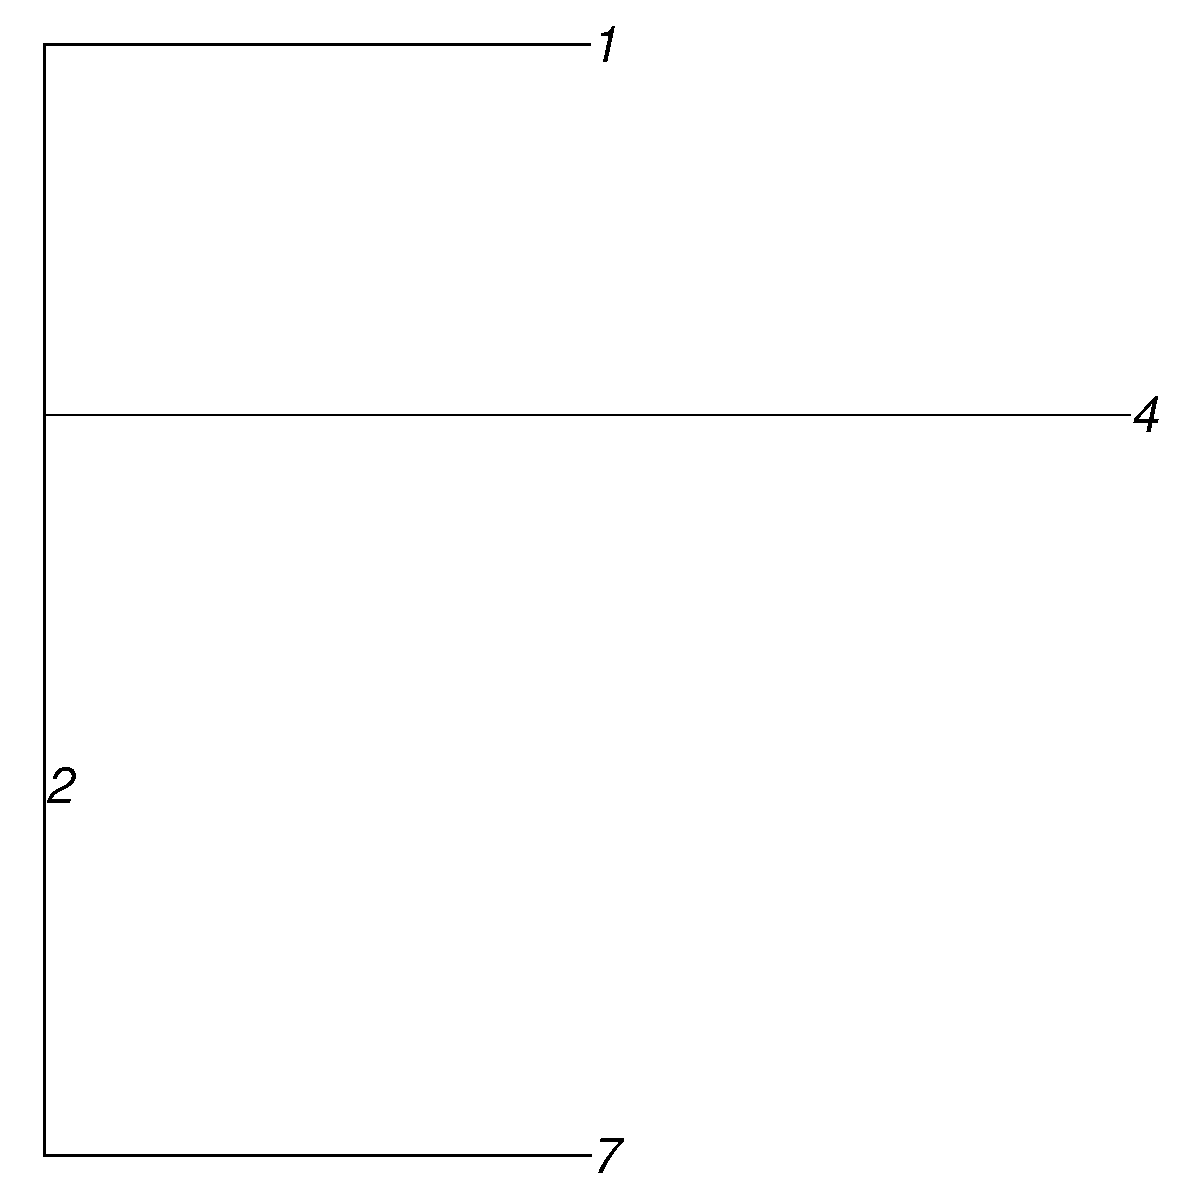
\includegraphics[width=\linewidth]{07-replicate.pdf}\\
% Only variable sites & 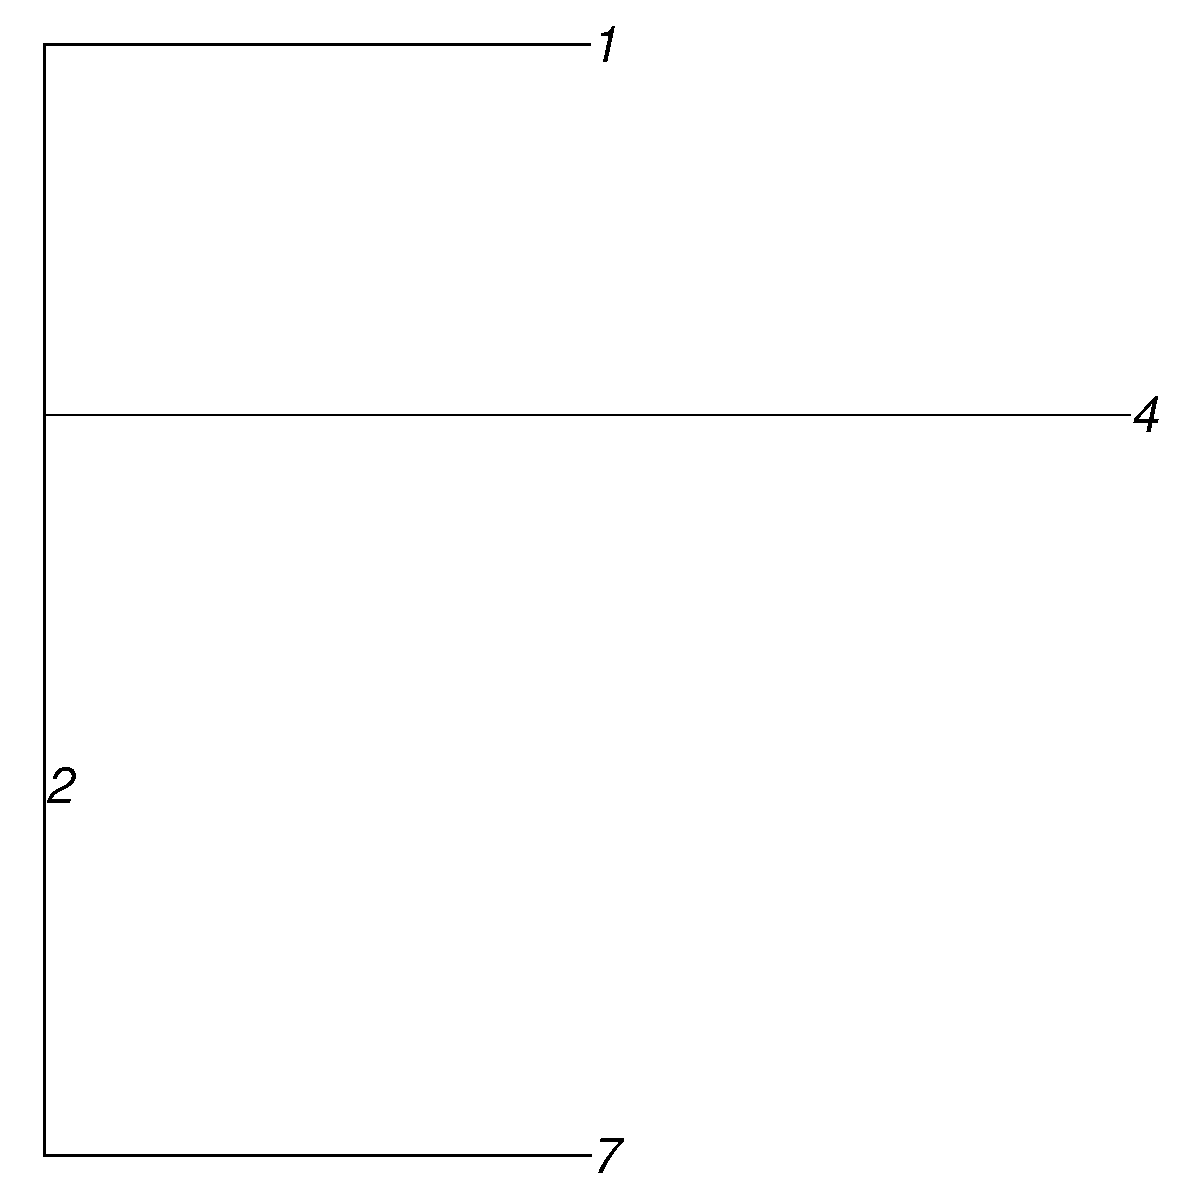
\includegraphics[width=\linewidth]{08-variable.pdf}\\
\bottomrule
\end{tabularx}
\titlecaption{Trees Inferred At Each Filtering Step}{Since each sample was derived from the branch of a tree, its genetic structure should match the physical branching structure. Thus, a phylogeny can visualize the quality of the resultant variant calls; if there are a sufficient number of true positive calls and not many false positives, the phylogeny should match the true structure.}
\label{fig:ev_filtertrees}
\end{figure}

\section{Discussion}

Unfortunately, DiscoSNP++ was not able to accurately detect mutations in this data. There are many fewer detected variants at the start of the filtering pipeline compared to those in \cite{orr_phylogenomic_2020}, with 951,924 variants on the first 11 scaffolds compared to 9,679,544 detected with HaplotypeCaller. This reduced number of potential variants is consistent throughout filtering. However, the number of estimated false positives also remains much lower, with 14.55 after the first filter is applied, in comparison to 1033.18.

At the same time, the estimated trees (Figure \ref{fig:ev_filtertrees}) show a lack of discernable signal that the variant caller is able to capture the tree structure of the data. This seems to contradict the number of false positives found at each step; if there are relatively few false positives, true mutations should drive tree construction and the trees should match the structure of the true tree---or at the very least, replicates of the same sample should be close together on the trees.

However, both tree construction and the procedure for estimating the false positive rate rely on concordance of all replicate genotypes at every site. However, the variant calls emitted by DiscoSNP++ are very sparse, with many sites having at least one missing (./.) genotype. The presence of a missing genotype for any site would eliminate the ability for it to both count as a false positive and contribute useful information during phylogeny construction. Thus, the estimate of the number of false positive sites is artificially deflated, and the number of informative sites in the alignment is small. 

	%todo: make table with number of sites that have at least 1 missing genotype
	%todo: list number of N's in each tree

There are a variety of reasons the algorithm is unable to call genotypes at so many sites. One reason is that the algorithm lacks a reference, so when it detects a variant it may not be able to map it to the genome. For complex or clustered variants, this may be a problem with some samples that doesn't also apply to other samples. This is an especially difficult problem with a repetitive and low-quality genome, such as the one used here. Another major reason is the lack of per-sample depth in this data. Since each replicate was only sequenced to 10X depth, the reads are relatively short, and the genome is repetitive, the de bruijn graph construction may not be well-connected enough to detect variant bubbles. This can very on a per-sample basis as well.

	%todo: try doing the same thing but remove replication to see how increased coverage impacts the number of calls.

\section{Conclusion}

Reference-free variant callers have the potential to be powerful tools for detecting variants in non-model organisms. They are also free of reference bias that may impact other variant callers. However, their performance leaves much to be desired in terms of speed and call accuracy. These callers likely benefit from large per-sample depths and smaller genomes with few repetitive regions. Further development of these methods is warranted.

\printbibliography

\chapter{KBBQ: A reference-free method for base quality score recalibration}
\label{ch:kbbq}
\section{Introduction}

Next generation sequencing has a plethora of applications in biology. %TODO: give some examples
While the technology is widely applied, the sequencing process is inherently erroneous and errors are common in sequencing data, with base substitution error rate estimates ranging between $.1$ and $1\%$, depending on the sequencing technology used \parencite{fox_accuracy_2014}.
To help mitigate this, DNA molecules are usually copied and sequenced multiple times to ensure the sequence is correct, since multiple independent measurements are unlikely to all contain the same error at the same position. While this works well in general, it can be costly and additional sample manipulation can damage samples and insert mutations, further increasing the amount of technical error in the data \parencite{schirmer_insight_2015, ma_analysis_2019}.

\subsection{Quality Scores}

In addition to increased sequencing depth, quality scores are an important part of sequencing data that helps identify erroneous sequences. Sequencing data is usually presented along with quality scores in the Phred scale \parencite{ewing_base-calling_1998, ewing_base-calling_1998-1}.
These quality scores measure the confidence the instrument has in its determination that any particular base in the sequence is correct.
Specifically, the quality score is equal to $-10\log_{10}P(e)$ \parencite{ewing_base-calling_1998} \parencite{ewing_base-calling_1998-1}, where $P(e)$ is the probability the base is an error.
For example, a base with a quality score of 40 has a .0001 probability of being incorrect while a base with a quality score of 10 has probability .1 of being incorrect. Generally, bases with scores lower than 10 are considered bad quality and bases with scores 30 and above are considered to be good quality. However, the score allows finer resolution than "good" and "bad", and is therefore more nuanced.

%new paragraph - importance
The usefulness of quantitative scores over categorical can be illustrated by considering how variant calling algorithms utilize quality scores.
Variant calling is a task to identify genetic variation in a sample from sequencing data.
Variant calling models use quality scores to differentially weight the observed data. Generally, these models attempt to find the sample genotype most consistent with the observed data and recognize that low quality bases provide less reliable evidence for one genotype over another. The BCFTools multiallelic caller \parencite{li_sequence_2009}, GATK's HaplotypeCaller \parencite{poplin_scaling_2018}, and FreeBayes \parencite{garrison_haplotype-based_2012}---three of the most popular variant callers---all take quality score into consideration when calling variants.
Since the quality score is an exactly defined probability, it is straightforward to integrate these scores into a model.

%new paragraph - binning
If so desired, quantitative scores can be collapsed into coarser categories, such as "good" and "bad". This is sometimes done as a heuristic; \textit{ie.} scores less than 10 are untrustworthy and filtered out of a dataset and other scores are trusted and retained.
The practice of binning quality scores together with neighboring scores is commonly performed to reduce file size \parencite{shibuya_better_2019, malysa_qvz_2015, yu_quality_2015, noauthor_reducing_2014}. 
However, it's important to note that this process cannot be simply reversed as information is lost when the scores are binned.

\subsection{Base Quality Score Recalibration}

% What is Base Quality Score Recalibration?
While base quality scores are important for identifying reliable data, base quality scores are often incorrect.
Base quality scores are exactly defined as a probability. They can be interpreted as a prediction giving the probability the reported base is an error. In general, probabilities are called \textit{calibrated} if the reported probability accurately predicts the frequency of an event.
Base quality scores in Illumina sequencing reads are not well-calibrated \parencite{callahan_dada2:_2016, ni_improvement_2016}. %(TODO: more cites)
A few alternative base calling models have been developed for Illumina machines that improve base call accuracy and quality score calibration; however, these are difficult to use because they require the raw output from the sequencing machine, which is unavailable to most users of sequencing as they are usually disposed of after a sequencing run due to the large cost associated with storing that data \parencite{kao_naivebayescall_2011, massingham_all_2012}. 


Since base quality scores are used to some degree by most variant calling methods, it is probable that poorly calibrated reads reduce the quality of resulting variant calls.
Similarly, the reduced amount of information in binned quality scores may also impact the quality of variant calls made using the data.
Poor calibration combined with poor resolution resulting from quality score binning may have an important impact on algorithms that rely on these scores to function, but the exact affect of these phenomena are unknown.

%actual BQSR
Though increased sequencing depth can help mitigate the impact of random sequencing errors, sequencing is affected by non-random biases.
For these types of errors, increasing sequencing depth counterintuitively \textit{increases} the effect of these errors, as they by definition occur preferentially at the same location. Thus, increased sequencing depth at that location adds more errors than are expected by chance, making those erroneous reads seem trustworthy. 
These biases can be due to the nature of the DNA sequence itself, with errors induced during library preparation or the sequencing reaction likely due to secondary structure \parencite{meacham_identification_2011, nakamura_sequence-specific_2011, schirmer_insight_2015, ma_analysis_2019}.
At the same time, the sequencing reaction is also non-randomly biased. Bases at the end of a read are much more likely to be erroneous than bases at the beginning of the read, and the identity of the base and adjacent bases also affect the error rate \parencite{fox_accuracy_2014, schirmer_illumina_2016}. 
Thus while random errors are troublesome, their impacts can be somewhat mitigated by more sequencing. Systematic errors cannot addressed in the same way, but they can be modeled and incorporated into quality scores.
%discuss non-random genomic locus vs. sequencing characteristics etc.    %non-random errors

% GATK BQSR occurs in 3 phases.
% Phase 1 - Count errors and covariates
Base quality score recalibration (BQSR) is the process of modeling errors in sequencing data and using the created model to update quality scores such that they reflect an accurate probability of error of any base.
GATK BQSR  is the most popular method for BQSR and is recommended before variant calling by the GATK best practices \parencite{auwera_fastq_2013}.
The model integrates many covariates of error such that the output quality score reflects an accurate, independent measure of the probability of error.
The algorithm takes reads aligned to a reference and a database of potentially variable sites in the genome as input.

The algorithm proceeds in 3 phases.
In the first phase, the algorithm compares each read to the aligned reference. Potentially variable sites are ignored and mismatches from the reference sequence and non-mismatches are counted. The numbers of matching and mismatching bases are categorized according to the model covariates, which are: read group, assigned quality score, sequencing cycle, and the base identity along with the identity of the previous base (the base context).
% Phase 2 - Train a hierarchical model.
In the second phase, a bayesian hierarchical model is trained with the count data. Using a normal distribution of the mean probability of error as a prior, the \textit{maximum a posteriori} (MAP) quality score of the read group is calculated assuming the errors are binomially distributed. The estimated error probability for each read group $\hat{Q}_{rg}$ can be written in terms of the binomial probability mass function $\mathcal{B}$ with error probability $Q_{rg}$ and number of observations $\operatorname{Observations}_{rg}$ and the normal probability density function $\mathcal{N}$ with standard deviation of 1 around the mean estimate of the quality score for the entire dataset, $\bar{Q}$
\begin{align}
\hat{Q}_{rg} &= \operatorname{argmax}_{Q_{rg}} P(Q_{rg}|\operatorname{Errors}_{rg}) \\
&= \operatorname{argmax}_{Q_{rg}} P(\mathcal{B}(\operatorname{Errors}_{rg} | \operatorname{Observations}_{rg}, Q_{rg}) \times P(\mathcal{N}(Q_{rg} | \bar{Q}))
\end{align}
This score is then used as the prior for calculating the \textit{maximum a posteriori} quality score for each assigned quality score in that read group, $\hat{Q}_{\operatorname{assigned\:quality\:score}}$, using a simular formula.
In turn, this score is used as the prior for calculating the \textit{maximum a posteriori} scores for the sequencing cycle and context covariates of bases with that score. The difference between the MAP estimate and the prior is used to calculate the final score, which is the sum of the MAP estimate of the assigned quality score and these two differences. That is,
\begin{align}
\Delta Q_{\operatorname{cycle}} &= \hat{Q}_{\operatorname{cycle}} - \hat{Q}_{\operatorname{assigned\:quality\:score}} \\
\Delta Q_{\operatorname{context}} &= \hat{Q}_{\operatorname{context}} - \hat{Q}_{\operatorname{assigned\:quality\:score}} \\
Q_{\operatorname{recalibrated}} &= \hat{Q}_{\operatorname{assigned\:quality\:score}} + \Delta Q_{\operatorname{cycle}} + \Delta Q_{\operatorname{context}}
\end{align}
In the third phase, the quality score of each read is adjusted based on the four covariates for each base in the read according to values calculated in the previous phase. See Figure \ref{fig:recal_explain} for a visual example.

\begin{figure}
\centering
	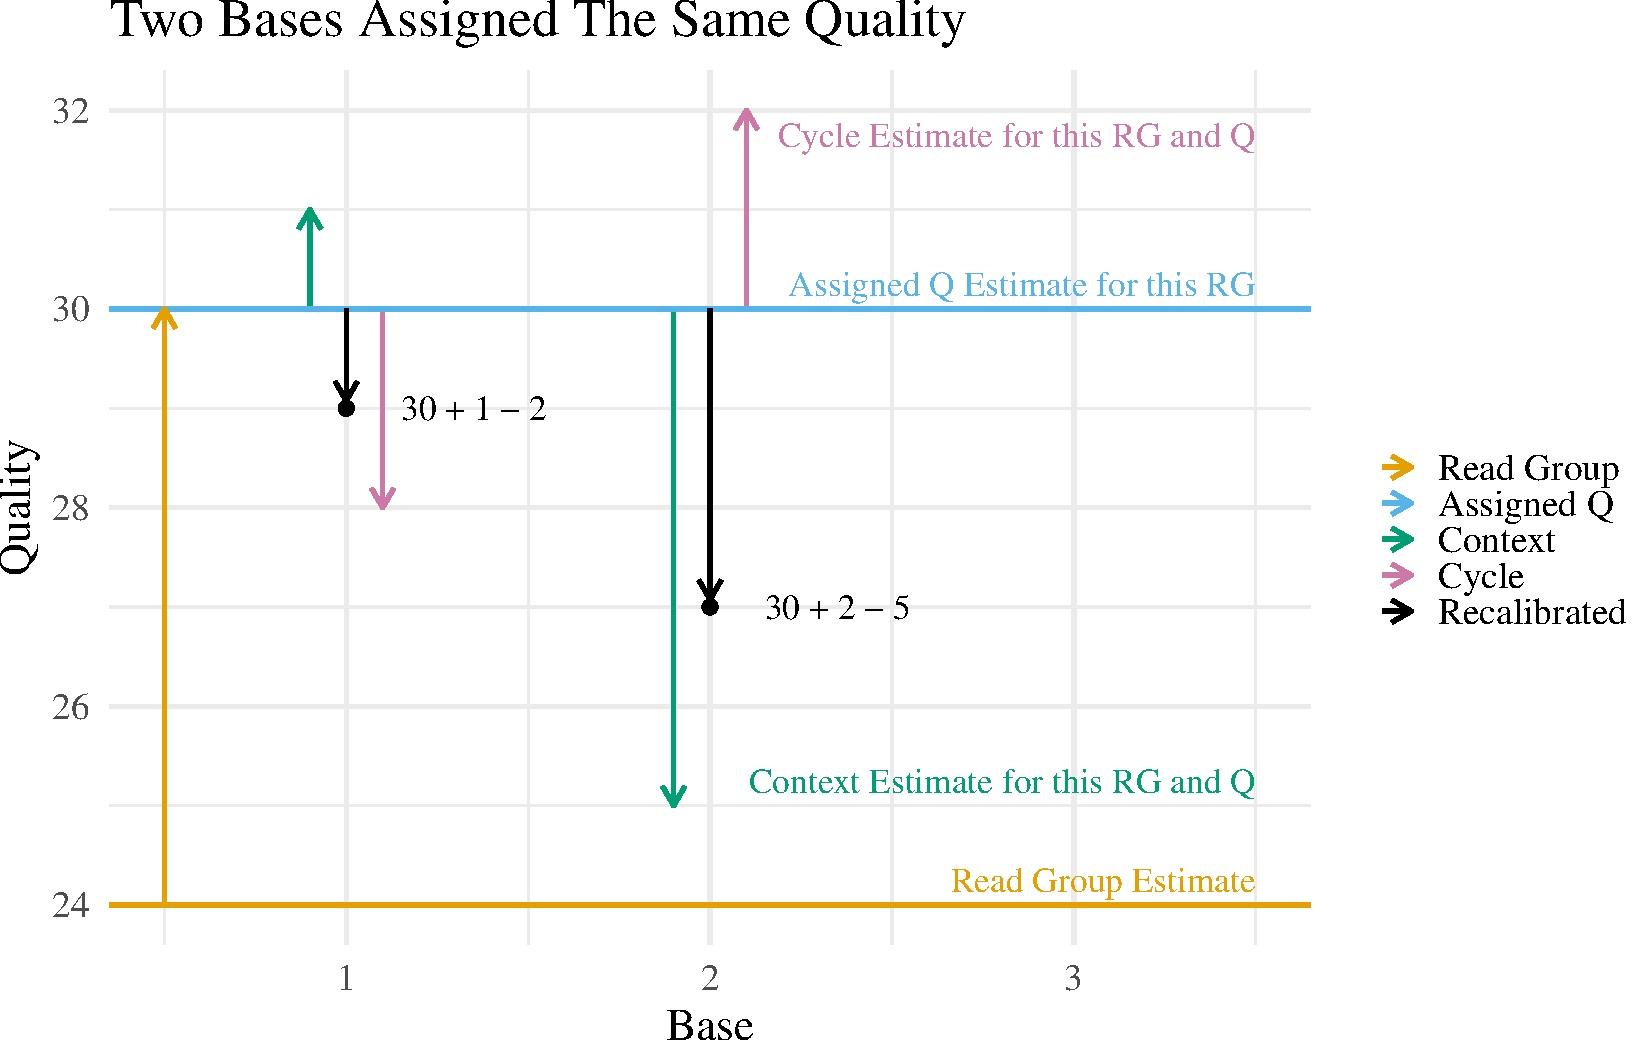
\includegraphics[width = \textwidth]{recalibration_explainer.pdf}
	\titlecaption{Base Quality Score Recalibration Example}{An example of two bases that were assigned identical quality scores. Here, the read group has an estimated quality of 24 and the assigned quality score in that read group has an estimated quality of 30. The estimated quality of bases with the same context as the first base is 31 while the estimated quality of bases with the same cycle is 28. This results in an overall estimated quality score of 29. Despite having the same read group and assigned score, because of the difference in context and cycle the second base is assigned a different score.}
	\label{fig:recal_explain}
\end{figure}


% How much does BQSR help?
BQSR improves quality score calibration in many cases, especially when there is moderate sequencing depth and the database of variable sites is nearly complete. %todo : cite
While BQSR is recommended in GATK's Best Practices, its affect on the resulting variant calls is not well-characterized, and there is ongoing debate about whether to continue recommending BQSR. \parencite{van_der_auwera_geraldine_2020, van_der_auwera_geraldine_2020_b}
However, \cite{ni_improvement_2016} find that improved quality score calibration aids detection of minor alleles in high coverage datasets by increasing sensitivity and reducing the number of false positive calls.
Thus, the need to perform BQSR and the performance of GATK's BQSR algorithm may vary from study to study.
One objective of this work is to help elucidate when GATK BQSR performs well and when it fails, and provide a method that works in situations that GATK BQSR struggles with.
As an example, the GATK developers recommend BQSR for use in cancer variant discovery \parencite{cibulskis_sensitive_2013}, but the tumor genome is likely much different from the human genome, and the database of variable sites will likely miss many truly variable sites due to the large mutation rate present in cancer genomes. Additionally, mismatches in reads misaligned due to chromosomal rearrangements may be mistakenly counted as evidence of sequencing error. The number of these errors required to significantly impact the performance of the algorithm is not clear.

\subsection{Alternate Approaches for BQSR}
% What is the problem with current methods for BQSR?
As illustrated above, the most problematic aspect of GATK BQSR occurs in the first phase of the algorithm: counting erroneous and non-erroneous bases. This is especially true when considering non-model organisms, where alignment errors may be common. Furthermore, in non-model organisms a database of variable sites is likely unavailable or largely incomplete. However, there are methods that attempt to overcome this deficiency. While there exist alternative approaches that implement different error models such as Lacer \parencite{chung_lacer:_2017}, the biggest problem for analyzing data without reliable reference information is the method of counting erroneous and non-erroneous bases.
% \item In a variant calling context, BQSR is probably most helpful in regions with low coverage, as the limited amount of data makes it difficult to differentiate between errors, heterozygous sites, and mutations.
 % or inconsistent coverage, as one may expect when sequencing a non-model organism; however, by definition that means no quality reference nor database of variable sites are available. Since these are required to perform GATK's BQSR, that means BQSR cannot be confidently completed.
% \item Find some estimates of differences between reference and samples sequenced; perhaps look at mouse
% \item This will be highly species-dependent and situation specific

% Alternative Approaches
Many alternative algorithms have been developed to avoid providing a database of variable sites. However, these approaches all still require a reference and alignment, and many require extra reagents and sequencing spike-ins that increase the cost of analysis and cannot be used to reanalyze existing sequencing data that hasn't been specially prepared.
% \item Lacer \parencite{chung_lacer:_2017} bins aligned bases based on depth and whether the base matches the reference, then uses singular value decomposition to infer the shift in quality score for each base.
ReQON \parencite{cabanski_reqon:_2012}, like GATK, considers bases that do not match the reference as errors but limits the number of acceptable errors at a position to minimize the effect of unknown variants. It then uses a logistic regression to recalibrate the quality scores.
SOAP2 \parencite{li_soap2:_2009} contains a model for consensus sequence construction that performs BQSR during construction. %It doesn't seem possible to get these recalibrated scores out??
The methods of \cite{zook_synthetic_2012} and \cite{ni_improvement_2016} use synthetic spike-ins of known composition and GATK's model \parencite{zook_synthetic_2012} or piecewise regression \parencite{ni_improvement_2016} to recalibrate quality scores. Since the sequence of the spike-in is known before hand, errors are easy to identify as there should be no biological variation in the spiked-in sample.
% \item While these approaches are useful alternatives to GATK, the comparisons presented here will only compare against GATK BQSR as none of the alternative approaches function without a reference and GATK BQSR is the most popular method.
Crucially, these methods require a reference and possibly other information to recalibrate reads that may not be available.

% kbbq
To effectively recalibrate base quality scores with as little auxiliary information as possible, I present \texttt{kbbq}, a software package to recalibrate quality scores of whole genome sequencing data without a reference or database of variable sites. The only required input is the set of reads to be recalibrated. Rather than excluding variation and comparing to the reference like GATK does, \texttt{kbbq} uses k-mer subsampling to find likely errors. Once the number of errors and nonerrors are counted and categorized according to their covariates, it uses the same model GATK uses to recalibrate the reads. Here, I show that this difference in how \texttt{kbbq} and GATK detect sequencing errors impacts the resultant base quality scores and that \texttt{kbbq} produces superior calibrations in a variety of scenarios.

\section{Methods}
	% \item Error correction algorithms
\texttt{kbbq} performs BQSR by adjusting how errors in the dataset are discovered.
Instead of looking at the reference, \texttt{kbbq} implements the error-correction algorithm described in \cite{song_lighter_2014} and uses the errors detected by that procedure to train and apply the standard GATK model. Note that the sequenced bases are not actually changed; the detected errors are used only to train the model. If there is evidence according to the model that the base is erroneous, its base quality will be decreased according to the strength of that evidence.

Briefly, the algorithm subsamples k-mers from the dataset. Since erroneous k-mers are expected to be unique, erroneous k-mers are less likely to be sampled than error-free k-mers. A binomial test is then conducted for every nucleotide in the dataset; if a sufficient number of k-mers contain the nucleotide, the base is likely not erroneous and called trusted. If \textit{k} of these trusted bases appear next to each other, that k-mer is stored as a trusted k-mer. Once the trusted k-mers have all been stored, each read is iterated through once again and any bases on the edge of an island of trusted k-mers are changed such that the change produces the maximal number of trusted k-mers in the read. These changes are marked as errors and used to train the model.
The model training and recalibration procedure are the same as those described above for GATK's BQSR method.

\subsection{KBBQ Program Input and Parameters}

\texttt{kbbq} requires as input a set of reads in FASTQ \parencite{cock_sanger_2010} or BAM \parencite{li_sequence_2009} format. If the input data is FASTQ formatted and consists of multiple read groups, the read group each read belongs to should be annotated in the name of each read. Alternatively, if the user has an original data file and a data file that has already been corrected using an error correction program, the user may supply the corrected file with the \texttt{-\phantom{}-fixed} option to obtain errors from that correction rather than performing the error correction algorithm included in \texttt{kbbq}. The program's only required parameter is the approximate length of the sequenced region in base-pairs, and this information can be taken from the BAM header if it is present. It may be set with the \texttt{-\phantom{}-genomelen} option. If BAM input is provided, the \texttt{-\phantom{}-set-oq} and \texttt{-\phantom{}-use-oq} flags can be used to set the OQ flag on the read before recalibrating or to use the quality scores encoded in the OQ flag rather than the quality scores in the primary quality score field.

Optionally, the approximate sequencing coverage may also be provided with the \texttt{-\phantom{}-coverage} option. If it is not, it will be estimated by finding the length of the sequenced data divided by the provided genome length; $\operatorname{Coverage} = \frac{\operatorname{Sequence\:Length}}{\operatorname{Genome\:Length}}$.
An $\alpha$ parameter may also be provided with the \texttt{-\phantom{}-alpha} option; this is the same $\alpha$ parameter that Lighter uses, and is the fraction of reads sampled from the input data \parencite{song_lighter_2014}. If not provided, the recommended value of $\alpha = \frac{7}{\operatorname{Coverage}}$ is used.
A $\texttt{-k}$ parameter may also be provided, which changes the k-mer size used for the error detection algorithm. The maximum value of 32 is recommended and is the default value.
A summary of flags and options the program supports is listed in table \ref{table:params}.

%new para
The genome length parameter, in addition to being used to estimate sequencing coverage, is also used to estimate the number of k-mers that will be sampled. This is used to parameterize the bloom filter that stores the sampled and trusted k-mers. This parameterization is different than that used in Lighter; there, the number of sampled k-mers is estimated to be $1.5 \times \operatorname{Genome\:length}$. However, the expected number of sampled k-mers $K_{\operatorname{sampled}}$ is bounded by the expected value of the binomial distribution parameterized by $\operatorname{Genome\:length} \times \operatorname{Coverage}$ and $\alpha$. Assuming \textit{every} k-mer is unique, the number of possible k-mers in the dataset $K_{\operatorname{total}}$ is less than $\operatorname{Coverage} \times \operatorname{Genome\:length}$. Since the number of k-mers in each read is $\operatorname{Read\:length} - k + 1$ and assuming equal read lengths, the total number of k-mers is:
\begin{align}
K_{\operatorname{total}} &= \sum_{\operatorname{Reads}}{\operatorname{Read\:length} - k + 1} \\
&= (\operatorname{Read\:length} - k + 1) \times \operatorname{Number\:of\:reads} \\
&< \operatorname{Read\:length} \times \operatorname{Number\:of\:reads} \\
&< \operatorname{Read\:length} \times \frac{\operatorname{Coverage} \times \operatorname{Genome\:length}}{\operatorname{Read\:length}} \\
&< \operatorname{Coverage} \times \operatorname{Genome\:length}
\end{align}

So the expected number of sampled k-mers is

\begin{align}
E[K_{\operatorname{sampled}}] &= E[\mathcal{B}(x; \alpha, K_{\operatorname{total}})] \\
&= \alpha \times K_{\operatorname{total}} \\
&< \alpha \times \operatorname{Coverage} \times \operatorname{Genome\:length}
\end{align}

Notably, if $\alpha$ is the recommended value of $\frac{7}{\operatorname{Coverage}}$, the expected number of sampled k-mers is less than $7 \times \operatorname{Genome\:length}$, a bound over 4 times larger than the estimate used by Lighter. For the data analyzed here, this provides a much better estimate of the true number of sampled k-mers. Ultimately, the larger estimate of elements inserted into the bloom filter causes an increase in size of the bloom filter but a smaller false positive rate.

\begin{table}
\centering
\begin{tabularx}{\textwidth}{ l  l >{\hsize=.7\hsize\linewidth=\hsize}X >{\hsize=1.3\hsize\linewidth=\hsize}X }
\toprule
\textbf{Parameter} & \textbf{Short Option} & \textbf{Default Value} & \textbf{Summary} \\
\midrule
\texttt{-\phantom{}-ksize} & \texttt{-k} & 32 & Size of k-mer to use for correction\\
\texttt{-\phantom{}-use-oq} & \texttt{-u} & Off & Use BAM OQ tag values as quality scores\\
\texttt{-\phantom{}-set-oq} & \texttt{-s} & Off & Set BAM OQ tag values before recalibration\\
\texttt{-\phantom{}-genomelen} & \texttt{-g} & Estimated for BAM, required for FASTQ & The approximate size of the sequenced region in base-pairs.\\
\texttt{-\phantom{}-coverage} & \texttt{-c} & Estimated from data & Approximate sequencing coverage\\
\texttt{-\phantom{}-fixed} & \texttt{-f} & Off & Treat changes to reads in the given file as errors and recalibrate. \\
\texttt{-\phantom{}-alpha} & \texttt{-a} & 7 / coverage & Rate to sample k-mers\\
\texttt{-\phantom{}-threads} & \texttt{-t} & 1 & Number of CPU threads to use\\
\bottomrule
\end{tabularx}
\titlecaption{KBBQ Parameters}{Provides the short options for each long parameter name, the default value of the parameter and a summary of how each parameter changes the behavior of the program.}
\label{table:params}
\end{table}

\subsection{Testing and Validation}
% Describe test dataset used for benchmarking.
To test the performance of \texttt{kbbq}, I reanalyzed the synthetic diploid CHM1-CHM13 dataset from \cite{li_synthetic-diploid_2018}. Like other benchmarking datasets, this dataset includes a BED file describing confident regions in which the genotype of any site that differs from homozygous reference within those regions are included in a VCF file. For the purposes of this work, I assume these confident regions and associated VCF entries are correct and represent the true genotype of the sequenced sample.

This dataset was specifically designed to study the impact of deep sequencing on variant calling and has a coverage of approximately 45x. Thus, the affect of sequence specific errors and other non-random biases in sequencing should be pronounced in this data.
The dataset was constructed by adding equal concentrations of DNA of CHM1 and CHM13 human complete hydatidiform mole cell lines and sequencing the mixture. These moles are formed when a sperm combines with an egg containing no nucleus; the sperm then undergoes mitosis to generate a completely homozygous cell mass. They are effectively haploid, and it is significantly easier to genotype a haploid cell than a diploid one. Thus, the mixture simulates a diploid human cell but the genotype of each haplotype is known. This means there should be very few, if any, errors in the declared genotypes included with the data. This is what \cite{li_synthetic-diploid_2018} find when validating their data as well.

%new paragraph
To measure the performance of \texttt{kbbq} and compare to GATK's BaseRecalibrator and ApplyBQSR tools, I subset the full dataset to only reads aligned on Chromosome 1 and overlapping the BED of confident regions using the samtools view command \parencite{li_sequence_2009}. I then used the samtools fixmate and view commands to remove any singleton reads. I then ran \texttt{kbbq} on the dataset with the options \texttt{-\phantom{}-use-oq -g 214206308 -a .15}. I also ran GATK's BaseRecalibrator with the provided variant data as the known sites file and the \texttt{-\phantom{}-use-original-qualities} flag set. I then used the ApplyBQSR tool with the \texttt{-\phantom{}-use-original-qualities} flag to recalibrate the input file. The \texttt{-\phantom{}-use-original-qualities} flag is appropriate here because the data has already been recalibrated and the original assigned quality scores are stored in the OQ tag on each of the reads. This flag tells GATK to use and recalibrate those quality scores, rather than using the scores that are already present in the QUAL field for the read.

I then compared the two recalibrated files by running the BaseRecalibrator tool again on both output datasets. In this invocation of BaseRecalibrator, \texttt{-\phantom{}-use-original-qualities} was not set as the quality scores in the QUAL field of the recalibrated reads are the quality scores calculated using the models trained above. I then used GATK's AnalyzeCovariates tool to create CSV files containing the number of errors for each assigned quality scores and plotted these values.

% Subsampling of database of variable sites - move this to Ch5
In order to determine how misspecification of the database of variable sites affects the calibration of GATK's BQSR procedure, I simulated datasets with various levels of false negative and false positive variants. In this case, false negative variants in the database of variable sites causes a site that should be ignored to not be ignored, greatly increasing the number of bases that GATK classifies as sequencing errors. On the other hand, false positive variants remove a site from GATK classification, so the affect is likely to be small except for large false positive rates. To create each false negative dataset, an appropriate number of sites from the VCF were randomly sampled with BCFTools and the shuf program. To create each false positive dataset, all sites from the VCF were extracted in BED format with the BCFTools query command, then subtracted from the BED of confident regions with bedtools subtract \parencite{quinlan_bedtools_2010}. The appropriate number of sites were then sampled with the shuf program and appended to the sites from the VCF to generate the BED file of all sites to exclude. These files were then provided as input to GATK's BaseRecalibrator tool and calibration was evaluated with GATK's AnalyzeCovariates tool.

% GATK chimp test
To simulate a situation where a researcher has sequenced a non-model organism, is using a reference that may not closely match the sample, and doesn't have a database of variable sites, I aligned the test data to the chimp reference genome \parencite{waterson_initial_2005} using NextGenMap \parencite{sedlazeck_nextgenmap_2013}. Prior to realignment, the original qualities in the OQ tag were placed into the QUAL field using GATK's RevertBaseQualityScores tool to ensure the raw assigned quality scores were used to align the reads.

In this situation, GATK recommends calling an initial set variants with high confidence and using these variants as the database of variable sites. %todo: give GATK parameters, etc used.
To see how this affects the results of GATK's BQSR, I called variants using HaplotypeCaller with the \texttt{-stand-call-conf 50} argument. The default value for this argument is 40, and is a phred-scaled confidence threshold for reporting a variant, so with this flag the model's confidence in the emitted calls should be very high. I then used the resulting variants as the database of variable sites with BaseRecalibrator to train a recalibration model. Here, the \texttt{-\phantom{}-use-original-qualities} flag was not used as the qualities in the QUAL field for each read were already the raw uncalibrated scores.

To evaluate this model using the truth set, I used the model and ApplyBQSR to recalibrate the reads as they were aligned to the human reference. Here, the \texttt{-\phantom{}-use-original-qualities} flag was used, as the quality scores that represent the original assigned scores for the reads (the same scores used to train the model) are given in the OQ tag rather than the QUAL field. Since the recalibration was performed after the reads were already aligned to the human reference, the sole difference between this recalibration method and the standard using the correct reference and database of variable sites is the trained model; the alignment has no impact on benchmarking the calibration. I then used AnalyzeCovariates as above to obtain the calibration data and plot it.

% Simulated Reads
As an additional test of KBBQ's performance, particularly in situations where the user has no quality reference, I simulated reads from the unscaffolded contigs of the initial release (v1.0) of the \textit{Eucalyptus grandis} genome, SRA accession AUSX00000000.1. GATK recommends using at least 100 million base pairs for calibration, so I aimed to simulate twice that many bases. To simulate a situation where a user has a medium-coverage dataset of approximately 20X coverage, I therefore simulated a haploid genome of 5 million base pairs by randomly sampling contigs from the full set of \textit{E. grandis} contigs using shuf, awk, and the samtools faidx program.

I then simulated heterozygous sites in the genome using simuG \parencite{yue_simug_2019} with a transition/transversion ratio of 2 to mirror the approximate ratio of mutations in real eucalypts. I simulated 125,000 SNPs in the reference to reflect the large level of heterozygosity in eucalypts \parencite{kulheim_comparative_2009}. I then concatenated the subsampled reference and reference containing the SNPs, which I used to simulate 101-bp long paired end reads using ART \parencite{huang_art_2012} using the HiSeq 2500 error profile, a mean fragment length of 300, a fragment length standard deviation of 20, and a depth of coverage of 20. Since this concatenated genome is twice the size as the haploid genome, at 20 fold coverage it would yeild approximately 200 million base-pairs of sequence. I then aligned the simulated reads to the genome with NextGenMap \parencite{sedlazeck_nextgenmap_2013}.

This reflects a scenario where a researcher sequences a highly heterozygous individual, assembles contigs, and aligns the sequenced reads back to the assembly. However, in this case the locations of all heterozygous sites are known. To compare the performance of KBBQ and GATK recalibration, I built the recalibration model with GATK BaseRecalibrator using the true location of all the heterozygous sites and applied the model with with GATK ApplyBQSR, both without the \texttt{-\phantom{}-use-original-qualities} flag since the assigned quality scores were present in the QUAL field of the read. Since most researchers don't have knowledge of all the true variable sites in the data, I also repeated this procedure but using the initial calls made by HaplotypeCaller with the \texttt{-\phantom{}-stand-call-conf} parameter set to 50, which makes HaplotypeCaller emit only variants it is highly confident in. I then ran KBBQ using a k-mer size of 32 and a genome length of 5 million to recalibrate the reads. Finally, I used BaseRecalibrator again and GATK's AnalyzeCovariates tool with the CSV output option to check the calibration of each of the four recalibrated alignments.

%

Scripts to replicate the above analyses are available in Appendix \ref{ch:kbbq_plot_code}.

\section{Results}
To identify how errors in the database of variable sites affects calibration, I simulated different datasets with known false positive rates, plotted the calibration and calculated the root mean squared error (RMSE) of the data recalibrated with the model trained using each database as the known sites input to GATK BaseRecalibrator. These plots are shown in figure \ref{figure:fpr}, and the RMSE of the quality score for each dataset is shown in table \ref{table:fpr}. For all these datasets, the false negative rate is 0. As the false positive rate increases, the degree of miscalibration doesn't change significantly except for the 100\% false positive rate dataset, which is very poorly calibrated; however, this calibration is likely an artifact (see section \ref{sec:kbbq_discussion}).

\begin{figure}
\centering
	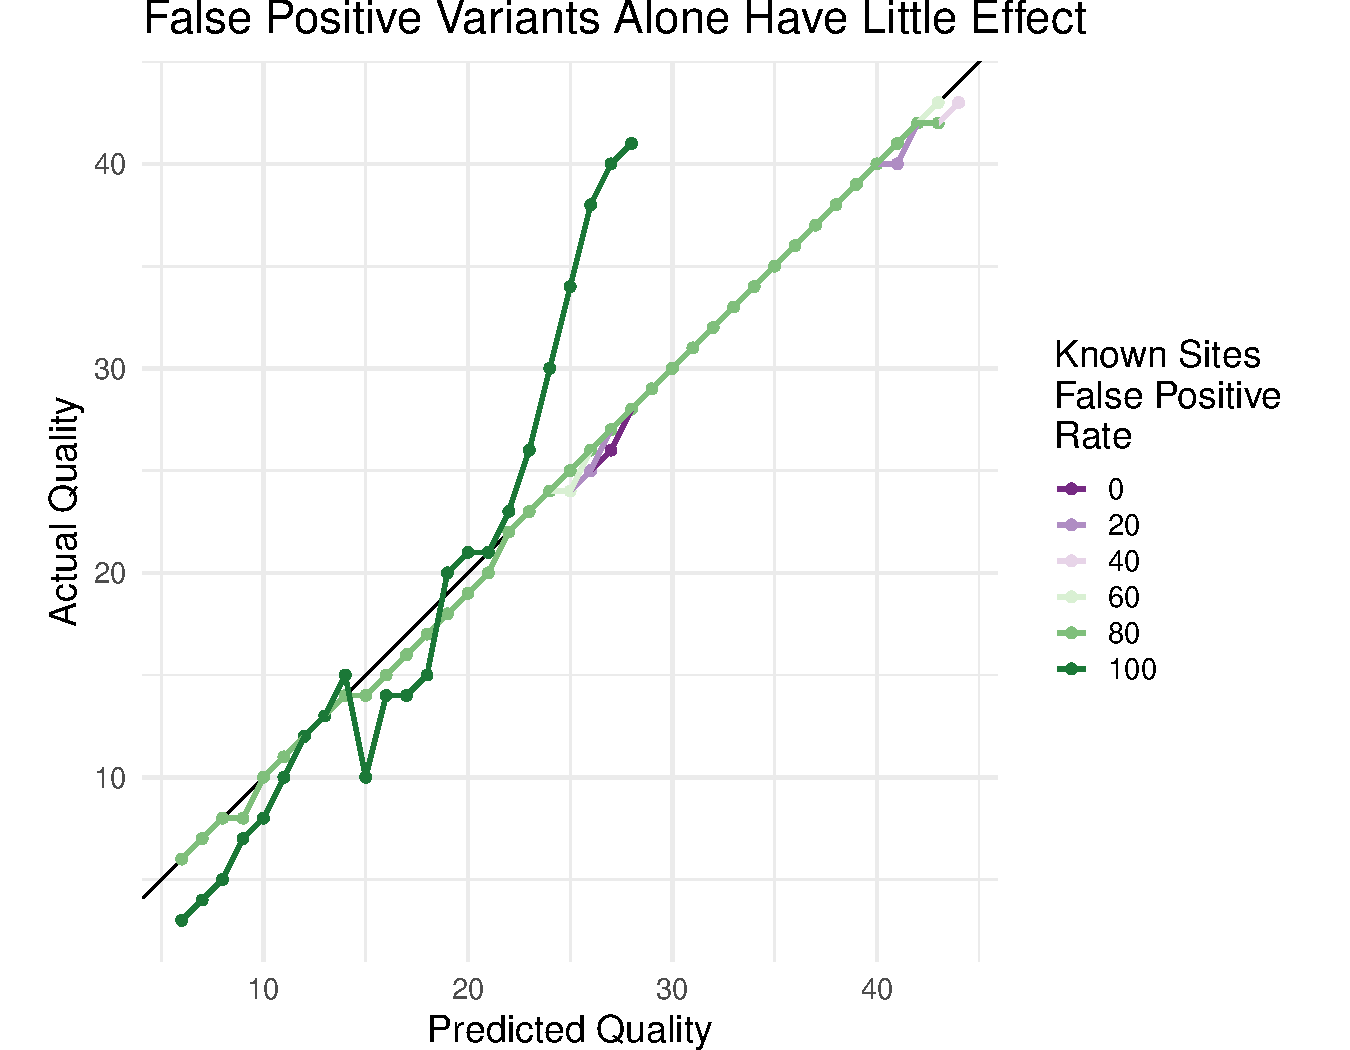
\includegraphics[width = .6\textwidth]{fpr.pdf}
	\titlecaption{False Positive Only Calibration}{Base quality score calibration for a range of false positives in the database of variable sites. The false negative rate for all datasets is zero. Increasing the false positive rate does not significantly impact the quality of the calibration. The poor calibration at a 100\% false negative rate is likely an artifact (see Section \ref{sec:kbbq_discussion}).}
	\label{figure:fpr}
\end{figure}

\begin{table}
\centering
\begin{tabular}{r l}
\toprule
False Positive Rate & RMSE \\
\midrule
0 & 0.60 \\
20 & 0.58 \\
40 & 0.53 \\
60 & 0.49 \\
80 & 0.49 \\
100 & 5.50 \\
\bottomrule
\end{tabular}
\titlecaption{False Positive Calibration Errors}{The root mean squared error of quality score for reads recalibrated using a database of variable sites with different false positive rates. The false negative rate for each dataset is 0\%.}
\label{table:fpr}
\end{table}

I also simulated different databases of variable sites with differing false negative rates and similarly used it to recalibrate the CHM1-CHM13 data. In these datasets, the false positive rate is 0\%. The plotted calibration and RMSE of the recalibrated data is shown in figure \ref{figure:fnr} and table \ref{table:fnr}. As the false negative rate increases, the degree of miscalibration also steadily increases.

\begin{figure}
	\centering
	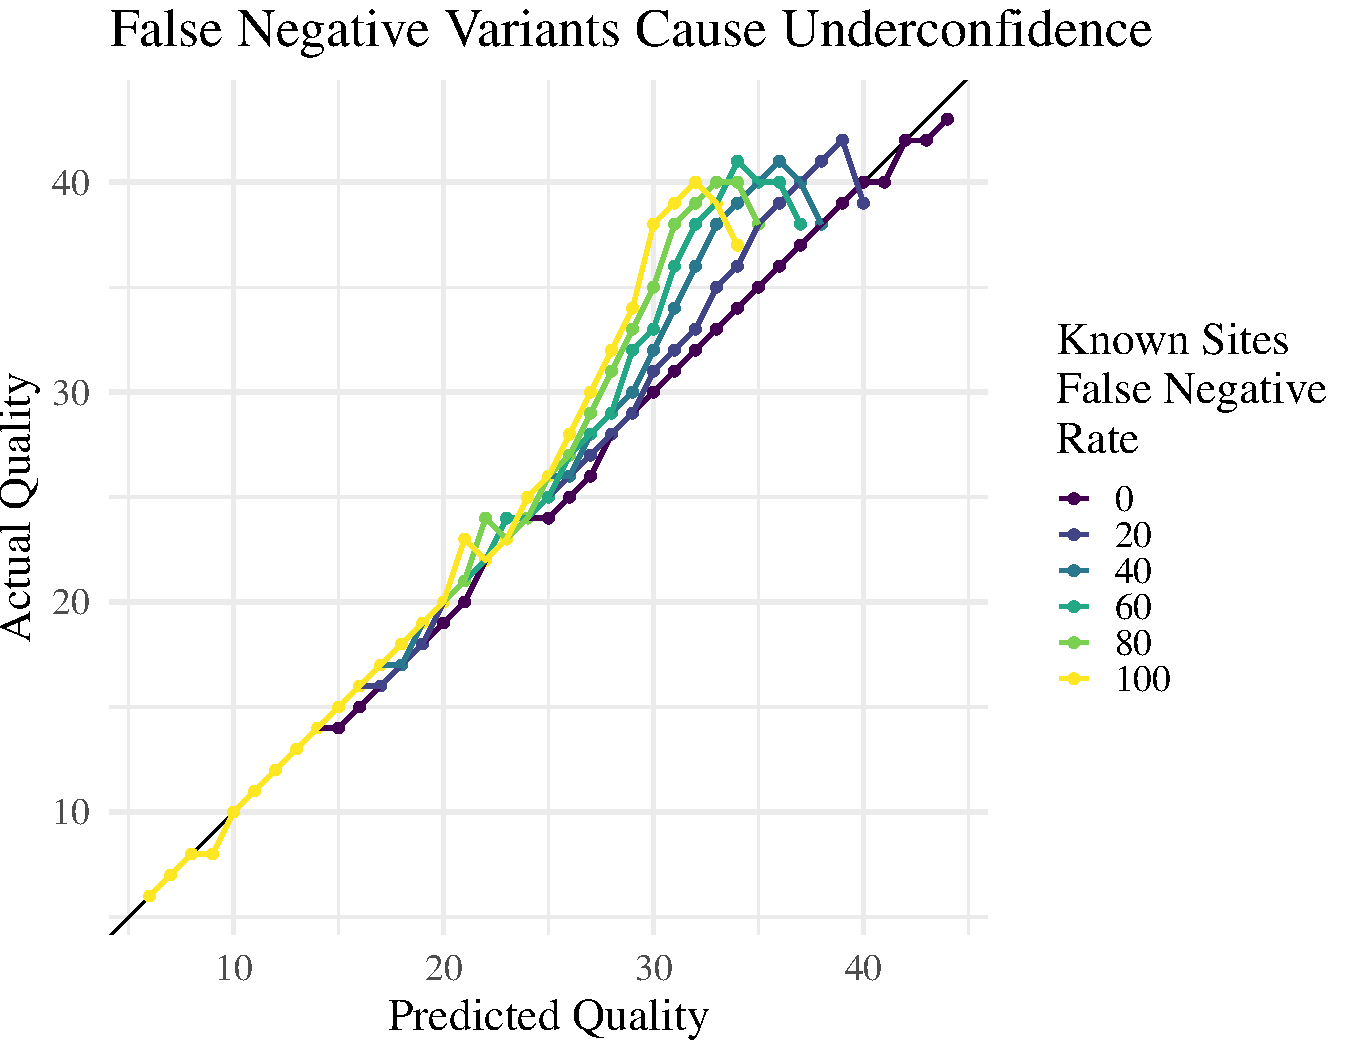
\includegraphics[width=.6\textwidth]{fnr.pdf}
	\titlecaption{False Negative Only Calibration}{Base quality score calibration for a range of false negatives in the database of variable sites. The false positive rate for all datasets is zero. Increasing the false negative rate significantly decreases the quality of the calibration, causing increasing  underconfidence in quality scores as the false negative rate rises.}
	\label{figure:fnr}
\end{figure}

\begin{table}
\centering
\begin{tabular}{r l}
\toprule
False Negative Rate & RMSE \\
\midrule
0 & 0.60 \\
20 & 1.32 \\
40 & 2.10 \\
60 & 2.57 \\
80 & 2.90 \\
100 & 3.20 \\
\bottomrule
\end{tabular}
\titlecaption{False Negative Calibration Errors}{Root mean squared error of quality score for reads recalibrated with a database of variable sites simulated with the given false negative rate. The false positive rate for each dataset is 0\%.}
\label{table:fnr}
\end{table}

To see if there were any interactive effects of false positive rate and false negative rate, I also simulated datasets with varying false positive and false negative rates. The RMSE of the calibrated scores is reported in Table \ref{table:fnrfpr} and summarized in Figure \ref{figure:fnrfpr}. These datasets were simulated separately from the above datasets, so there are slight differences in the calibration of the resulting reads.
As before, the number of false negatives significantly impacted calibration quality. In contrast to the false positive only dataset with a 0\% false negative rate, increasing the false positive rate also increased the amount of error in the calibration. Thus, false positives in the database of variable sites seem to enhance miscalibration caused by false negatives.

\begin{figure}
	\centering
	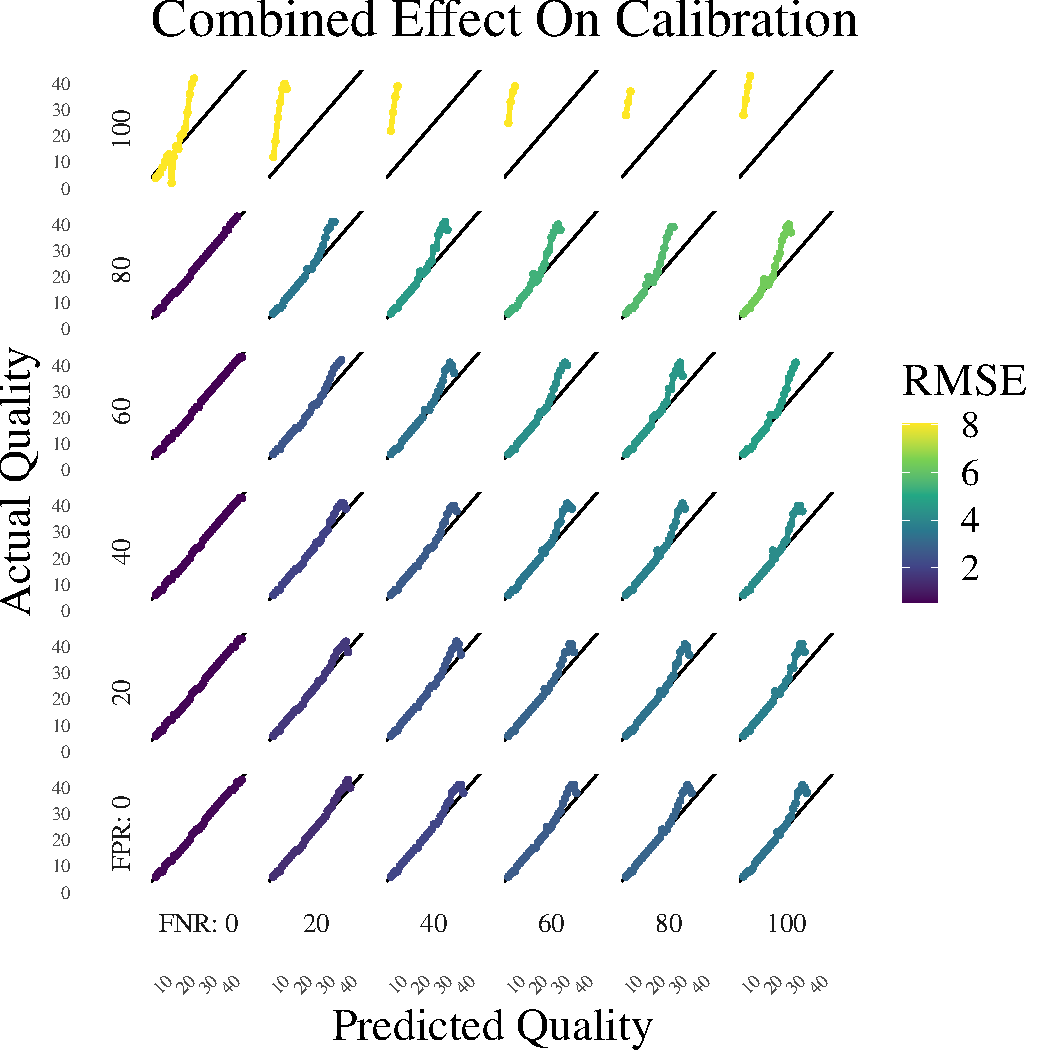
\includegraphics[width = \textwidth]{fnrfpr.pdf}
	\titlecaption{Combined Calibration}{Calibration of base quality scores of reads recalibrated using a database of variable sites with varying ranges of false negatives and false positives. The RMSE of the quality scores of the resulting calibration are used to color each line. Across the columns are each false negative rate, and each row represents a false positive rate. Except for at a false negative rate of 0, increasing either the false positive rate or the false negative rate increases the RMSE. See Table \ref{table:fnrfpr} for the RMSE values and the discussion in Section \ref{sec:kbbq_discussion} about false positive rates of 100\%}
	\label{figure:fnrfpr}
\end{figure}

\begin{figure}
	\centering
	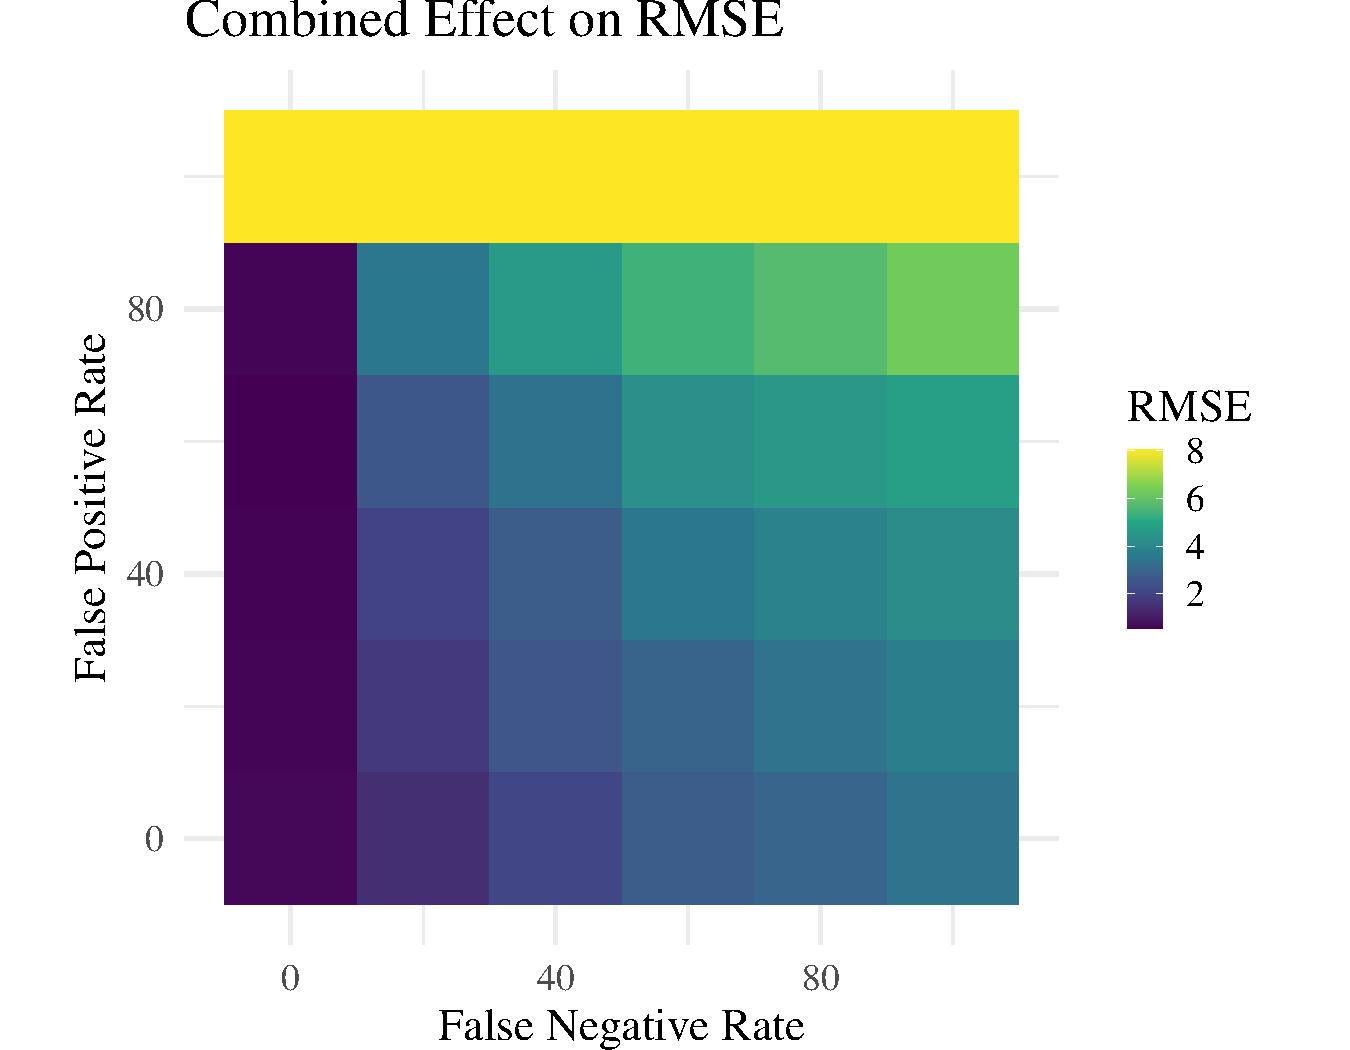
\includegraphics[width = .6\textwidth]{fnrfpr_heatmap.pdf}
	\titlecaption{Combined Calibration Heat Map}{Heat map of base quality calibration of varying ranges of false negatives and false positives. Databases of variable sites with differing false positive and false negative rates were constructed and the RMSE of the quality scores of the resulting calibration were calculated. Across the columns are each false negative rate, and each row represents a false positive rate. Except for at a false negative rate of 0, increasing either the false positive rate or the false negative rate increases the RMSE. See Table \ref{table:fnrfpr} for the RMSE values and the discussion in Section \ref{sec:kbbq_discussion} about false positive rates of 100\%}
	\label{figure:fnrfpr_heat}
\end{figure}

\begin{table}
\centering
\begin{tabularx}{.5\textwidth}{ l  X  X  X  X  X  X }
\toprule
\multirow{2}{*}{FPR} & \multicolumn{6}{c}{FNR} \\ \cmidrule(lr){2-7}
    & 0    &   20 &   40 &   60 &   80 &   100 \\
%&    &      &      &      &      &      & \\ %blank line
\midrule
0   & .641 & 1.45 & 2.08 & 2.73 & 2.99 & 3.38 \\
20  & .599 & 1.73 & 2.54 & 2.96 & 3.39 & 3.76 \\
40  & .555 & 2.02 & 2.71 & 3.50 & 3.84 & 4.16 \\
60  & .531 & 2.58 & 3.37 & 4.27 & 4.51 & 4.73 \\
80  & .593 & 3.52 & 4.62 & 5.38 & 5.73 & 6.32 \\
100 & 8.05 & 22.0 & 24.3 & 26.4 & 25.8 & 28.9 \\
\bottomrule
\end{tabularx}
\titlecaption{Combined Calibration Errors}{Root mean squared error of base quality score for data calibrated with databases of variable sites containing different levels of false positives and false negatives. The columns indicate false positive rates, the rows indicate false negative rates. The values in each cell are the RMSE of the quality scores for the reads recalibrated with the database of variable sites with false positive and false negative rate appropriate for its row and column. See Figure \ref{figure:fnrfpr_heat} for a graphical representation. The data in the 100\% false positive rows are likely artifacts; see section \ref{sec:kbbq_discussion} for more information.}
\label{table:fnrfpr}
\end{table}

Using GATK's recommended method of using high-confidence variants when a database of variable sites is unavailable produced poorly calibrated data with a RMSE of 3.89. This RMSE is similar to the RMSE of a simulated dataset with a false negative rate of approximately 60\%and a false positive rate around 40\%. However, the shape of this recalibrated data is also interesting; it shows that the quality scores are underconfident for mid-range quality scores and overconfident for high quality scores. This calibration and the calibration using the truth set, using KBBQ, and the raw read quality are plotted in Figure \ref{figure:comparison} and the RMSEs of each data set is listed in Table \ref{table:comparison}

\begin{figure}
\centering
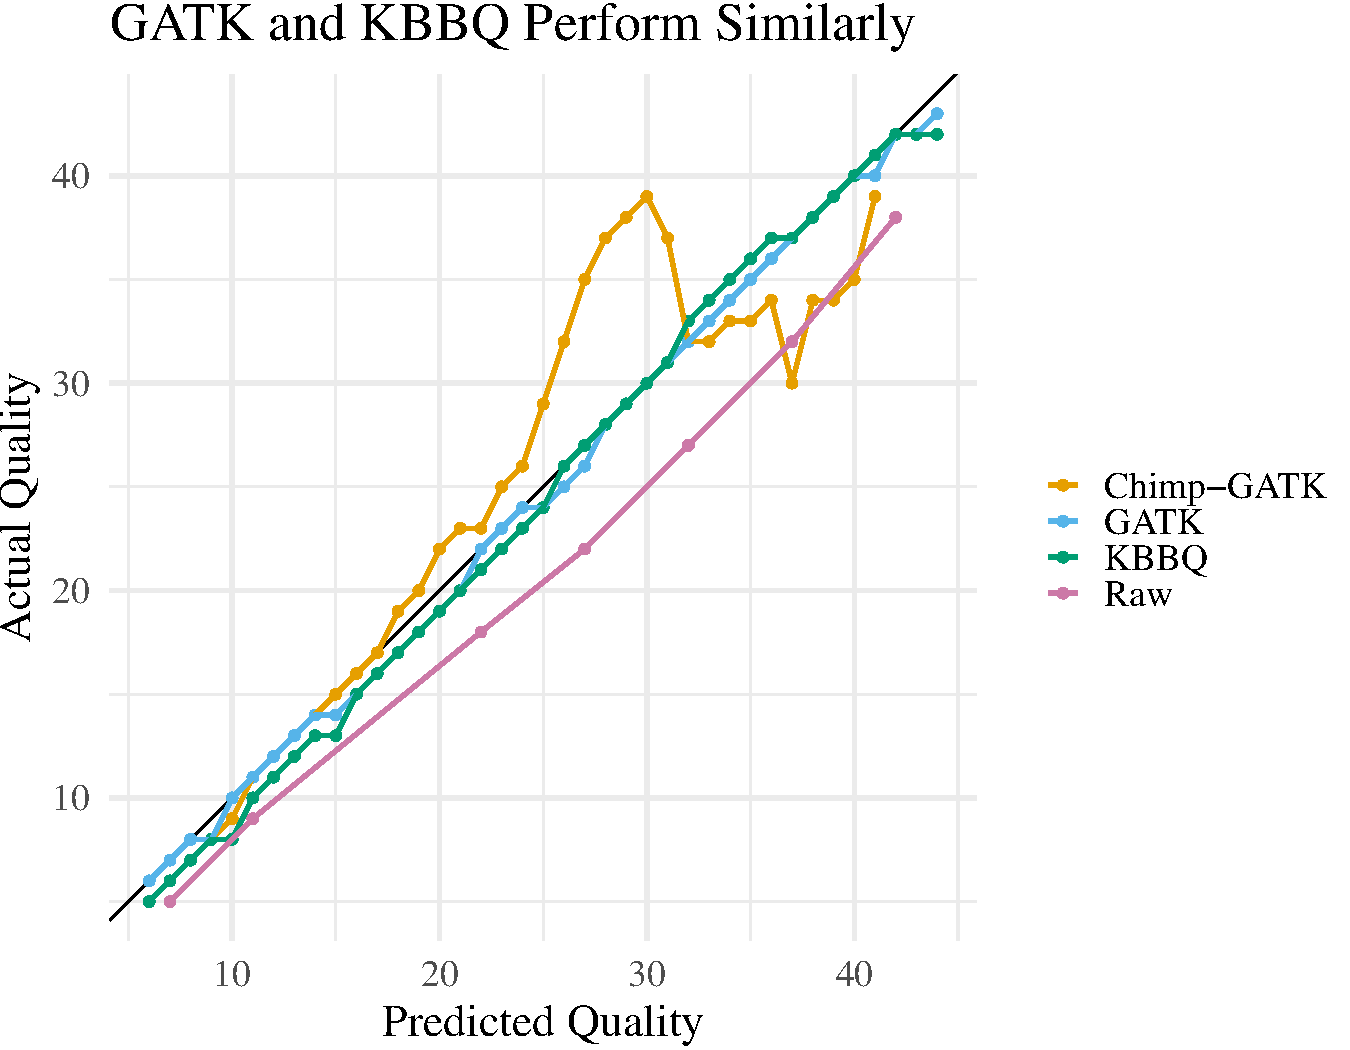
\includegraphics[width = .6\textwidth]{comparison.pdf}
\titlecaption{Comparison of Calibration Methods}{Chimp-GATK is the result of calibrating the reads using the model trained on the reads aligned to the chimp genome along with the variants called using that alignment. GATK is the result of using GATK's BaseRecalibrator with the truth set of variants. KBBQ is the result of using the KBBQ tool, which requires only reads and no reference or variant set. Raw is the calibration of the uncalibrated data.}
\label{figure:comparison}
\end{figure}

\begin{table}
\centering
\begin{tabular}{r l}
\toprule
Calibration Method & RMSE \\
\midrule
Chimp-GATK & 3.89 \\
GATK & 0.60 \\
KBBQ & 0.96 \\
Raw & 4.05 \\
\bottomrule
\end{tabular}
\titlecaption{Errors of Different Calibration Methods}{Root mean squared error of quality score for reads recalibrated using different methods. Chimp-GATK is the result of calibrating the reads using the model trained on the reads aligned to the chimp genome along with the variants called using that alignment. GATK is the result of using GATK's BaseRecalibrator with the truth set of variants. KBBQ is the result of using the KBBQ tool, which requires only reads and no reference or variant set. Raw is the calibration of the uncalibrated data.}
\label{table:comparison}
\end{table}

The resulting calibration of each recalibration method applied to the simulated data is shown in Figure \ref{fig:sim_comparison}. The raw data as simulated is fairly well-calibrated and almost all quality scores are on the 1-to-1 line. GATK recalibration with an initial callset caused calibration errors in high scoring bases. GATK recalibration caused a large calibration error for bases assigned a score of 20, which contained very few errors. However, there were also relatively few bases assigned a score of 20, as seen in Figure \ref{fig:sim_qual_counts}. The errors are summarized in Table \ref{table:sim_comparison}; KBBQ has the lowest RMSE, while GATK calibration using an initial HaplotypeCaller callset has the highest RMSE.

\begin{figure}
\centering
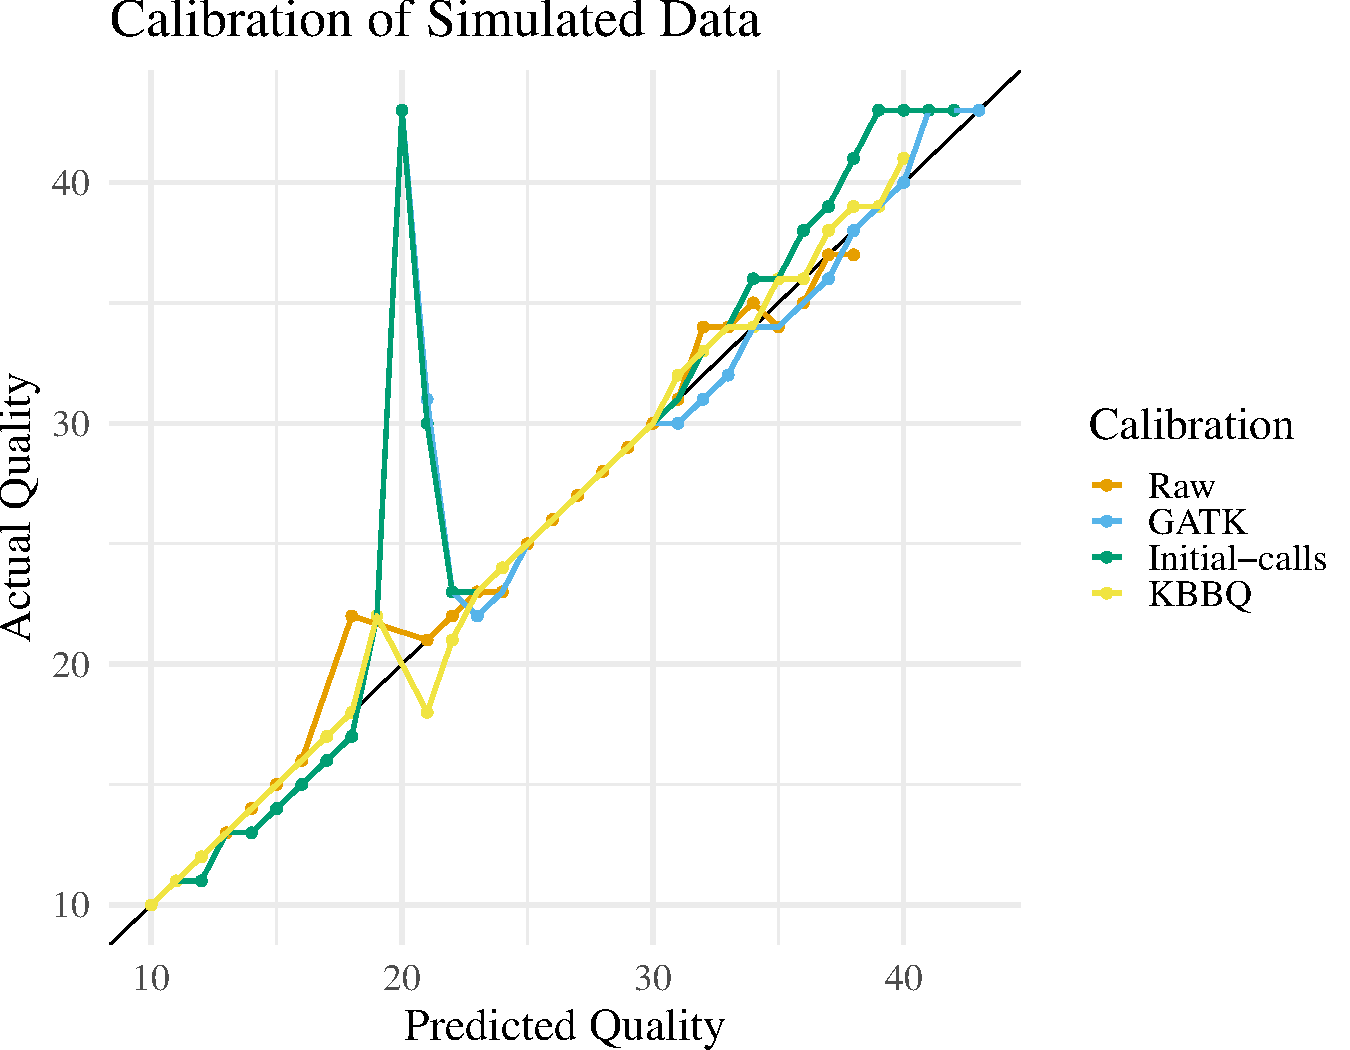
\includegraphics[width = .6\textwidth]{sim_comparison.pdf}
\titlecaption{Comparison of Calibration Methods on Simulated Data}{Plot of calibration errors before and after recalibrating reads simulated with ART. Raw is the unmodified simulated quality scores. GATK is the result of using BaseRecalibrator and ApplyBQSR using the set of true simulated variants as the known sites file. Initial-calls is the result of using BaseRecalibrator and ApplyBQSR but using an initial HaplotypeCaller callset rather than the true set of variants. KBBQ is the result of using KBBQ, a reference-free recalibration method. Note that the raw calibration lies almost all on the 1-to-1 line, meaning the data is already fairly well-calibrated.}
\label{fig:sim_comparison}
\end{figure}

\begin{figure}
\centering
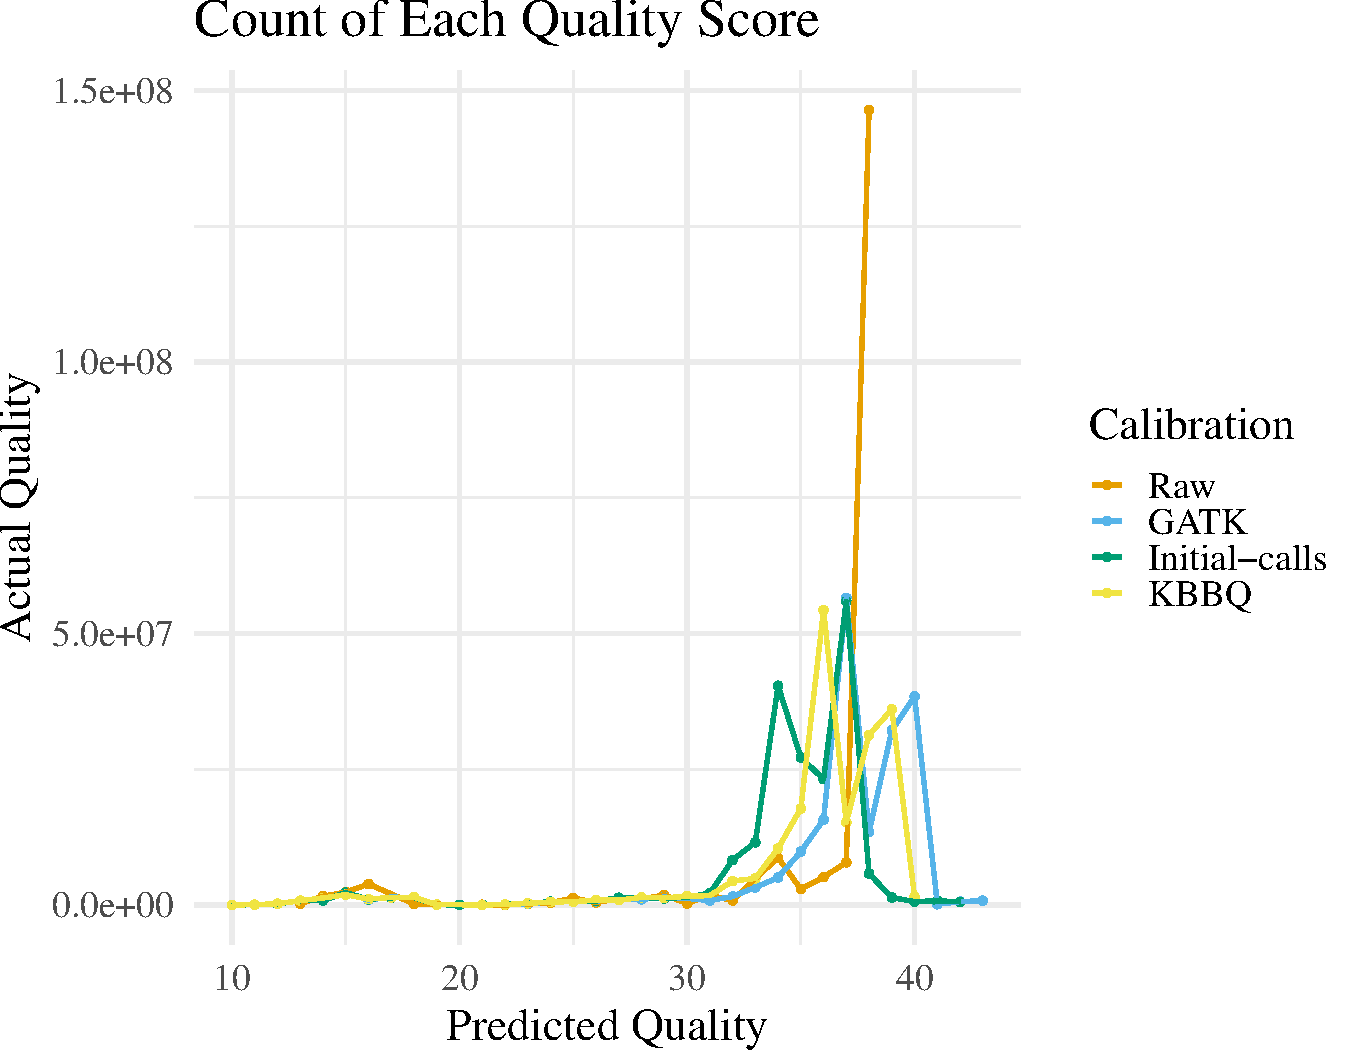
\includegraphics[width = .6\textwidth]{sim_qual_counts.pdf}
\titlecaption{Quality Score Distribution of Recalibrated Simulated Data}{Plot of the counts of each quality score in each dataset recalibrated by different methods. Raw is the unmodified simulated quality scores. GATK is the result of using BaseRecalibrator and ApplyBQSR using the set of true simulated variants as the known sites file. Initial-calls is the result of using BaseRecalibrator and ApplyBQSR but using an initial HaplotypeCaller callset rather than the true set of variants. KBBQ is the result of using KBBQ, a reference-free recalibration method. Most quality scores are above 30, and all the recalibration methods yield a distribution near that mode.}
\label{fig:sim_qual_counts}
\end{figure}

\begin{table}
\centering
\begin{tabular}{r l}
\toprule
Calibration Method & RMSE \\
\midrule
Raw & 1.06 \\
GATK & 4.40 \\
Initial-calls & 4.54 \\
KBBQ & 0.93 \\
\bottomrule
\end{tabular}
\titlecaption{Errors of Different Calibration Methods on Simulated Data}{Root mean squared error of quality score for simulated reads recalibrated using different methods. Raw is the unmodified simulated quality scores. GATK is the result of using BaseRecalibrator and ApplyBQSR using the set of true simulated variants as the known sites file. Initial-calls is the result of using BaseRecalibrator and ApplyBQSR but using an initial HaplotypeCaller callset rather than the true set of variants. KBBQ is the result of using KBBQ, a reference-free recalibration method. See Figure \ref{fig:sim_comparison} for a visualization of the calibration errors.}
\label{table:sim_comparison}
\end{table}

\section{Discussion}
\label{sec:kbbq_discussion}
These results show that GATK BaseRecalibrator is particularly vulnerable to false negatives (Figure \ref{figure:fnr}) in the database of variable sites, but is robust to false positives if the false negative rate is near 0 (Figure \ref{figure:fpr}). At the same time, when the false negative rate is not near 0, false positives will start to impact the calibration quality (Figure \ref{figure:fnrfpr}). Thus, when this database is unavailable and construction is required, it may be better to be liberal in deciding which sites may be variable to reduce the false negative rate as much as possible. This is in contrast to the GATK recommendation to use only the most confident sites when a database is unavailable.

The only rate that shows significant deviation from a 0\% false positive rate in the false-positive-only data is the 100\% false positive rate. Though a 100\% false positive rate with a 0\% false negative rate implies every site should be considered variable and ignored, the model curiously still has a source of errors it uses to recalibrate. Upon further investigation, this effect is driven by reads with alignments that begin with an insertion, as these inserted bases are not ignored by BaseRecalibrator when the first position of the site that should be ignored is equal to the first aligned position in the read. Thus, this line is a technical artifact. So long as there are enough bases available to analyze, the false positive rate doesn't significantly affect the performace of BaseRecalibrator at a false negative rate of 0. The calibrations of other datasets with a false positive rate of 100\% would also be affected by this artifact; however, in a real dataset it's unlikely to ever achieve a false positive rate of 100\%, so this artifact is unlikely to significantly affect real data.

%new para
Ultimately, if the false negative and false positive rates of the database of variable sites is high, GATK's procedure for BQSR \textit{can} cause miscalibration of the data worse than using raw quality scores, though this can only happen with very large error rates. In this dataset, the raw data has a RMSE of about 4, which is similar to a simulated dataset with a false negative rate between 40-60\% and a false positive rate between 60-80\%. In a real situation it's unlikely that error rates like this will occur, so BQSR will not severely destroy the input data. However, at even modest false negative and false positive error rates BQSR can cause undesirable miscalibration that could feasibly impact variants called from the data. Interestingly, at all error rates the calibration of quality scores below 25 is almost always correct or 1-off the true value. It seems that errors in the database of variable sites have a larger effect on higher quality predictions than lower ones.

At the same time, the calibration model trained with the chimp-aligned data shows performance worse than a simulated dataset with a false negative rate around 40-60\%. The RMSE of 3.89 is only slightly better than the RMSE of the raw data and the plotted calibration shows very poor performance at higher quality scores. Additionally, quality scores assigned between 25 and 32 were significantly different than the true quality scores. And while all the simulated datasets caused underconfidence in the calibration, this calibration method caused overconfidence in quality scores above 34.

This suggests that an effect not captured in the simulated data was present in this data. Overconfidence indicates errors that should be counted by the model are instead missed and therefore there are more errors in actuality than the model predicts. Thus the set of variants used to skip errors is too aggressive and contains many false positives. So why is a similar effect not observed in the simulated data? This is likely because of how the simulated datasets were constructed; non-variable sites were selected independently and at random to be added to the set of purported variable sites. Thus a site containing an error and a site not containing an error are selected proportionally. In contrast, on a real dataset a variant calling algorithm would not make false positive errors independently; it is much more likely to classify a site as variable that has a sequencing error than to classify a site as variable that has no errors. That is: in this simulation, $P(\operatorname{classified\:positive} | \operatorname{actual\:negative})$ is independent of $P(\operatorname{sequencing\:error})$, but on an empirical dataset $P(\operatorname{classified\:positive} | \operatorname{actual\:negative})$ is likely not. Thus in reality false positives probably cause overconfidence in a similar manner that false negatives cause underconfidence. This overconfidence is observed in the Chimp-GATK calibration method.

As the chimp-aligned calibration shows, GATK BQSR struggles on real data from non-model organisms. False negatives are likely to be numerous in almost all but the most well-studied samples \parencite{bobo_false_2016}, and false positives are similarly likely when using poor quality, draft reference genomes that cause alignment errors. This means in most datasets, while its performance may be acceptable if the false negative and false positive rate are sufficiently low, GATK BaseRecalibrator is not the best recalibration method. This is shown in Figure \ref{figure:comparison}, which shows \texttt{kbbq} performing nearly as well as GATK BQSR with perfect knowledge of variable sites. However, \texttt{kbbq} doesn't use any reference or any variant site information to do recalibration. \texttt{kbbq} also performs much better than GATK's recommended procedure when a database of variable sites is not available, as shown in the Chimp-GATK calibration.

Recalibration of the simulated reads shows that KBBQ is able to recalibrate reads even if they are already well-calibrated without severely damaging the calibration of the quality scores. In contrast, using GATK even with an accurate database of variable sites introduces additional error in quality score calibration to the reads, with both GATK-based methods having much higher RMSE than the raw quality scores. Additionally, even though the reads were already fairly well-calibrated, KBBQ recalibration confers a slight improvement to the RMSE of the quality scores. All methods yielded quality scores near 38, the mode of the raw quality data.

% While there is a large spike in calibration error for bases assigned a score of 20, most of the data is assigned a score around 38, which is the mode of the raw data. This spike is a large contributor to the RMSE, but doesn't represent a very significant difference to the overall quality of the calibration. However, miscalibration in bases with quality scores between 32 and 40 are likely very important for the overall quality of the calibration, since most bases are assigned scores in that range. In this range, all calibration methods except GATK using intial variant calls were fairly close.


\section{Conclusion}

Base quality score recalibration is an important procedure to ensure base quality scores are accurate before variant calling. However, the most popular method for doing BQSR is not easy to do if the sequenced organism is a non-model organism. I developed the software tool \texttt{kbbq} to recalibrate base quality scores without a reference or database of variable sites to overcome these deficiencies. Since it doesn't use a database of variable sites or a reference, the quality of these resources is immaterial to the quality of the resulting calibration.

To evaluate KBBQ, I emulated GATK's procedure for calibration when a database of variable sites is unavailable by aligning a synthetic diploid human benchmarking dataset to the chimp genome and calling variants to use as the database of variable sites. This method produces a calibration worse than \texttt{kbbq}. I further simulated reads from a draft assembly to simulate sequencing of a highly heterozygous non-model organism. Though the simulated data was fairly well-calibrated, GATK calibration with perfect knowledge of the heterozygous sites and using an initial set of calls introduced more error into the quality score calibration than was in the original data while KBBQ recalibration slightly reduced it. Thus, when a database of variable sites or reference is unavailable or of poor quality, \texttt{kbbq} is an effective method for base quality score recalibration.

%hapdip stuff that needs to be moved to ch5
I simulated sets of variable sites with varying false positive and false negative rates to use with BQSR. While it seems the simulated false positives are somewhat different from those that appear in real datasets, it is clear that false negatives severely reduce the quality of the calibration using GATK's method.

\printbibliography[segment=\therefsegment]{}

	% \item Future work: see how big the difference is in variant calls using binned quality scores, miscalibrated reads, and well calibrated reads.

\chapter{Evaluating the impact of quality score calibration on variant calling}
\label{ch:evaluating}
\section{Introduction}

DNA sequencing is a powerful tool applied in many fields of biology. Understanding how DNA and changes in DNA influence organisms and how they interact with their environment is a fundamental goal of genetics. Correctly identifying the composition of a sampled DNA molecule is therefore an important first step for many genetic studies. However, this task is not trivial; sequencing technology is inherently prone to errors which can make it difficult to discern true biological effects from technical errors \parencite{fox_accuracy_2014, wu_estimating_2017}. 

Because of this error, the same piece of DNA is usually sequenced multiple times to attempt to get multiple measurements and a model is applied to infer the sample genotype \parencite{li_statistical_2011, garrison_haplotype-based_2012, poplin_scaling_2018}. While a few sequencing errors do not impede accurate inference of the genotype of a monoploid sample, sequencing errors can be difficult to distinguish from heterozygosity in diploid organisms. This problem is even more difficult for samples with higher ploidy. However, using a statistical model enables a systematic approach to genotyping every site in the genome.

Additionally, a model allows the incorporation of auxiliary information when deciding the genotype at a site in a sample. For example, variant calling models often incorporate population genetic parameters that can help distinguish between sequencing errors and biological variation. The expected heterozygosity parameter \theta is particularly important; it usually paramaterizes some prior on the probability of a base matching the reference genome. If this deviates significantly from the true value, the model may mistakenly classify truly heterozygous sites as errors or vice versa.

The goal of using a model to call variants is to integrate a wide variety of information to make a principled decision about whether or not a variant exists. An important source of information on the trustworthiness of each sequenced base is the base quality score \parencite{ewing_base-calling_1998, ewing_base-calling_1998-1}. This is a score, usually between 2 and 43, that encodes the probability the sequence is an error in the Phred scale. That is, the score $Q = -10\log_{10}P(\operatorname{Base is an error})$. This number is then rounded to the nearest integer and encoded as a character, shifted by 33, in the sequencing data.

Since these numbers can vary significantly in the same line with few patterns, quality scores can't usually be compressed very well by common compression algorithms. That gives sequencing data large file sizes that make it expensive to store the data for a lengthy period of time. Thus, these quality scores are often binned to reduce the amount of variation in the scores, enabling improved compression \parencite{shibuya_better_2019, malysa_qvz_2015, yu_quality_2015, noauthor_reducing_2014}. Most binning methods attempt to do so in a way that minimizes the difference between the error rate of the bin and the error rate the bin should have according to its assigned score. However, there can still be a disconnect between the predicted error rate and the actual error rate. Furthermore, as the resolution of quality scores is reduced, some information about the true score at each base is lost. Interestingly, \cite{yu_quality_2015} find that compressing scores by removing quality scores from all sites that are not likely to vary based on the k-mer composition of the data, but keeping quality scores intact at sites that may contain errors or true variants increases the quality of output genotype calls.

To restore quality score resolution before analysis and to ensure quality scores accurately reflect the probability of error at every base, a process known as base quality score recalibration (BQSR) is sometimes performed \parencite{auwera_fastq_2013, pfeifer_next-generation_2017}. This attempts to use known information about sequencing errors to calibrate the quality scores. The most common method for doing so implemented in the Genome Analysis Toolkit (GATK) requires aligned reads and a set of variable sites that are removed from analysis. The algorithm then looks for bases that do not match the reference, assumes they are errors, and uses those errors to recalibrate the quality scores. See Chapter \ref{ch:kbbq} for more information on quality scores and base quality score recalibration.
	
The ultimate goal of quality scores and base quality score recalibration is to make it easier to identify erroneous bases, which should improve the set of variants a variant caller emits. However, evidence supporting the use of base quality score recalibration is limited and whether base quality score recalibration is worthwhile is subject to debate. The procedure has aided in detecting rare variants \parencite{ni_improvement_2016}, and a recalibration procedure that integrates mapping errors into quality scores seems to improve variant detection \parencite{li_improving_2011}. The goal of this chapter is to investigate the degree that base quality score recalibration affects variant calling to enable informed decisions for constructing variant calling pipelines, especially for non-model organisms.

\section{Methods}

% Subsampling of database of variable sites - move this to Ch5
In order to determine how misspecification of the database of variable sites affects the calibration of GATK's BQSR procedure \parencite{auwera_fastq_2013}, I simulated datasets with various levels of false negative and false positive variants. In this case, false negative variants in the database of variable sites causes a site that should be ignored to not be ignored, greatly increasing the number of bases that GATK classifies as sequencing errors. On the other hand, false positive variants remove a site from GATK classification, so the effect is likely to be small except for large false positive rates.

To create each simulated dataset, I began with the high coverage synthetic diploid dataset described in \cite{li_synthetic-diploid_2018} with reads aligned to hg19. This dataset was constructed by mixing DNA from the CHM1 and CHM13 hydatidiform mole cell lines to create a synthetic diploid sample. It inclued a VCF of variant calls and a BED file representing regions where the authors are confident the calls in the VCF are correct.

To create each false negative dataset, an appropriate number of sites from the VCF were randomly sampled with BCFTools and the shuf program. To create each false positive dataset, all sites from the VCF were extracted in BED format with the BCFTools query command, then subtracted from the BED of confident regions with bedtools subtract \parencite{quinlan_bedtools_2010}. The appropriate number of sites were then sampled with the shuf program and appended to the sites from the VCF to generate the BED file of all sites to exclude. Thus, I created variable site sets that were artificially crafted to have different rates of false positive and false negative calls, from 0 to 100 in steps of 20.
These files were then provided as input to GATK's BaseRecalibrator tool and calibration was evaluated with GATK's AnalyzeCovariates tool.

As a control, I compared each result to the raw, uncalibrated data. To see how a reference-free recalibration method affected variant calling, I also recalibrated the data with \texttt{kbbq}, with the options -\phantom{}-genomesize 214206308 and -a .15 .

I then called variants on each dataset using GATK HaplotypeCaller \parencite{poplin_scaling_2018}. The false positive rate of 100\% produced no output calls except in the case of 0\% false negative rate, which produced fewer calls than any other set. All datasets containing a 100\% false positive rate were therefore discarded. I evaluated these output SNP calls using RealTimeGenomics' RTG Tools vcfeval program \parencite{cleary_comparing_2015} and the the confident region set along with the confident call set. I first ran the tool using the default settings, which also produces a ROC curve for the calls' GQ annotation. I also ran the tool using the -\phantom{}-vcf-score-field=QUAL option, which produces ROC curves for the site's QUAL annotation. This enabled comparison of the sensitivity and false positive rate trade-off of the two scores for each dataset. These two annotations were chosen because they represent an overall summary of the quality of the called variants.

The false positive rate for the ROC curves was found by dividing the number of false positive calls in each dataset at each value of QUAL or GC and below by the number of true negative sites. The number of true negative sites was obtained by subtracting each true positive variant from the BED file containing the confident regions of the callset. This rate had to be computed, as vcfeval does not report a false positive rate. As the RTG-tools manual states, the program doesn't try to compute the possible number of true negatives, as calls could in theory occupy many or no reference bases. However, as I analyze only SNP data here,  estimating the true number of negatives as the number of sites that are within the confident regions but outside variant sites specified by the truth set should be sufficient. The true positive rate was calculated by taking the number of true positive calls in each dataset for each value of QUAL or GC and dividing by the number of positive calls in the truth set, as reported by the vcfeval output.

To evaluate the output calls, I plotted the number of false positive and true positive SNP calls for each dataset. I also constructed a heat map showing the F-statistic of each dataset. This is the harmonic mean of the sensitivity and precision of the calls and is one way to summarize the accuracy of the calls. All plots and heatmaps were made using R \parencite{r_core_2020} and ggplot2 \parencite{wickham_ggplot2_2016} using the viridis color pallete \parencite{garnier_viridis_2018} to ensure the plots remain interpretable by those with colorblindness and after photocopying.

%Filter info + justifications:
%#filter: only snps
%#filter: DP > 35 & DP < 65 (+-2 SDEV from mean of ~50 assuming poisson)
%#filter: QUAL > 75; this is ~bottom 1% and the maximum F
%#   value from the previous analysis is between 75 and 150.
To see how filtering the calls affected their quality, I then identically filtered each variant set with two filters using bcftools view \parencite{li_sequence_2009}. The first filter is a depth filter, only accepting variants that have more than 35 aligned reads and fewer than 65. This is within two standard deviations of the mean sequencing depth of \~50, assuming the read depths are Poisson distributed. The second filter is a QUAL filter, accepting only calls with a QUAL of over 75. This threshold was chosen because it is approximately the bottom 1\% of QUAL values in each dataset and it is the lowest QUAL value that maximizes the F-statistic of all the datasets. I then calculated the same statistics and made the same plots using the filtered calls.

%THE STORY IS COMING TOGETHER: The range in number of TP calls grows after filtering! Prior to filtering there is a big difference in the number of FPs in each dataset (1009), but this difference shrinks after filtering to 548. The difference in number of true positives starts at 240, but grows to 2044 after filtering.


%Simulated reads
%
In order to investigate how calibration affected variant calling performance on a medium-coverage dataset from a highly heterozygous sample with a low-quality reference, as might be the case when sequencing a non-model organism, I created a simulated dataset. I first randomly sampled contigs from the first release of the \textit{Eucalyptus grandis} reference (SRA accession ) until I sampled 5 million base-pairs, which at 20X coverage for a diploid genome would yeild approximately 200 million base-pairs of synthetic sequence data. I then simulated heterozygous sites in the genome with simuG \parencite{yue_simug_2019} with a transition/transversion ratio of 2 and 125,000 SNPs to emulate the conditions observed in eucalypts \parencite{kulheim_comparative_2009}. I concatenated the subsampled and simulated genomes to create a diploid reference and simulated reads from it using ART \parencite{huang_art_2012}. I simulated 101-bp long reads with a mean fragment length of 300 and standard deviation of 20, with 20X coverage. I then aligned the simulated reads to the genome with NextGenMap \parencite{sedlazeck_nextgenmap_2013} and recalibrated the data 3 ways: 1) with GATK using the true set of heterozygous sites as the database of variable sites, 2) with GATK using a set of variant calls generated with HaplotypeCaller with the \texttt{-\phantom{}-stand-call-conf} set to 50 as the database of variable sites, and 3) using KBBQ (see Chapter \ref{ch:kbbq}) with the genome size parameter set to 5 million.

Including the simulator-assigned raw scores, this yielded four datasets with different quality scores to call variants with and compare the results. HaplotypeCaller was used on each dataset and given the subsampled genome as a reference and called with the \texttt{-\phantom{}-heterozygosity 0.025} option to represent the approximate heterozygosity of the data. As simuG doesn't output sample genotypes and the simulated sample is heterozygous at every site in the truth VCF, a sample column was added and the genotype of the sample at every site set to be 0|1 using sed. This VCF was then used as the truth comparison for rtg-tools vcfeval command and used to evaluate each set of variant calls. vcfeval was run in annotate mode and the output parsed using hapdip.js to generate summaries of each callset. Finally, vcfeval was also run in roc-only mode, once with the --vcf-score-field set to GQ and once set to QUAL to produce ROC curves for each of these scores. The false negative rate was obtained by dividing the number of output false negatives by the length of the genome minus the number of simulated heterozygous sites.

% /storage/2017-03-15-eucalyptus/2020-09-28-kbbqflt
Finally, I ran KBBQ with the specified genome size 605951511 and coverage 240 to recalibrate a set of reads sequenced from an individual of the non-model species \textit{Eucalyptus melliodora} \parencite{orr_phylogenomic_2020}. This dataset contains reads from 3 leaves each from 8 branches, each leaf sequenced to a depth of approximately 10X. I then called variants using HaplotypeCaller and filtered the calls using the same filters from \cite{orr_phylogenomic_2020}. At each filtering step, I took the approach described in Appendix \ref{ch:structured} to estimate the false discovery rate and false negative rate. Briefly, I created 100 random trees that were maximally distant from the true tree structure and filtered using these random trees instead of the true tree. Any variants that appeared in any of the randomized trees but not in the set of variants identified in \cite{orr_phylogenomic_2020}, I classified as false positives. To estimate the false negative rate, I counted the number of variants in the previously identified calls that were not found via HaplotypeCaller. I then compared these values to those found using the raw, uncalibrated reads and those found using GATK recalibrated reads in \cite{orr_phylogenomic_2020}.

Scripts to reproduce these analyses are included in Appendix \ref{ch:evaluating_code}.

\section{Results}
% Hapdip Analysis
To identify how errors in the database of variable sites affects variant calling, I simulated different datasets with known false positive rates, plotted the calibration and calculated the root mean squared error (RMSE) of the data recalibrated with the model trained using each database as the known sites input to GATK BaseRecalibrator. These plots are shown in figure \ref{figure:fpr}, and the RMSE of the quality score for each dataset is shown in table \ref{table:fpr}. For all these datasets, the false negative rate is 0. As the false positive rate increases, the degree of miscalibration doesn't change significantly except for the 100\% false positive rate dataset, which is very poorly calibrated; however, this calibration is likely an artifact (see section \ref{sec:kbbq_discussion}).

\begin{figure}
\centering
	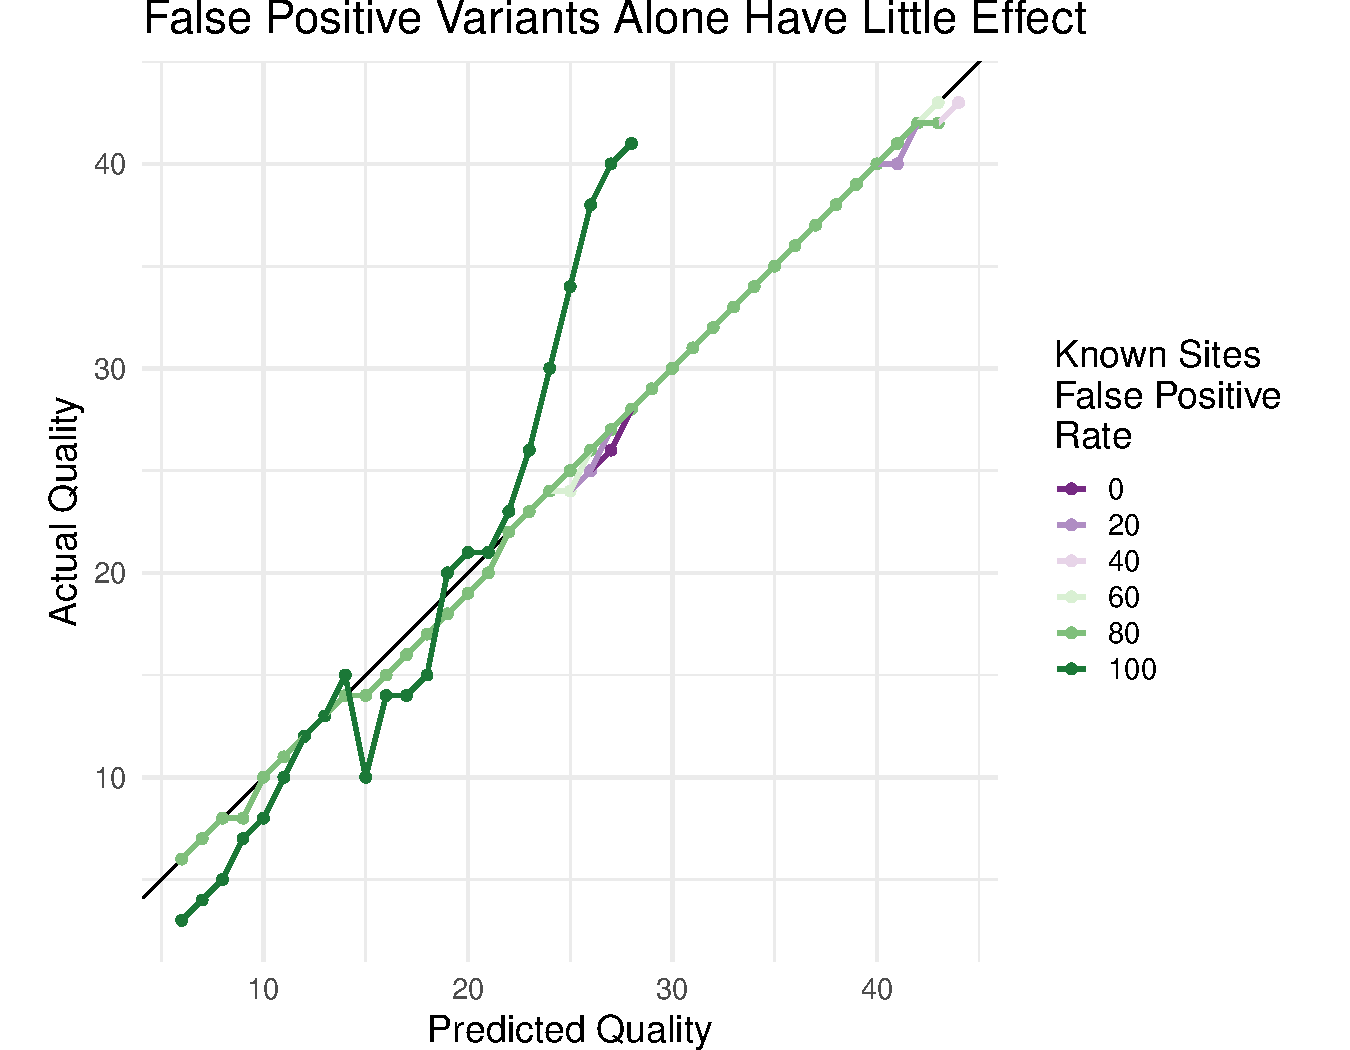
\includegraphics[width = .6\textwidth]{fpr.pdf}
	\titlecaption{False Positive Only Calibration}{Base quality score calibration for a range of false positives in the database of variable sites. The false negative rate for all datasets is zero. Increasing the false positive rate does not significantly impact the quality of the calibration. The poor calibration at a 100\% false negative rate is likely an artifact (see Section \ref{sec:kbbq_discussion}).}
	\label{figure:fpr}
\end{figure}

\begin{table}
\centering
\begin{tabular}{r l}
\toprule
False Positive Rate & RMSE \\
\midrule
0 & 0.60 \\
20 & 0.58 \\
40 & 0.53 \\
60 & 0.49 \\
80 & 0.49 \\
100 & 5.50 \\
\bottomrule
\end{tabular}
\titlecaption{False Positive Calibration Errors}{The root mean squared error of quality score for reads recalibrated using a database of variable sites with different false positive rates. The false negative rate for each dataset is 0\%.}
\label{table:fpr}
\end{table}

I also simulated different databases of variable sites with differing false negative rates and similarly used it to recalibrate the CHM1-CHM13 data. In these datasets, the false positive rate is 0\%. The plotted calibration and RMSE of the recalibrated data is shown in figure \ref{figure:fnr} and table \ref{table:fnr}. As the false negative rate increases, the degree of miscalibration also steadily increases.

\begin{figure}
	\centering
	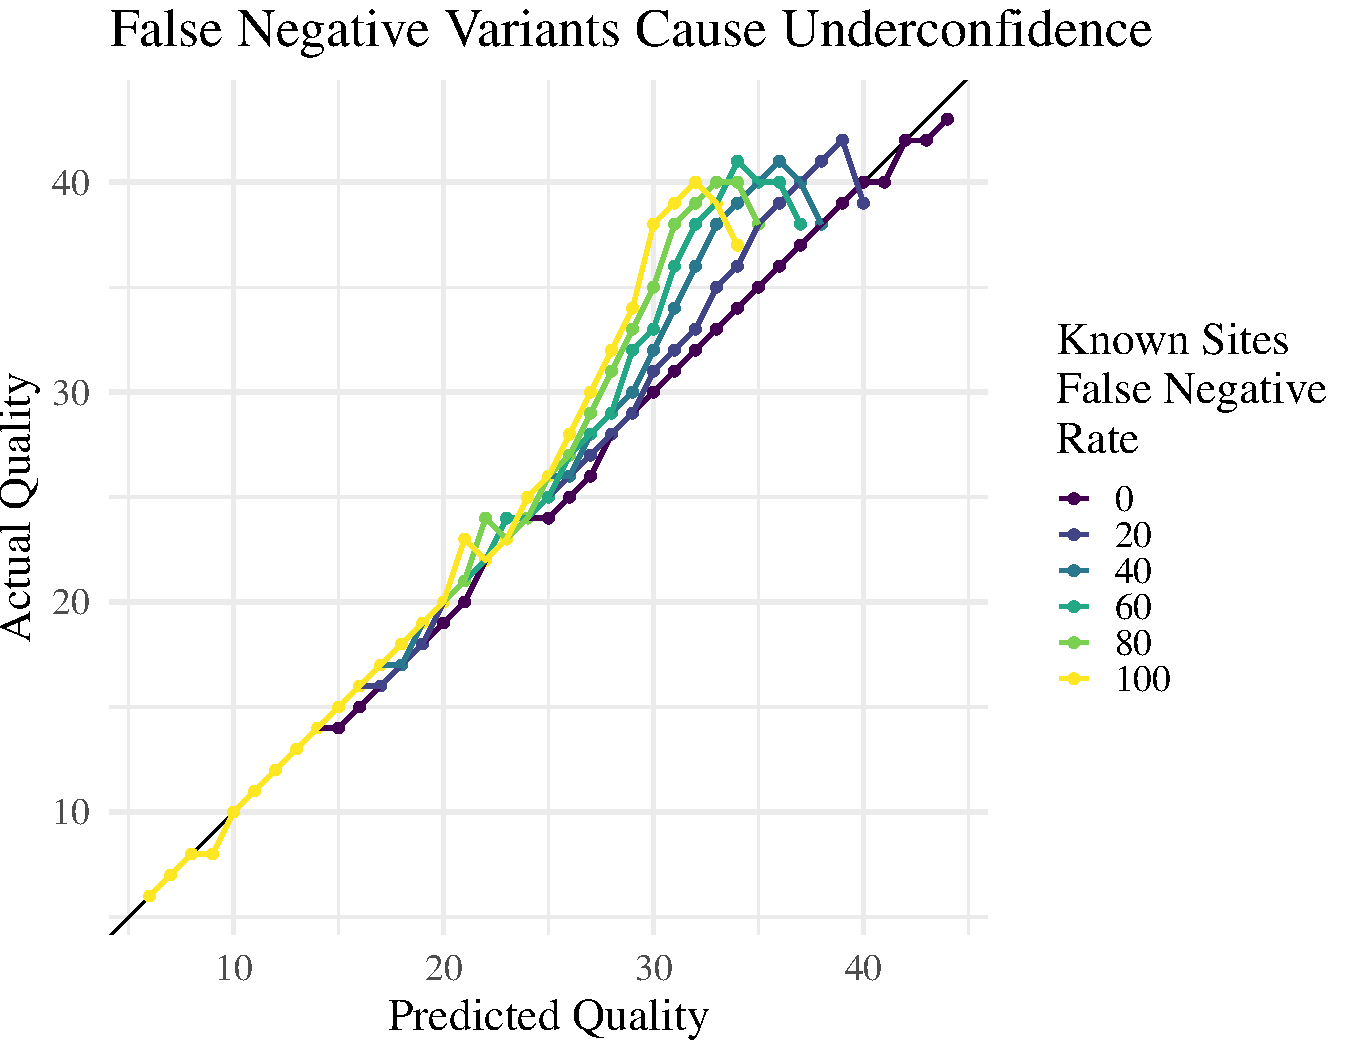
\includegraphics[width=.6\textwidth]{fnr.pdf}
	\titlecaption{False Negative Only Calibration}{Base quality score calibration for a range of false negatives in the database of variable sites. The false positive rate for all datasets is zero. Increasing the false negative rate significantly decreases the quality of the calibration, causing increasing  underconfidence in quality scores as the false negative rate rises.}
	\label{figure:fnr}
\end{figure}

\begin{table}
\centering
\begin{tabular}{r l}
\toprule
False Negative Rate & RMSE \\
\midrule
0 & 0.60 \\
20 & 1.32 \\
40 & 2.10 \\
60 & 2.57 \\
80 & 2.90 \\
100 & 3.20 \\
\bottomrule
\end{tabular}
\titlecaption{False Negative Calibration Errors}{Root mean squared error of quality score for reads recalibrated with a database of variable sites simulated with the given false negative rate. The false positive rate for each dataset is 0\%.}
\label{table:fnr}
\end{table}

To see if there were any interactive effects of false positive rate and false negative rate, I also simulated datasets with varying false positive and false negative rates. The RMSE of the calibrated scores is reported in Table \ref{table:fnrfpr} and summarized in Figure \ref{figure:fnrfpr}. These datasets were simulated separately from the above datasets, so there are slight differences in the calibration of the resulting reads.
As before, the number of false negatives significantly impacted calibration quality. In contrast to the false positive only dataset with a 0\% false negative rate, increasing the false positive rate also increased the amount of error in the calibration. Thus, false positives in the database of variable sites seem to enhance miscalibration caused by false negatives.

\begin{figure}
	\centering
	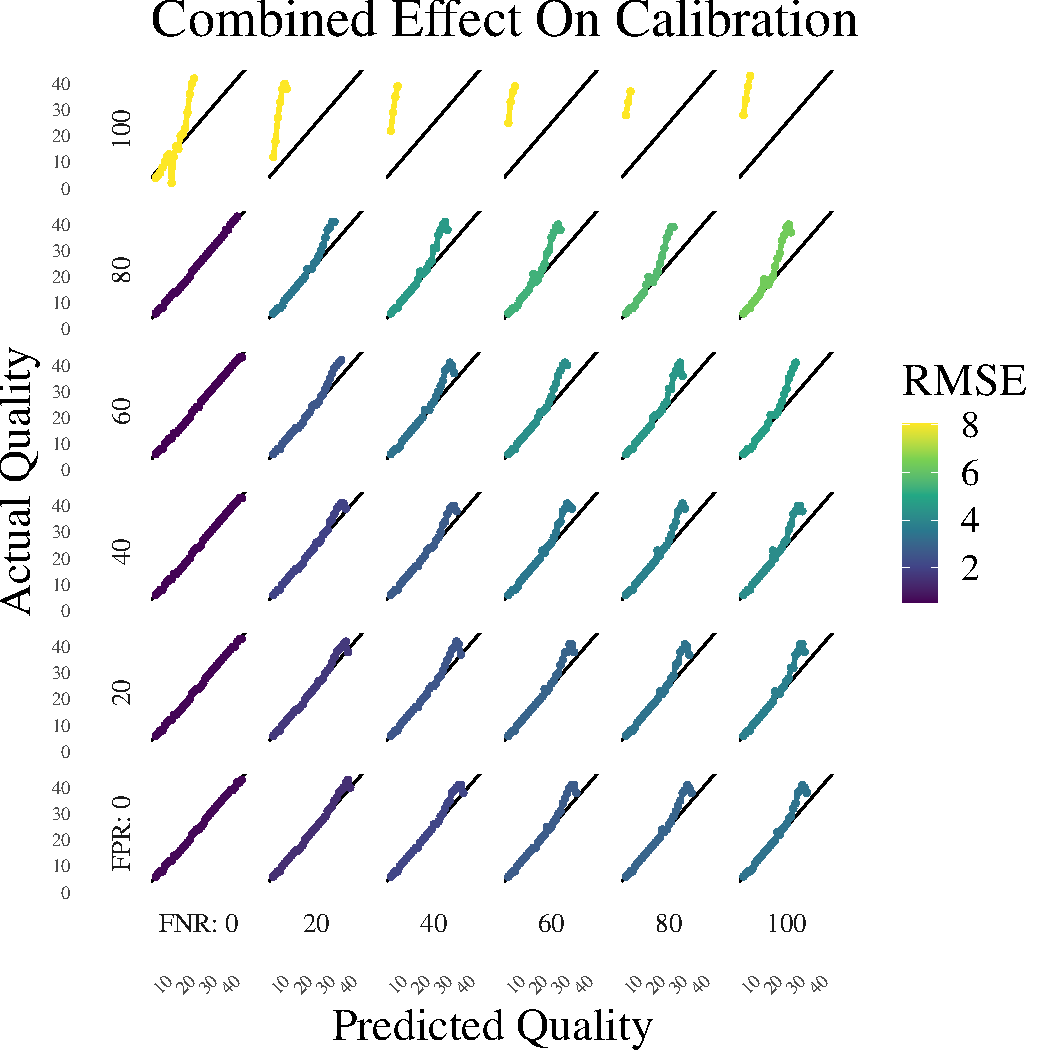
\includegraphics[width = \textwidth]{fnrfpr.pdf}
	\titlecaption{Combined Calibration}{Calibration of base quality scores of reads recalibrated using a database of variable sites with varying ranges of false negatives and false positives. The RMSE of the quality scores of the resulting calibration are used to color each line. Across the columns are each false negative rate, and each row represents a false positive rate. Except for at a false negative rate of 0, increasing either the false positive rate or the false negative rate increases the RMSE. See Table \ref{table:fnrfpr} for the RMSE values and the discussion in Section \ref{sec:kbbq_discussion} about false positive rates of 100\%}
	\label{figure:fnrfpr}
\end{figure}

\begin{figure}
	\centering
	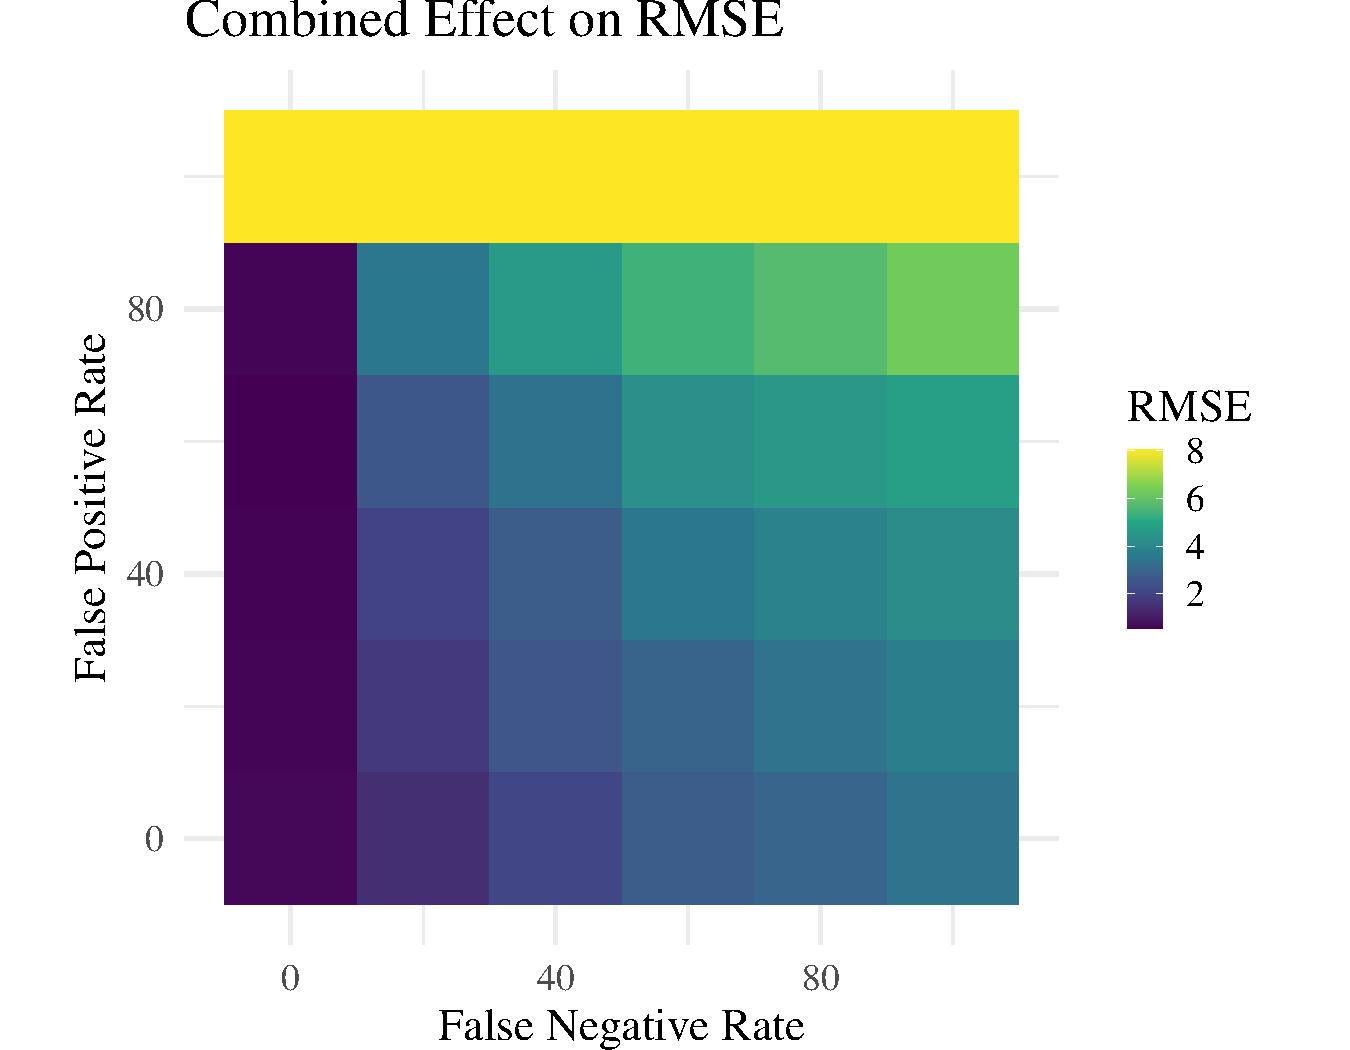
\includegraphics[width = .6\textwidth]{fnrfpr_heatmap.pdf}
	\titlecaption{Combined Calibration Heat Map}{Heat map of base quality calibration of varying ranges of false negatives and false positives. Databases of variable sites with differing false positive and false negative rates were constructed and the RMSE of the quality scores of the resulting calibration were calculated. Across the columns are each false negative rate, and each row represents a false positive rate. Except for at a false negative rate of 0, increasing either the false positive rate or the false negative rate increases the RMSE. See Table \ref{table:fnrfpr} for the RMSE values and the discussion in Section \ref{sec:kbbq_discussion} about false positive rates of 100\%}
	\label{figure:fnrfpr_heat}
\end{figure}

\begin{table}
\centering
\begin{tabularx}{.5\textwidth}{ l  X  X  X  X  X  X }
\toprule
\multirow{2}{*}{FPR} & \multicolumn{6}{c}{FNR} \\ \cmidrule(lr){2-7}
    & 0    &   20 &   40 &   60 &   80 &   100 \\
%&    &      &      &      &      &      & \\ %blank line
\midrule
0   & .641 & 1.45 & 2.08 & 2.73 & 2.99 & 3.38 \\
20  & .599 & 1.73 & 2.54 & 2.96 & 3.39 & 3.76 \\
40  & .555 & 2.02 & 2.71 & 3.50 & 3.84 & 4.16 \\
60  & .531 & 2.58 & 3.37 & 4.27 & 4.51 & 4.73 \\
80  & .593 & 3.52 & 4.62 & 5.38 & 5.73 & 6.32 \\
100 & 8.05 & 22.0 & 24.3 & 26.4 & 25.8 & 28.9 \\
\bottomrule
\end{tabularx}
\titlecaption{Combined Calibration Errors}{Root mean squared error of base quality score for data calibrated with databases of variable sites containing different levels of false positives and false negatives. The columns indicate false positive rates, the rows indicate false negative rates. The values in each cell are the RMSE of the quality scores for the reads recalibrated with the database of variable sites with false positive and false negative rate appropriate for its row and column. See Figure \ref{figure:fnrfpr_heat} for a graphical representation. The data in the 100\% false positive rows are likely artifacts; see section \ref{sec:kbbq_discussion} for more information.}
\label{table:fnrfpr}
\end{table}


% Variant Call Evaluation

To evaluate the output calls, I plotted the number of true positives and false positives for each dataset recalibrated using sets of variable sites with differing false negative and false negative rates (Figure \ref{fig:vc_fptp}). This shows that after recalibration, improved calibration increases the number of true positive variants called. However, improved calibration also increases the number of false positives. More detail about the relationship between false positives and negatives in the database of calibrated sites are shown in the heat maps in Figure \ref{fig:vc_p}. Interestingly, the raw uncalibrated data exhibited the most positive calls of any other callset.


\begin{figure}
\centering
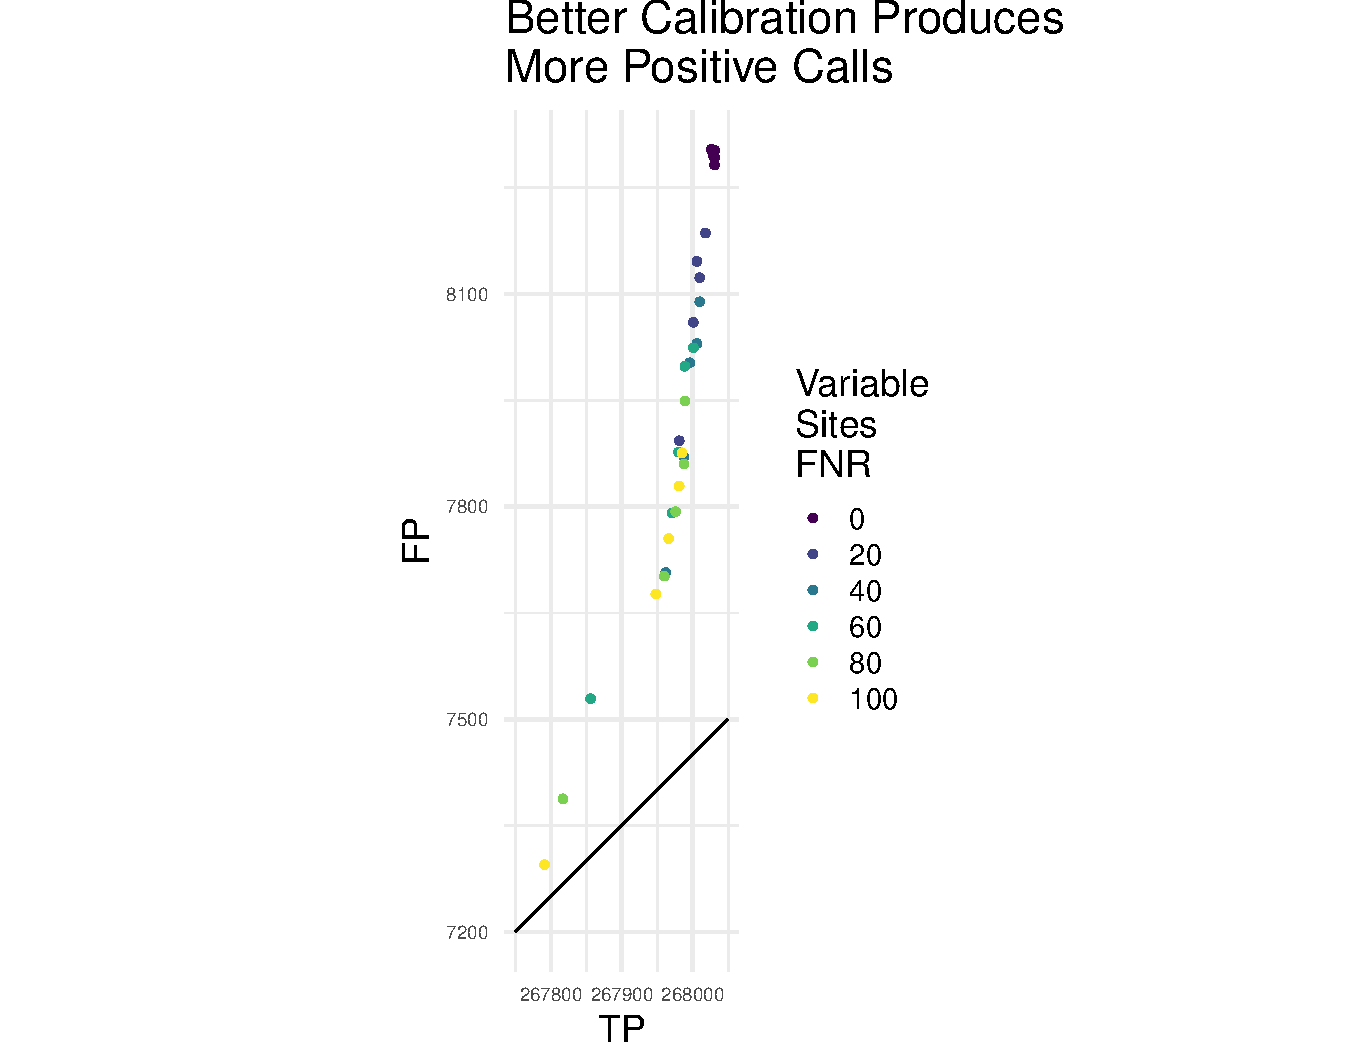
\includegraphics[width = .8\textwidth]{tp_fp_plot.pdf}
\titlecaption{More Accurate Known Sites Increases Number of Unfiltered Positive Calls}{The output number of positive calls for each dataset. The false negative rate of the set of variable sites used to calibrate the reads used to produce each callset is shown. As the false negative rate decreases, the number of both true positive and false positive calls increases. The raw, uncalibrated data exhibits the highest number of positive calls.}
\label{fig:vc_fptp}
\end{figure}

\begin{figure}
\centering
\includetwo{fp_heatmap.pdf}{tp_heatmap.pdf}
\titlecaption{Both False Negative and False Positive Rate Contribute to Increased Number of Unfiltered Positive Calls}{The output number of false positive calls for each dataset. The false negative and false positive rate of the set of variable sites used to calibrate the input reads or the name of the dataset for non-simulated datasets is shown on the X and Y axis. The color of each cell represents the number of unfiltered false positive (left) or true positive (right) SNP calls. As the false negative and positive rates of the database of variable sites decrease, the base quality scores become more calibrated, and more calibrated data produces more false positive and true positive calls. However, the raw data produces the most true positives and the most false positives.}
\label{fig:vc_p}
\end{figure}

To determine the impact of these variants on the overall quality of the callsets, I constructed heatmaps of the sensitivity and precision of each dataset (Figure \ref{fig:vc_sens_prech}). As the data become more well-calibrated, the sensitivity of the caller increases; however, the precision of the caller also decreases. This is also seen in the raw calibration: it has the highest sensitivity and lowest specificity of all the datasets. This means that the caller is able to detect more true variants, but a higher proportion of the calls it makes are false positives. To visualize the trade-off between sensitivity and precision, I plotted the precision against the sensitivity of each dataset, shown in Figure \ref{fig:vc_sens_prec}. To summarize the overall effect on accuracy, I show how the F-statistic changes across each dataset in Figure \ref{fig:vc_f_heatmap}. The callset made from the raw, uncalibrated data have the lowest F-statistic.

\begin{figure}
\centering
\includetwo{sensitivity.pdf}{precision.pdf}
\titlecaption{Better Calibration Increases Sensitivity and Reduces Precision}{The sensitivity (left) and precision (right) of the variant caller on each dataset with no filtering. As the base quality score calibration of the input reads increases, the sensitivity of the caller increases and the precision decreases. The data with raw quality scores has the highest sensitivity and lowest precision.}
\label{fig:vc_sens_prech}
\end{figure}

\begin{figure}
\centering
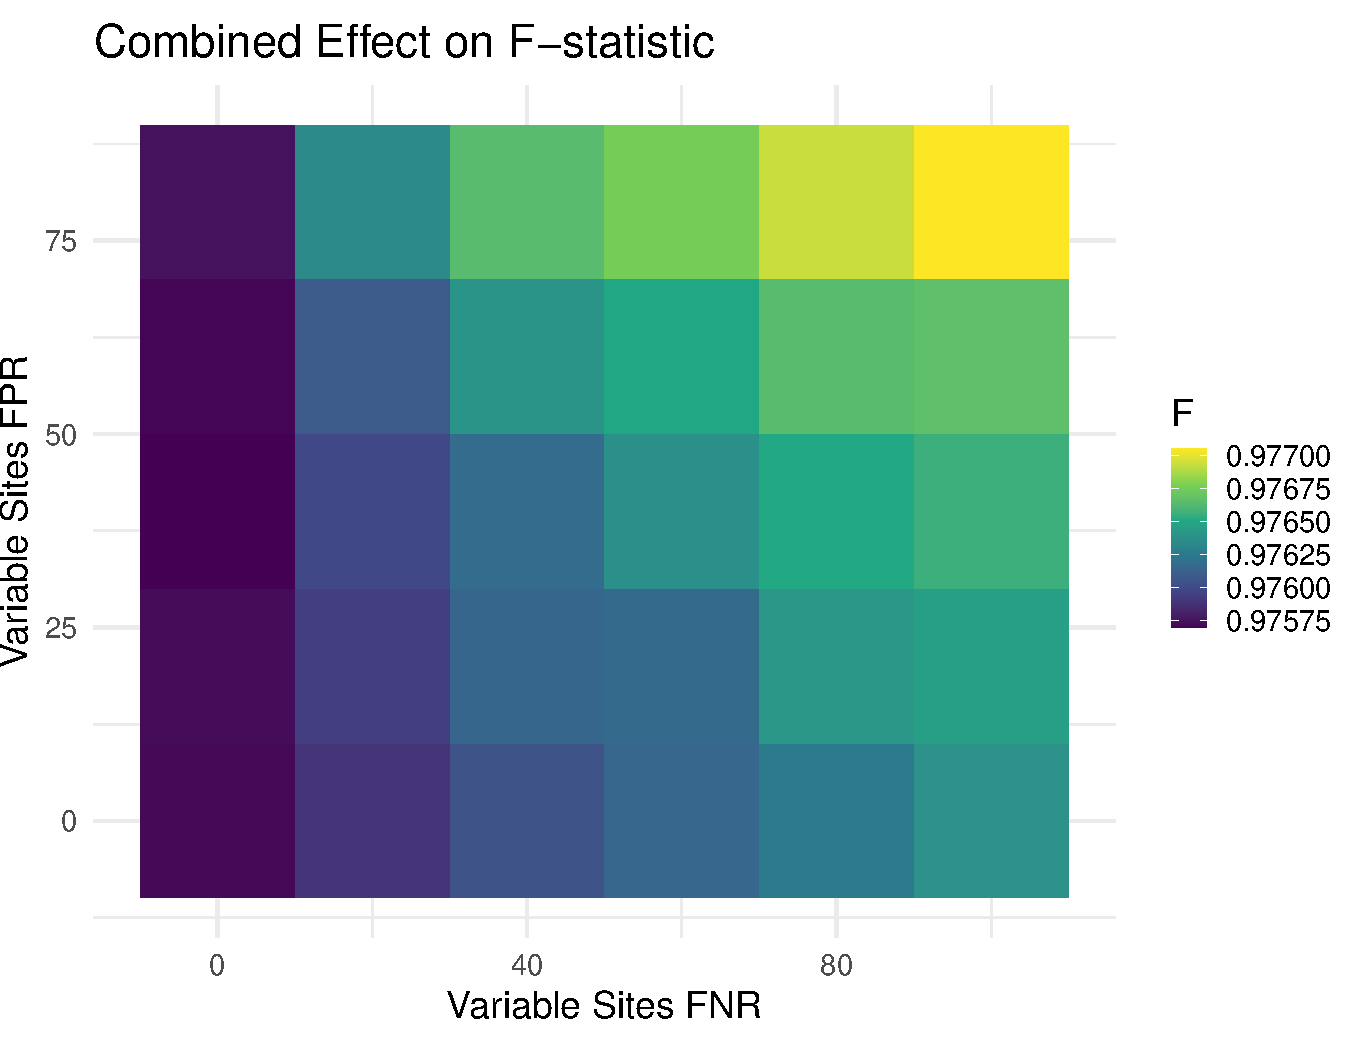
\includegraphics[width = .8\textwidth]{f_heatmap.pdf}
\titlecaption{F-statistic of Unfiltered Calls}{The F-statistic of the unfiltered calls of each dataset. As the base quality score calibration of the input reads increases, the F-statistic of the caller decreases. This is driven by the fact that the increase in sensitivity of the caller is much smaller than the decrease in precision. The raw, uncalibrated quality scores have the lowest F-statistic.}
\label{fig:vc_f_heatmap}
\end{figure}

Since the base quality score of the reads used to support each genotype call evidently play a role in whether to emit a variant, I wanted to see how the differences in calibration affected the annotations output by the caller. To that end, I plotted a receiver operating characteristic (ROC) curve showing how the false positive and true positive rates for variants ordered according to their QUAL and GQ annotations (Figure \ref{fig:vc_rocs}). These are both statistics that summarize the quality of the emitted site in a single, increasing score, and so are well-suited for ROC analysis. According to the VCF standard, the QUAL score is a phred-scaled probability that the ALT allele(s) present in the call are not actually present, $P($ALT is wrong$)$. The GQ score is the phred-scaled conditional probability the genotype call is incorrect given the site is variable, $P($genotype is wrong $|$ site is variant$)$.

\begin{figure}
\centering
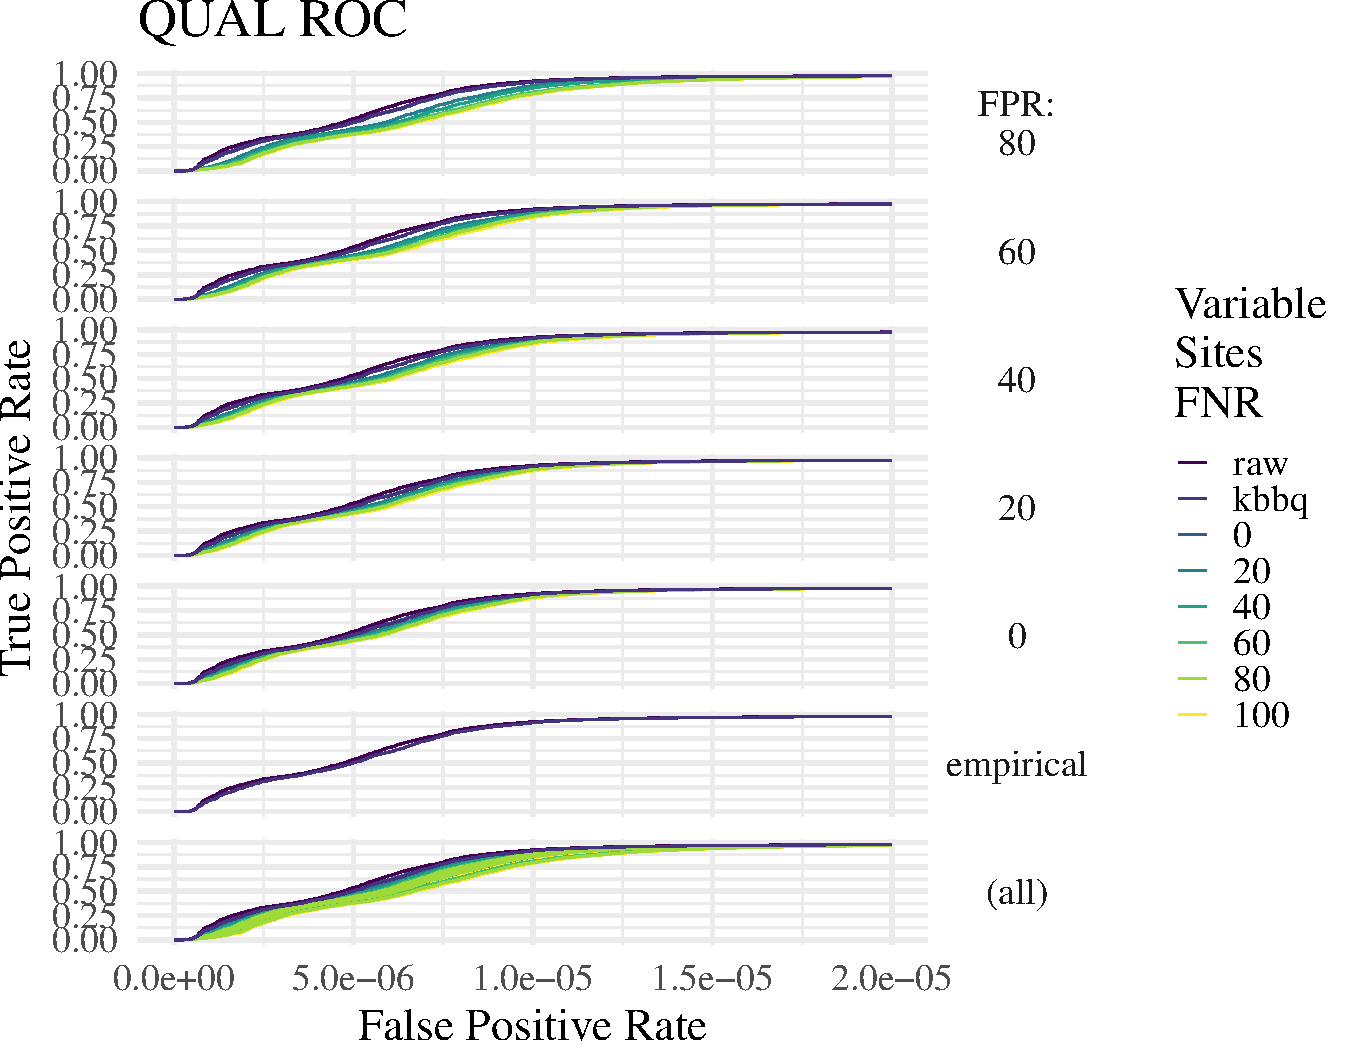
\includegraphics[width = .6\textwidth]{qualroc.pdf} \\
\vskip 1em
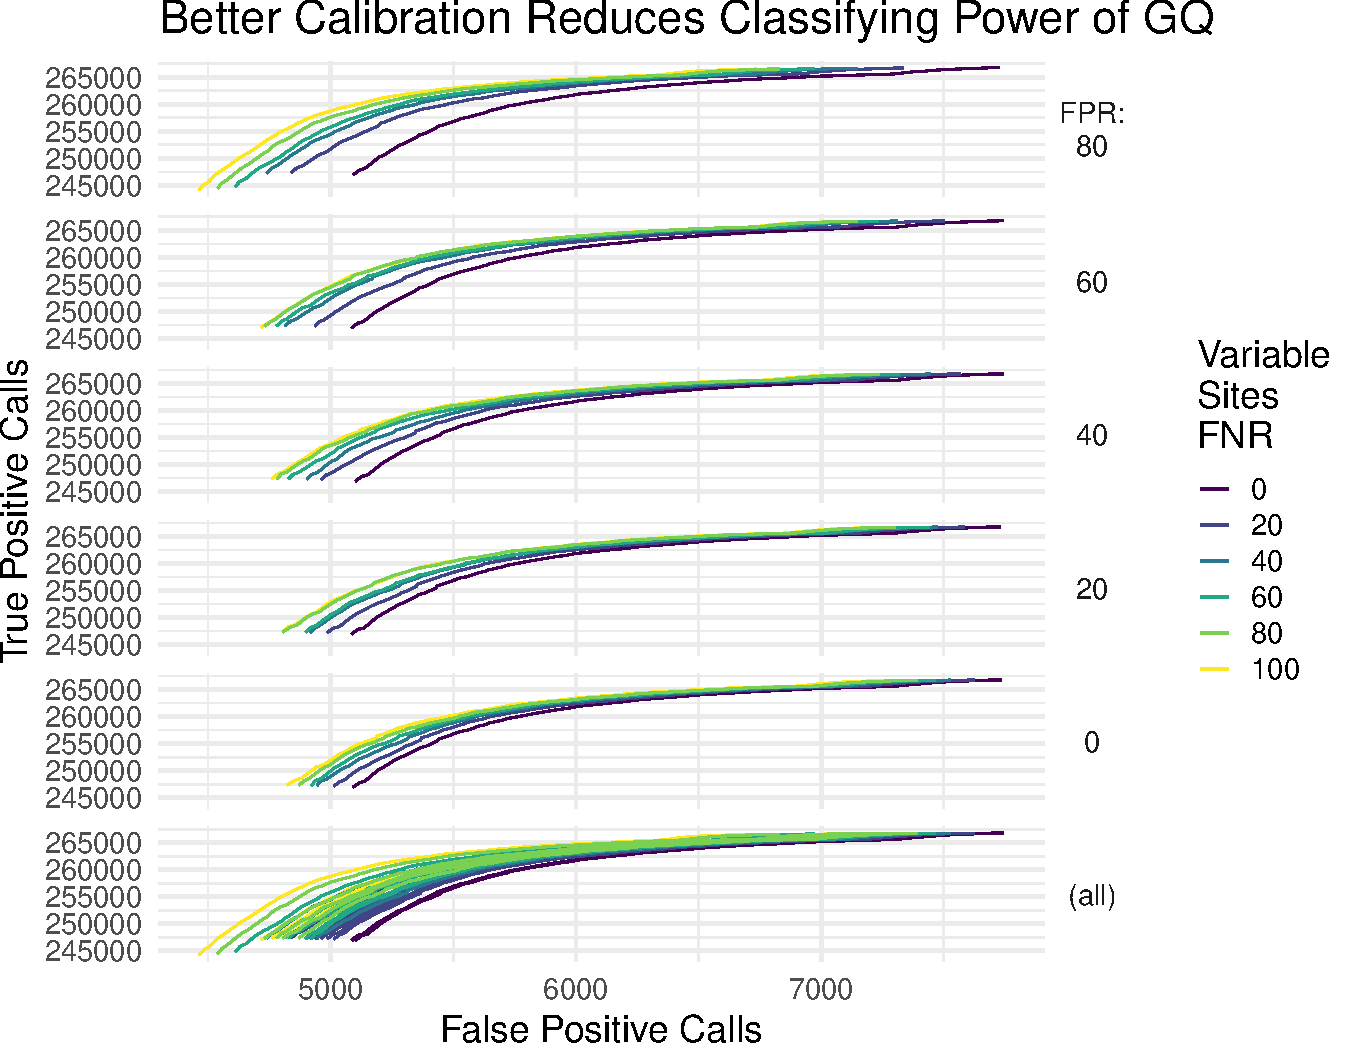
\includegraphics[width = .6\textwidth]{gqroc.pdf}
\titlecaption{Unfiltered ROC Curves}{The ROC curves for the QUAL (top) and GQ (bottom) score of an output call for the unfiltered calls of each dataset. The color of each line represents the false negative rate of the set of variant sites used as input to recalibrate the reads used to call variants. Each point in the line represents the number of false positive and false negative calls that have a score above the QUAL or GQ threshold for that point. As this threshold decreases, the number of false positives and true positives increases, though at different rates. These plots show that as the false positive rate increases, the number of true positive calls increases at a faster rate for the well-calibrated data than in other datasets for the QUAL classifier, but at a slower rate for the GQ classifier. The values for the two empirical datasets (raw and KBBQ), are shown on each plot. The other lines on each plot show values from calls made with reads that were recalibrated with variable site sets with the shown false positive rate.}
\label{fig:vc_rocs}
\end{figure}

As the ROC plots show that each dataset would respond to filtering differently, I examined how the calls would improve or not after filtration. I used a small QUAL filter filtering out variants with the lower 1\% of QUAL scores. This percentage coincides with the smallest QUAL value of the QUAL values that maximize the F-statistic of every dataset. These values are shown in Figure \ref{fig:vc_f_heatmap}. Depth filters are very common after variant calling, so I also used a depth filter to filter out calls that had unusually high or low depth.

% > rangedif <- function(x){range(x)[2] - range(x)[1]}
% > rangedif(df$TPc)
% [1] 313
% > rangedif(fltdf$TPc)
% [1] 3631
% > rangedif(df$FP)
% [1] 1858
% > rangedif(fltdf$FP)
% [1] 678

This resulted in a similar pattern of positive calls as the unfiltered data, seen in Figure \ref{fig:vc_flt_p}; better calibrated data had more false positive and true positive calls, and the raw dataset yielded the most positive calls. However, the difference between the number of true positive variants called from best-calibrated data and worst-calibrated was much larger after filtration. Before filtering, the largest difference between datasets was 313 true positive calls; this difference grows to 3631 after filtering. The opposite is observed for the false positive calls: before filtering, the largest difference in the number of false positive calls was 1858, but after filtering this difference decreases to 678. 
% Additionally, the difference between the number of true positives in the best-calibrated data and the next-best calibration at each step was smaller. So filtering caused even imperfectly-calibrated data to behave more like well-calibrated data, even though the extremes were further apart.                  %<- this is kinda weak
Ultimately, this alters the sensitivity and precision of each dataset such that the range of the sensitivity is increased and the range of the precision is decreased (see Figure \ref{fig:vc_flt_p}). This is sufficient to make the best-calibrated data also have the best F-statistic of all the simulated datasets, shown in Figure \ref{fig:vc_flt_f}. The calls made from the raw quality scores still has the best F-statistic overall.

\begin{figure}
\centering
\includetwo{flt_fp_heatmap.pdf}{flt_tp_heatmap.pdf}
\titlecaption{Filtered Positive Calls}{The output number of false positive and true positive calls for each dataset. The false negative and false positive rate of the set of variable sites used to calibrate the input reads is shown on the x and y axis. The color of each cell represents the number of false or true positive SNPs after filtering. As base quality scores become more calibrated, the number of positive calls increases. Note the range of positive calls has increased in comparison to each unfiltered dataset. Before filtering, the difference in the number of true positives between datasets was at most 240; after filtering it rises to 2044.}
\label{fig:vc_flt_p}
\end{figure}

% > rangedif(df$precision)
% [1] 0.003542063
% > rangedif(fltdf$precision)
% [1] 0.002312442
% > rangedif(df$recall)
% [1] 0.0008826549
% > rangedif(fltdf$recall)
% [1] 0.00748611

\begin{figure}
\centering
\includetwo{flt_sensitivity.pdf}{flt_precision.pdf}
\titlecaption{Filtered Call Sensitivity and Precision}{The sensitivity (left) and precision (right) of the variant caller on each dataset after filtering. As the base quality score calibration increases, the sensitivity of the caller increases and the precision decreases, as seen in the unfiltered data. However, the difference between the largest and smallest precision is slightly smaller than in the unfiltered data, and the difference between the largest and smallest recall is much larger.}
\label{fig:vc_flt_sp}
\end{figure}

\begin{figure}
\centering
\includetwo{sens_precision.pdf}{flt_sens_precision.pdf}
\titlecaption{Sensitivity and Precision Before and After Filtering}{The sensitivity and precision of the variant caller on each dataset with no filtering on the left, and after filters are applied on the right. In the unfiltered calls, as the base quality score calibration of the input reads decrease, the sensitivity of the caller decreases but its precision increases. Once the calls are filtered, the same pattern is observed. However, after filtering the range of precision between datasets is much smaller than before filtering. Conversely, the range of sensitivity increases.}
\label{fig:vc_sens_prec}
\end{figure}

\begin{figure}
\centering
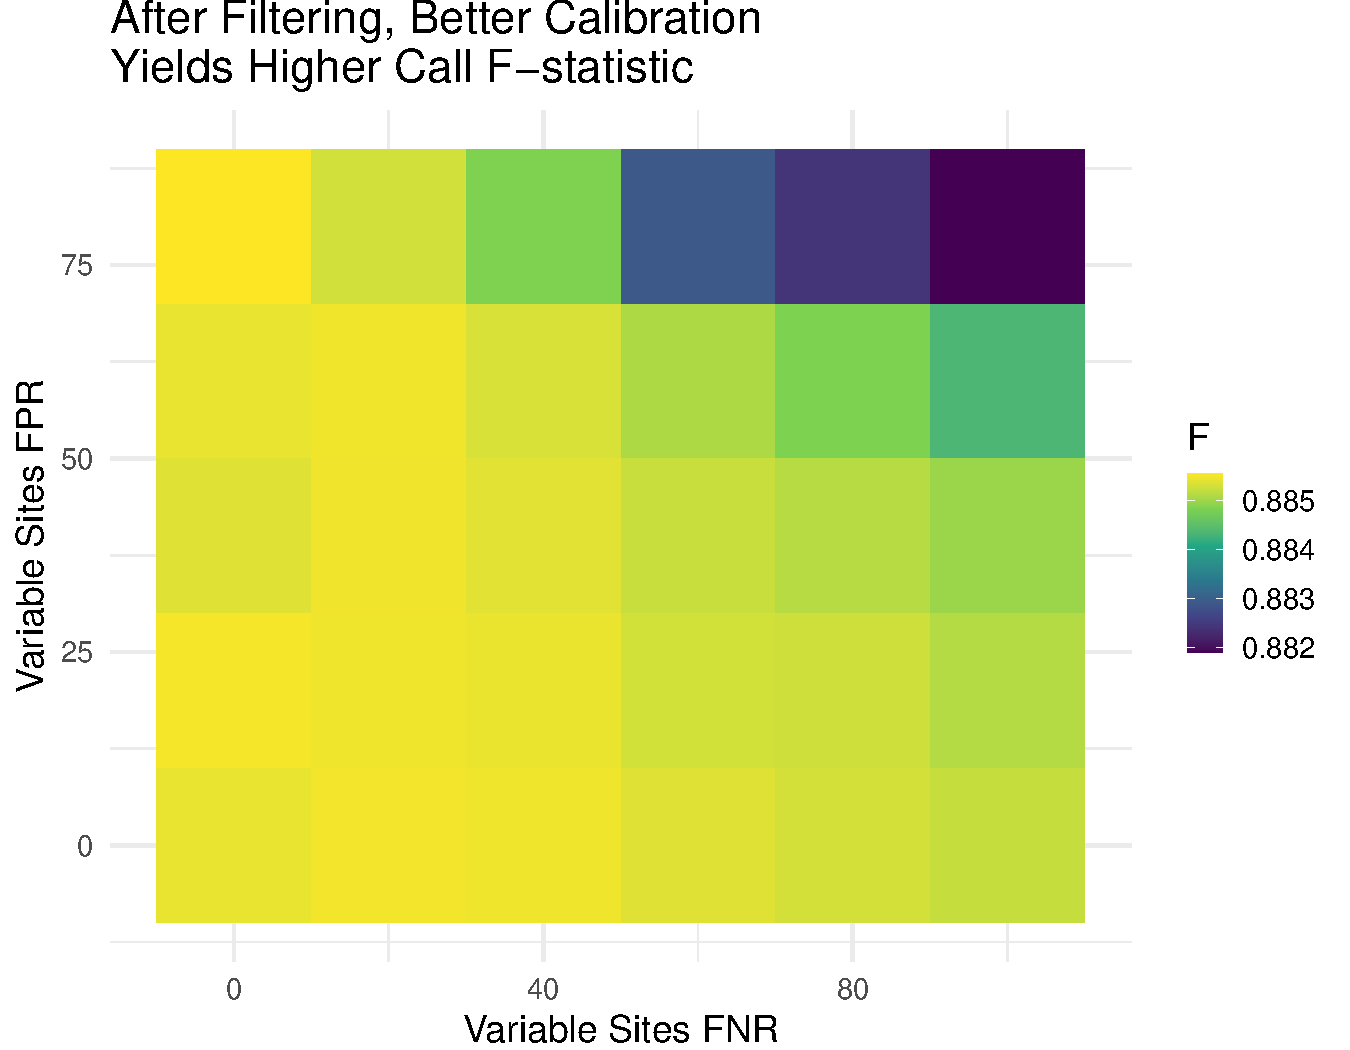
\includegraphics[width=.7\linewidth]{flt_f_heatmap.pdf}
\titlecaption{Filtered F-statistic}{The F-statistic of each dataset. As the calibration of the data improves, so does the F-statistic. This is in contrast to the unfiltered data, in which the worst-calibrated data has the best F-statistic. This difference is driven by an increase in relative precision of the best-calibrated data and a decrease in relative sensitivity of the poorly-calibrated data.}
\label{fig:vc_flt_f}
\end{figure}

%Simulated Reads results
Each of the three tested recalibration methods had only a small effect on the precision and sensitivity of HaplotypeCaller (see Figure \ref{fig:sim_sens_precision} and Table \ref{table:sim_summary}). The Initial-calls calibration did not change the precision compared to the raw quality scores, but did slightly decrease the sensitivity of the caller. GATK calibration using the true known variable sites yielded an increase in precision and sensitivity while the reference-free method KBBQ yielded an increase in precision but a slight decrease in sensitivity. Overall, this lead to an increase in the F-statistic after GATK recalibration with the true known sites and a decrease in the F-statistic after GATK recalibration with initial calls as the known sites, with no change in F-statistic after KBBQ recalibration. The ROC curve on the QUAL field of the called variants does not clearly show one calibration method as better than the others, and each one has the best trade-off between false positive and true positive rate at different points along the ROC curve except the Initial-calls calibration, which is closer to the bottom right of the plot at all times. There was no discernable difference between datasets when the GQ score was used to create the ROC curve, so it is not shown.

\begin{figure}
\centering
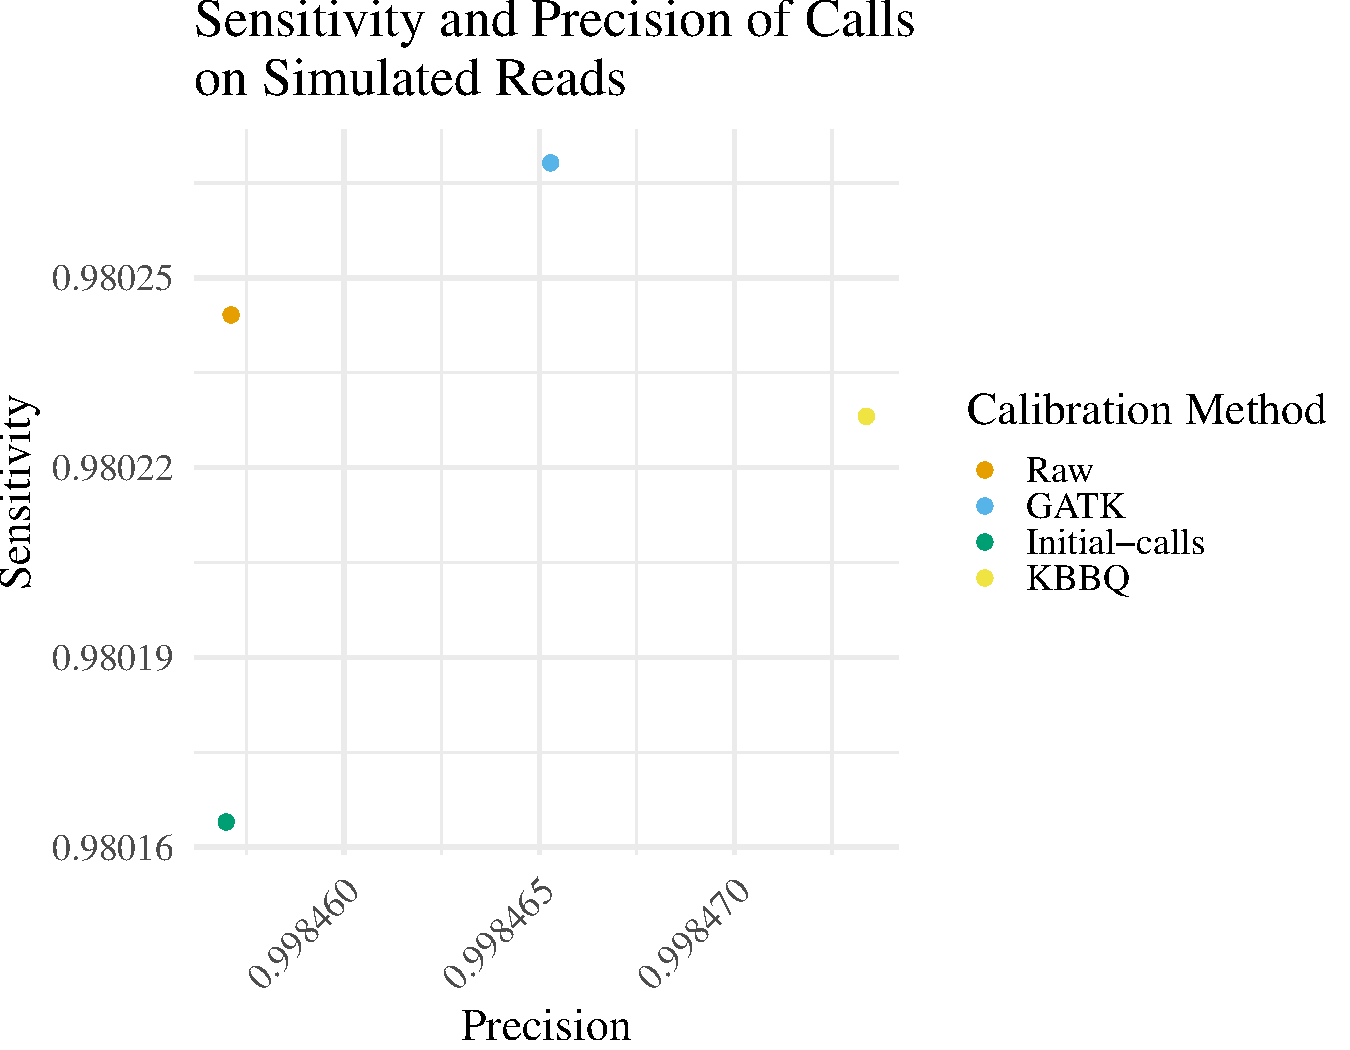
\includegraphics[width=.7\linewidth]{sims_sens_precision.pdf}
\titlecaption{Sensitivity and Precision of Calls on Simulated Reads}{The sensitivity and precision of calls made using the raw data and after recalibration with 3 methods. See Table \ref{table:sim_summary} for values plotted.}
\label{fig:sim_sens_precision}
\end{figure}

\begin{figure}
\centering
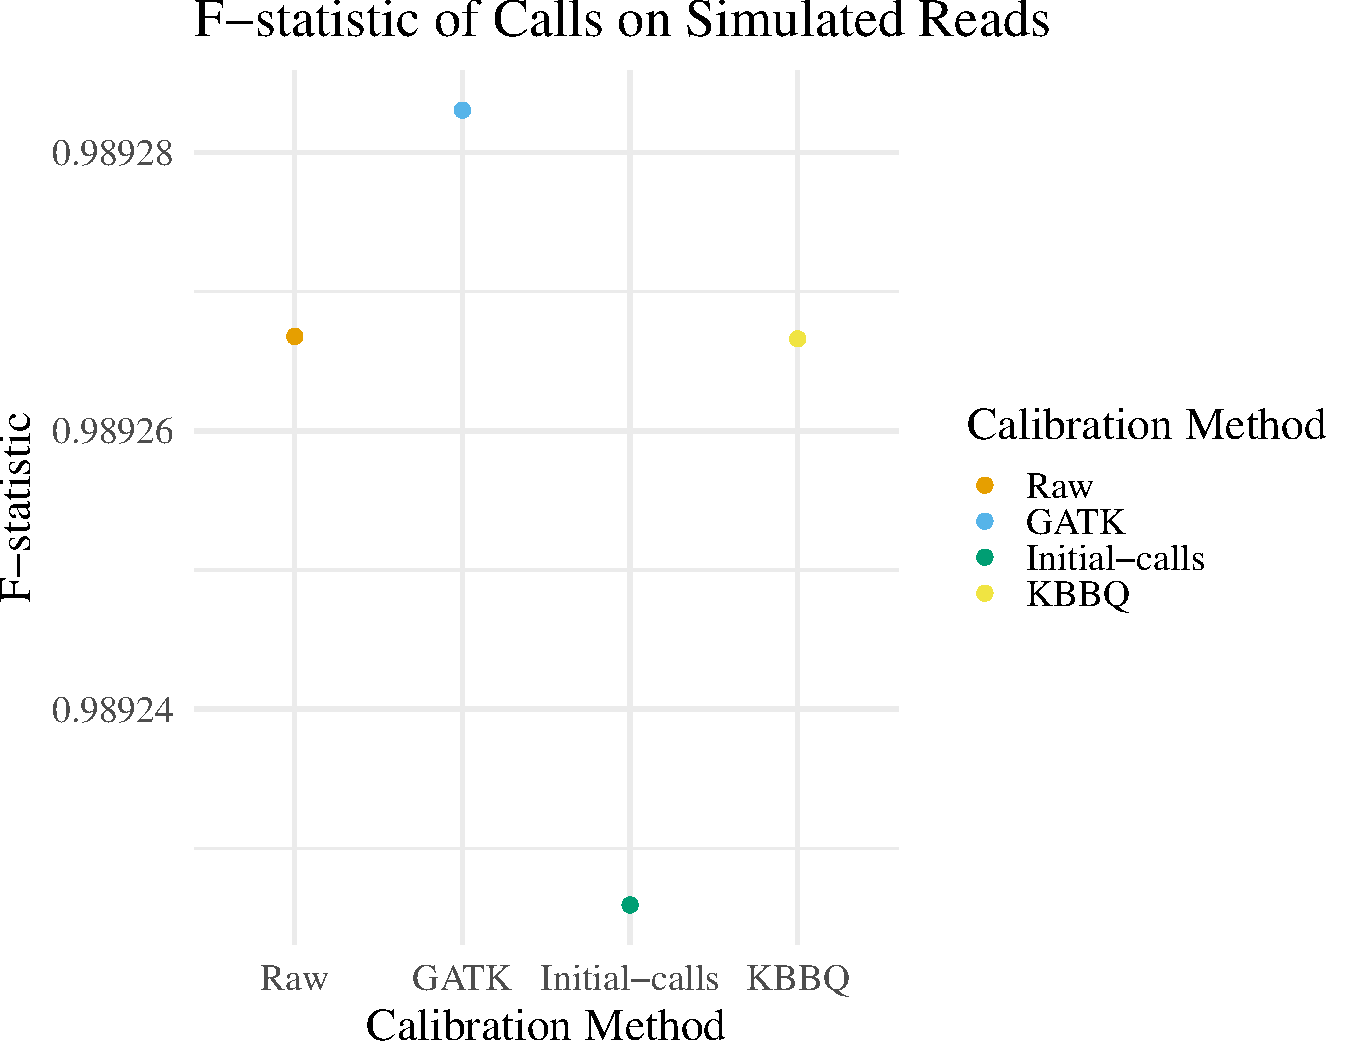
\includegraphics[width=.7\linewidth]{sims_fstat.pdf}
\titlecaption{F-statistic of Calls on Simulated Reads}{The F-statistic of calls made using the raw data and after recalibration with 3 methods. See Table \ref{table:sim_summary} for values plotted.}
\label{fig:sim_sens_precision}
\end{figure}

\begin{figure}
\centering
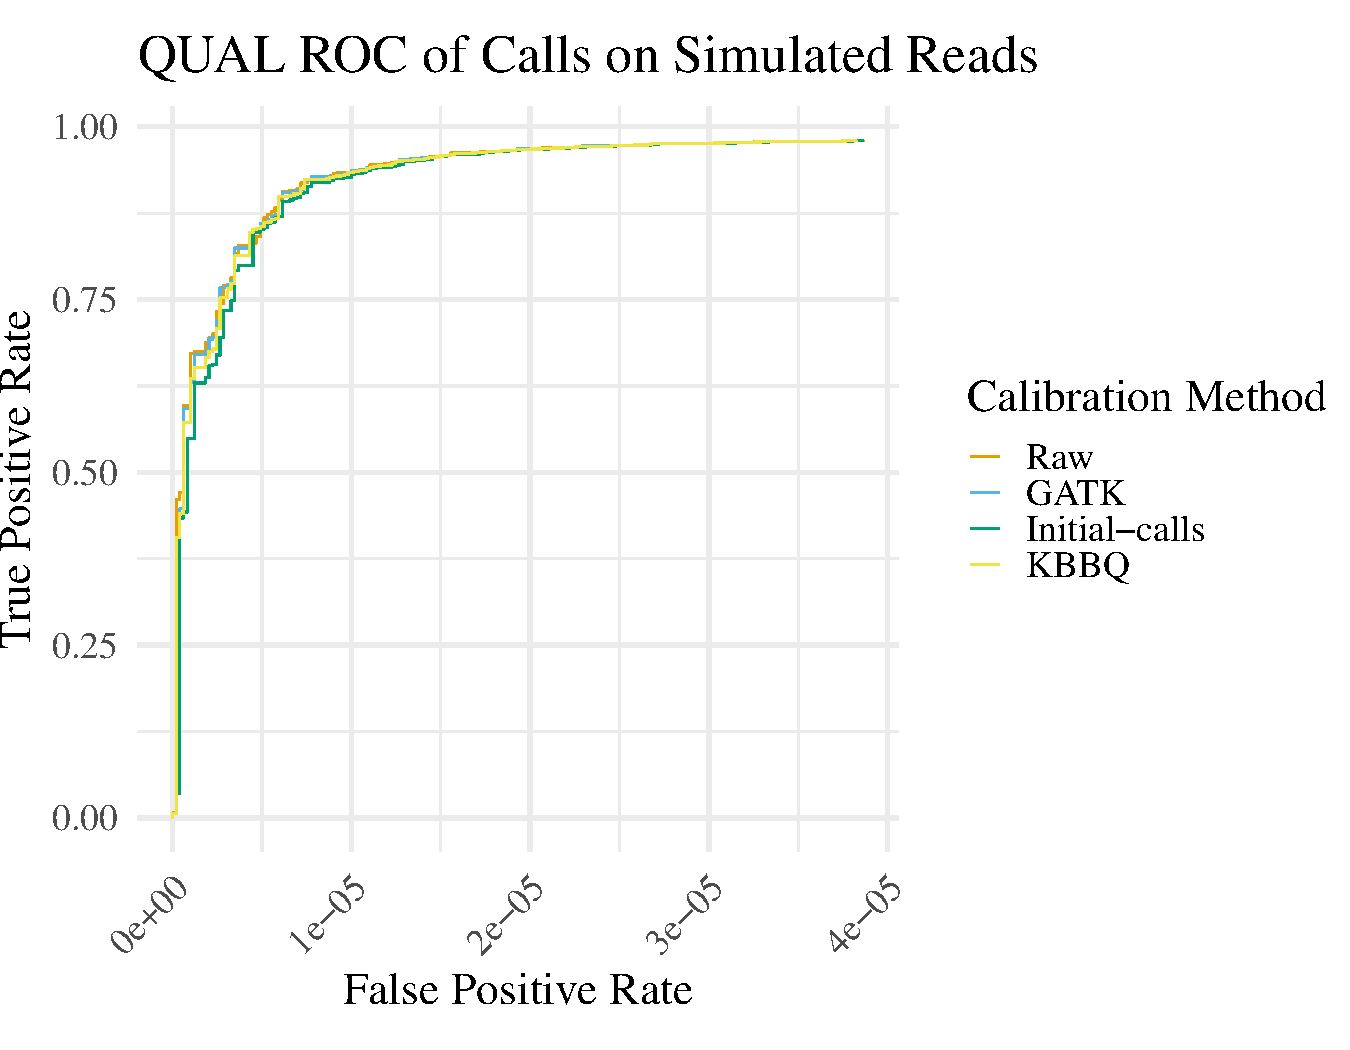
\includegraphics[width=.7\linewidth]{sims_qualroc.pdf}
\titlecaption{ROC of Calls on Simulated Reads}{ROC curve on the QUAL score of the variants called by HaplotypeCaller on the uncalibrated simulated reads and after recalibration with 3 methods.}
\label{fig:sim_qualroc}
\end{figure}


\begin{table}
\centering
\begin{tabular}{r l l l l l}
\toprule
Calibration Method & TP & FP & Sensitivity & Precision & F-statistic \\
\midrule
Raw & 122308 & 189 & 0.98024 & 0.99846 & 0.98927\\ 
GATK & 122311 & 188 & 0.98027 & 0.99847 & 0.98928\\ 
Initial-calls & 122298 & 189 & 0.98016 & 0.99846 & 0.98923\\ 
KBBQ & 122306 & 187 & 0.98023 & 0.99847 & 0.98927\\ 
\bottomrule
\end{tabular}
\titlecaption{Variant Caller Performance on Simulated Data}{A summary of the performance of HaplotypeCaller on simulated data calibrated different ways. TP is the number of true positive calls and FP the number of false positive calls. Raw is the quality scores assigned by the simulator, GATK is recalibration using the known heterozygous sites, Initial-calls is recalibration after calling an initial set of variants, and KBBQ is recalibration with the reference-free recalibrator KBBQ. See Figure \ref{fig:sim_sens_precision} for a visual comparison.}
\label{table:sim_summary}
\end{table}



\subsection{Variants Detected in \textit{E. melliodora}}

In order to determine the effect of reference-free recalibration on variant calls, I recalibrated the reads with the reference-free base quality score recalibrator KBBQ (see Chapter \ref{ch:kbbq} for more information on KBBQ). I then called variants and filtered the same way they were called and filtered in \cite{orr_phylogenomic_2020}. The number of variants called at each step in the filtering process is shown in Table \ref{tbl:num_variants}. The number of variants called at each step using uncalibrated reads is shown in Table \ref{tbl:num_raw_variants}. After filtering, 106 variants were detected; 34 of these were also detected in the confident set of variants previously identified. This previous set had a total of 90 variants. Filtering reduced the average number of false positive variants estimated to 35.54. Note that the number of detected sites listed in Table \ref{tbl:num_variants} are not all indicative of mutation, as the number includes heterozygous sites until the last filtering step.

\begin{table}
\begin{tabularx}{\textwidth}{>{\hsize=1.5\hsize\linewidth=\hsize}X >{\hsize=.7\hsize\linewidth=\hsize}X >{\hsize=.9\hsize\linewidth=\hsize}X >{\hsize=.9\hsize\linewidth=\hsize}X}
\toprule
\textbf{Description} & \textbf{Num.\newline{}Variants} & \textbf{Estimated\newline{}False Positives} & \textbf{True\newline{}Positives}\\
% & \textbf{Variants} & \textbf{False Positives} & \textbf{Positives} \\
\midrule
Appears in first 11 scaffolds & 9838408 & 911.46 & 88\\
Total depth <= 500 & 9190223 & 800.83 & 87\\
ExcessHet <= 40 & 4932628 & 144.95 & 86\\
Not within 50bp of an indel & 3175128 & 85.05 & 69\\
Biallelic SNPs & 1913594 & 68.88 & 67\\
Outside repeat regions & 857810 & 35.54 & 46\\
All 3 replicates match & 63793 & - & 35\\
Only variable sites & 106 & - & 34\\
\bottomrule
\end{tabularx}
\titlecaption{Number of Detected Variants After KBBQ Recalibration}{The number of variants detected at each step in the filtering pipeline. Each row includes a description of each filter and the number of variants remaining after the filter has been applied. It also includes the number of false positives estimated by simulating 100 random, maximally distant trees, using those trees to filter the result at each step, and averaging the number of variants that survive filtering. Since step 7 includes filtering based on replicate agreement, this method cannot detect false positives for step 7 or 8; in the worst case, they are identical to the number of estimated false positives in step 6. True positives were estimated using the number of variants ultimately detected in the confident set described in \cite{orr_phylogenomic_2020}. This set contains a total of 90 variants.}
\label{tbl:num_variants}
\end{table}

\begin{table}
\begin{tabularx}{\textwidth}{>{\hsize=1.5\hsize\linewidth=\hsize}X >{\hsize=.7\hsize\linewidth=\hsize}X >{\hsize=.9\hsize\linewidth=\hsize}X >{\hsize=.9\hsize\linewidth=\hsize}X}
\toprule
\textbf{Description} & \textbf{Num.\newline{}Variants} & \textbf{Estimated\newline{}False Positives} & \textbf{True\newline{}Positives}\\
% & \textbf{Variants} & \textbf{False Positives} & \textbf{Positives} \\
\midrule
Appears in first 11 scaffolds & 9823414 & 915.96 & 88\\
Total depth <= 500 & 9177547 & 804.91 & 87\\
ExcessHet <= 40 & 4924104 & 144.6 & 86\\
Not within 50bp of an indel & 3169769 & 85.68 & 69\\
Biallelic SNPs & 1911802 & 68.76 & 67\\
Outside repeat regions & 858383 & 36.54 & 46\\
All 3 replicates match & 63687 & - & 35\\
Only variable sites & 88 & - & 34\\
\bottomrule
\end{tabularx}
\titlecaption{Number of Detected Variants Using Uncalibrated Reads}{The number of variants detected at each step in the filtering pipeline using uncalibrated reads. See Table \ref{tbl:num_variants}.}
\label{tbl:num_raw_variants}
\end{table}

\section{Discussion}
\label{sec:kbbq_discussion}

These results show that GATK BaseRecalibrator is particularly vulnerable to false negatives (Figure \ref{figure:fnr}) in the database of variable sites, but is robust to false positives if the false negative rate is near 0 (Figure \ref{figure:fpr}). At the same time, when the false negative rate is not near 0, false positives will start to impact the calibration quality (Figure \ref{figure:fnrfpr}). Thus, when this database is unavailable and construction is required, it may be better to be liberal in deciding which sites may be variable to reduce the false negative rate as much as possible. This is in contrast to the GATK recommendation to use only the most confident sites when a database is unavailable.

The only rate that shows significant deviation from a 0\% false positive rate in the false-positive-only data is the 100\% false positive rate. Though a 100\% false positive rate with a 0\% false negative rate implies every site should be considered variable and ignored, the model curiously still has a source of errors it uses to recalibrate. Upon further investigation, this effect is driven by reads with alignments that begin with an insertion, as these inserted bases are not ignored by BaseRecalibrator when the first position of the site that should be ignored is equal to the first aligned position in the read. Thus, this line is a technical artifact. So long as there are enough bases available to analyze, the false positive rate doesn't significantly affect the performace of BaseRecalibrator at a false negative rate of 0. The calibrations of other datasets with a false positive rate of 100\% would also be affected by this artifact; however, in a real dataset it's unlikely to ever achieve a false positive rate of 100\%, so this artifact is unlikely to significantly affect real data.

%new para
Ultimately, if the false negative and false positive rates of the database of variable sites is high, GATK's procedure for BQSR \textit{can} cause miscalibration of the data worse than using raw quality scores, though this can only happen with very large error rates. In this dataset, the raw data has a RMSE of about 4, which is similar to a simulated dataset with a false negative rate between 40-60\% and a false positive rate between 60-80\%. In a real situation it's unlikely that error rates like this will occur, so BQSR will not severely destroy the input data. However, at even modest false negative and false positive error rates BQSR can cause undesirable miscalibration that could feasibly impact variants called from the data. Interestingly, at all error rates the calibration of quality scores below 25 is almost always correct or 1-off the true value. It seems that errors in the database of variable sites have a larger effect on higher quality predictions than lower ones.

Interestingly, overconfidence is not displayed in the reads recalibrated using the artificially constructed database of variable sites. This is likely because of how these variant sets were constructed; non-variable sites were selected independently and at random to be added to the set of purported variable sites. Thus a site containing an error and a site not containing an error are selected proportionally. In contrast, on a real dataset a variant calling algorithm would not make false positive errors independently; it is much more likely to classify a site as variable that has a sequencing error than to classify a site as variable that has no errors. That is: in this simulation, $P(\operatorname{classified\:positive} | \operatorname{actual\:negative})$ is independent of $P(\operatorname{sequencing\:error})$, but on an empirical dataset $P(\operatorname{classified\:positive} | \operatorname{actual\:negative})$ is likely not. Thus in reality false positives probably cause overconfidence in a similar manner that false negatives cause underconfidence.

Overall, these results show that as the quality of the calibration increases, the quality of the variant calls also slightly increases. The difference is very small, but better calibration produces more positive calls, with more true positive calls than any other recalibrated dataset. And though I only filtered the data with two fairly lenient filters, the best calibrations still produced the most true positive calls of any dataset. The exception to this is the calls made from data with the raw quality scores, which are not as well-calibrated (see Chapter \ref{ch:kbbq}) but produce more positive calls.

Interestingly, filtering seemed to amplify the difference between well-calibrated and poorly-calibrated data, increasing the disparity in the number of true positive variants detected. At the same time, filtering reduced the disparity in the number of false positive variants identified.

%Talk about how filtering becomes very important for leveraging the power of calibration
This observation makes filtering very important for variant calling. Variant callers generally prefer to include a putative variant rather than exclude it and miss a truly variant site. Thus, they prefer sensitivity over precision. The consequences of this preference can be seen in Figure \ref{fig:vc_sens_prec}, where filtering reduced the sensitivity of every set of calls but greatly improved precision and decreased the precision disparity between datasets. Filtering raw calls is paramount to getting a variant set with acceptable levels of sensitivity and precision. Ultimately, the impact of base quality score recalibration is not as large as the filters one chooses to use. In this case, better calibration results in an increased precision of .007 before filtering; filtering itself increased precision by about .014, while reducing sensitivity by approximately .18. So the effect of calibration on sensitivity and precision is small in comparison to the effect of filtering. At the same time, important variants that matter for the purposes of the study being conducted could be missed, so this difference in calibration could be relevant.

Unfortunately, this means that filtering plays a big role in the success of a variant calling pipeline. While there is no definitive best way to filter variants in all cases, Figure \ref{fig:vc_rocs} shows that differences in quality score calibration can affect the annotations attached to each call and make the same filters more or less effective, depending on the threshold used. While this is interesting, it doesn't necessarily change how filtering should be done or suggest an optimal filtering strategy.

One limitation of this study is that is uses only a single dataset and only a sparse range of false positives and false negatives in the database of variable sites. Especially since the effect of calibration on the output variant calls is small, a different dataset may yield different results. As seen in Chapter \ref{ch:kbbq}, the calibration of the raw reads in this dataset is not particularly bad, though it is worse than all other datasets. Replication with other datasets and other variant callers is necessary to further elucidate the role of base quality score calibration on variant caller performance.

Furthermore, this data is from a human-derived cell line, and protocols for DNA extraction and sequencing are fairly well-established. Additionally, the original base calling algorithm is likely tuned to work well with human-like data. All together, this means that while the effect of recalibration was not particularly pronounced in this dataset, base quality score recalibration may have a higher impact on data that is messier, contains more errors induced in sample preparation, or results from failed sequencing runs. In light of this, it seems that using the default-assigned base quality scores will offer superior performance unless one has a reason to suspect the data is of poor quality.

% Simulated Data
% Each of the three tested recalibration methods had only a small effect on the precision and sensitivity of HaplotypeCaller (see Figure \ref{fig:sim_sens_precision} and Table \ref{table:sim_summary}). The Initial-calls calibration did not change the precision compared to the raw quality scores, but did slightly decrease the sensitivity of the caller. GATK calibration using the true known variable sites yielded an increase in precision and sensitivity while the reference-free method KBBQ yielded an increase in precision but a slight decrease in sensitivity. Overall, this lead to an increase in the F-statistic after GATK recalibration with the true known sites and a decrease in the F-statistic after GATK recalibration with initial calls as the known sites, with no change in F-statistic after KBBQ recalibration. The ROC curve on the QUAL field of the called variants does not clearly show one calibration method as better than the others, and each one has the best trade-off between false positive and true positive rate at different points along the ROC curve except the Initial-calls calibration, which is closer to the bottom right of the plot at all times. There was no discernable difference between datasets when the GQ score was used to create the ROC curve, so it is not shown.

The simulated reads similarly show that the effect of base quality score recalibration is fairly small. However, the simulator also assigned fairly well-calibrated scores to begin with, so there is not much room for improvement in those scores and many opportunities to make calibration worse. As shown in the previous chapter, using initial calls for recalibration does degrade the overall quality of the calibration. This is consistent with these results showing that HaplotypeCaller performs worse on reads recalibrated using GATK with a set of initial calls. However, when the set of known sites is the true set of variable sites in the data, GATK recalibration does slightly improve the precision and sensitivity of HaplotypeCaller. At the same time, reference-free recalibration with KBBQ increases precision but slightly decreases sensitivity.

Overall, these simulations show that GATK recalibration slightly increases HaplotypeCaller performance if the set of variable sites is complete and has no false positives, even if the starting data is fairly well-calibrated. However, if the set of variable sites is not complete, GATK recalibration will cause HaplotypeCaller performance to suffer slightly. Thus, if there is a risk that the set of variable sites is inaccurate, GATK recalibration should not be used. At the same time, raw quality scores will provide good performance as long as they are fairly well-calibrated to start. These simulations also show that even with well-calibrated input data, the reference-free recalibration method KBBQ doesn't significantly degrade the performance of HaplotypeCaller.

%



%Speculate about when BQSR might actually be useful!! More work is needeD!!!

% Surprisingly, the behavior of the raw dataset is most similar to that of KBBQ and the dataset calibrated with perfect information. At the same time, the patterns observed clearly indicate an effect of calibration on how HaplotypeCaller functions. This can be explained in a few ways; 1) GATK's own calibration method is flawed, and the raw data is truly the best calibrated data, so the trends are real. 2) this dataset is just weird 3) the calibration is actually correct and calibration affects HC in a roundabout way that doesn't directly translate into better calls. The trends are an artifact of that process.

\subsection{KBBQ Recalibration Improved \textit{E. melliodora} Calls}

While the simulated datasets revealed a complex interaction between the number of detected variants, sensitivity, precision, and filtering, it appears KBBQ recalibration improved the ability to successfully call variants in a non-model organism. In Chapter \ref{ch:kbbq}, I showed that using GATK's recommended approach of calling confident variants and using those as the set of variable sites to use in recalibration results in poor base quality score calibration. I also showed that using KBBQ improved calibration to be comparable to GATK recalibrations with perfect information. The calls on the simulated datasets shown here also imply that KBBQ recalibrated reads behave similarly to or better than reads recalibrated with GATK using perfect information.

Using the same calling and filtering parameters as those used in \cite{orr_phylogenomic_2020} yielded more variants at the end of filtering with 106 instead of 99. This is consistent with the results from the simulated datasets, where better-calibrated data yields more variant calls. It is also consistent with \cite{ni_improvement_2016}, who find that better calibration increases sensitivity. Indeed, this is the case even before other filters are applied, with 9,838,408 variants detected versus 9,679,544 detected in the prior study. This is also slightly more than the 9,823,414 detected using uncalibrated reads before filtering and 88 detected after.

Additionally, the number of variants after filtering that appear in the confident set identified in the previous study increased from 30 to 34. This is identical to the number detected using the raw reads. However, in contrast to the results from the simulated data, the number of estimated false positive calls decreased as well in the KBBQ recalibrated data, falling from 55.71 to 35.54 after filtering and from 1033.18 to 911.46 before filtering. The variants called using KBBQ recalibrated data have slightly fewer false positive calls than the variants called using the raw data, with the GATK method yielding the most false positives. This is consistent with \cite{ni_improvement_2016} and \cite{li_improving_2011} who find that better quality score calibration reduces the number of false positive calls. Thus, using KBBQ to recalibrate the reads before calling seems to have substantially increased both the sensitivity and the precision of the variant calling pipeline compared to GATK's BaseRecalibrator and using raw quality values.

After all filters were applied, the pipeline yielded 106 mutations with an estimated 36 false positives and 34 previously-estimated true positives. This leaves approximately 36 positive variants that were not in the set of previously identified variants. This is an approximately 2.8 times increase from that same estimate of 13 inferred with the same pipeline from \cite{orr_phylogenomic_2020}, except using KBBQ rather than BaseRecalibrator. It is a 2 times increase from the same estimate of 18 using the same pipeline but uncalibrated reads. While this is an estimate based on the false positive rate and so cannot be used to distinguish between previously unidentified true variants and false positives, it shows how the decrease in false positive rate and increase in number of calls using KBBQ recalibrated reads improves the overall ability of the variant calling pipeline to reveal true mutations.

\section{Conclusion}

The simulated data here shows that quality scores do have a small but important effect on the quality of the called variants. This manifests itself in not only the difference in the number of true positive calls and the number of false positive calls, but also in the QUAL and GQ annotations. The simulated data suggest the size of the effect is small, but on an empirical dataset the size of the effect was much larger; this could be due to differences in reference quality and species-specific biases in base calling. While effective recalibration will certainly benefit variant calling, the empirical data here show BaseRecalibrator can decrease the quality of the called variants if done improperly. If very high sensitivity is critical to the analysis being performed, care must be taken to ensure that base quality scores are properly calibrated.

\printbibliography[segment=\therefsegment]{}

\chapter{Conclusion}

While noisy sequencing data can be difficult to work with, with care it \textit{is} possible to generate high-quality calls. As both sequencing technology and software tools improve, the amount of useful information that can be extracted from sequencing experiments will continue to grow, and the costs of performing those experiments will continue to shrink. This will enable the generation of an unprecedented amount of data, particularly in organisms that have been historically neglected. This necessitates the continued development of methods that function even without \textit{a priori} information.

All together, the experiments included here show that while calling variants requires effort when reference genomes and other information is not available, it is not impossible. Most methods designed to work with reference-aligned data can work fairly well if a reference from a close relative can be adapted to the data, as shown in Chapter \ref{ch:phylogenomic}. Furthermore, Chapter \ref{ch:kbbq} shows that base quality scores can be successfully calibrated without any auxiliary information. And Chapter \ref{ch:evaluating} shows that this improvement in base quality score calibration can improve variant calling sensitivity and reduce the number of false positive calls.

In these investigations, I have highlighted and developed several methods for detecting mutations in non-model organisms. While the data used here is limited to Illumina short read sequencing, the approaches described are adaptable for even the next generation of sequencing platforms. The principles discussed and their application may prove even more useful on these platforms, as their primary drawback is high error rates. Even now, computational methods are able to overcome the error rates on these platforms and make them suitable for some applications, like assembly.

Now is an incredible time to be interested in sequencing and sequencing technology. Illumina sequencing and associated methods are relatively mature, but interesting new methods and models are still expanding the limits of the technology and achieving impressive results despite its flaws. On the horizon, long read sequencing is becoming ever more affordable, accurate, and fast, promising new avenues for investigating the natural world along with new challenges. But no matter what the future holds, one thing is clear: software and statistical methods for analyzing sequencing data will continue to be necessary to get the most out of sequencing technology and transform raw data into insights.



% As the process becomes cheaper and cheaper, the pace of data generation is expected to accelerate. Scientists will need a wide-range of computational tools available to them to succeed in their investigations. Thus, it behooves those of us who write such tools to be clear about their assumptions and limitations and to make our tools simple to install and use, while making them difficult to misuse and abuse. Interoperability and common standards will also be necessary to ensure the increasing amount of data collected turns into increasing knowledge and not wasted effort.

%-----------------------back matter
\newpage
{\singlespace
% Making the references a "part" rather than a chapter gets it indented at
% level -1 according to the chart: top of page 4 of the document at
% ftp://tug.ctan.org/pub/tex-archive/macros/latex/contrib/tocloft/tocloft.pdf
\addcontentsline{toc}{part}{REFERENCES}
% \bibliographystyle{asudis}
%\bibliography{dis}

\printbibliography{}
% \printbibheading[title=References]{}
% \bibbysection{}
}
\renewcommand{\chaptername}{APPENDIX}
\addtocontents{toc}{APPENDIX \par}
\appendix
\chapter{Permission to include previously published work}
\label{ch:permission}

TODO: list permission here.

\chapter{RAW DATA}

\include{vita}
\end{document}